\documentclass[twoside]{book}

% Packages required by doxygen
\usepackage{fixltx2e}
\usepackage{calc}
\usepackage{doxygen}
\usepackage[export]{adjustbox} % also loads graphicx
\usepackage{graphicx}
\usepackage[utf8]{inputenc}
\usepackage{makeidx}
\usepackage{multicol}
\usepackage{multirow}
\PassOptionsToPackage{warn}{textcomp}
\usepackage{textcomp}
\usepackage[nointegrals]{wasysym}
\usepackage[table]{xcolor}

% Font selection
\usepackage[T1]{fontenc}
\usepackage[scaled=.90]{helvet}
\usepackage{courier}
\usepackage{amssymb}
\usepackage{sectsty}
\renewcommand{\familydefault}{\sfdefault}
\allsectionsfont{%
  \fontseries{bc}\selectfont%
  \color{darkgray}%
}
\renewcommand{\DoxyLabelFont}{%
  \fontseries{bc}\selectfont%
  \color{darkgray}%
}
\newcommand{\+}{\discretionary{\mbox{\scriptsize$\hookleftarrow$}}{}{}}

% Page & text layout
\usepackage{geometry}
\geometry{%
  a4paper,%
  top=2.5cm,%
  bottom=2.5cm,%
  left=2.5cm,%
  right=2.5cm%
}
\tolerance=750
\hfuzz=15pt
\hbadness=750
\setlength{\emergencystretch}{15pt}
\setlength{\parindent}{0cm}
\setlength{\parskip}{0.2cm}
\makeatletter
\renewcommand{\paragraph}{%
  \@startsection{paragraph}{4}{0ex}{-1.0ex}{1.0ex}{%
    \normalfont\normalsize\bfseries\SS@parafont%
  }%
}
\renewcommand{\subparagraph}{%
  \@startsection{subparagraph}{5}{0ex}{-1.0ex}{1.0ex}{%
    \normalfont\normalsize\bfseries\SS@subparafont%
  }%
}
\makeatother

% Headers & footers
\usepackage{fancyhdr}
\pagestyle{fancyplain}
\fancyhead[LE]{\fancyplain{}{\bfseries\thepage}}
\fancyhead[CE]{\fancyplain{}{}}
\fancyhead[RE]{\fancyplain{}{\bfseries\leftmark}}
\fancyhead[LO]{\fancyplain{}{\bfseries\rightmark}}
\fancyhead[CO]{\fancyplain{}{}}
\fancyhead[RO]{\fancyplain{}{\bfseries\thepage}}
\fancyfoot[LE]{\fancyplain{}{}}
\fancyfoot[CE]{\fancyplain{}{}}
\fancyfoot[RE]{\fancyplain{}{\bfseries\scriptsize Generated on Sun Jul 12 2015 00\+:13\+:43 for ht\textquotesingle{}s Scheme Interpreter by Doxygen }}
\fancyfoot[LO]{\fancyplain{}{\bfseries\scriptsize Generated on Sun Jul 12 2015 00\+:13\+:43 for ht\textquotesingle{}s Scheme Interpreter by Doxygen }}
\fancyfoot[CO]{\fancyplain{}{}}
\fancyfoot[RO]{\fancyplain{}{}}
\renewcommand{\footrulewidth}{0.4pt}
\renewcommand{\chaptermark}[1]{%
  \markboth{#1}{}%
}
\renewcommand{\sectionmark}[1]{%
  \markright{\thesection\ #1}%
}

% Indices & bibliography
\usepackage{natbib}
\usepackage[titles]{tocloft}
\setcounter{tocdepth}{3}
\setcounter{secnumdepth}{5}
\makeindex

% Hyperlinks (required, but should be loaded last)
\usepackage{ifpdf}
\ifpdf
  \usepackage[pdftex,pagebackref=true]{hyperref}
\else
  \usepackage[ps2pdf,pagebackref=true]{hyperref}
\fi
\hypersetup{%
  colorlinks=true,%
  linkcolor=blue,%
  citecolor=blue,%
  unicode%
}

% Custom commands
\newcommand{\clearemptydoublepage}{%
  \newpage{\pagestyle{empty}\cleardoublepage}%
}


%===== C O N T E N T S =====

\begin{document}

% Titlepage & ToC
\hypersetup{pageanchor=false,
             bookmarks=true,
             bookmarksnumbered=true,
             pdfencoding=unicode
            }
\pagenumbering{roman}
\begin{titlepage}
\vspace*{7cm}
\begin{center}%
{\Large ht\textquotesingle{}s Scheme Interpreter \\[1ex]\large 1.\+0 }\\
\vspace*{1cm}
{\large Generated by Doxygen 1.8.9.1}\\
\vspace*{0.5cm}
{\small Sun Jul 12 2015 00:13:43}\\
\end{center}
\end{titlepage}
\clearemptydoublepage
\tableofcontents
\clearemptydoublepage
\pagenumbering{arabic}
\hypersetup{pageanchor=true}

%--- Begin generated contents ---
\chapter{R\+E\+A\+D\+M\+E}
\label{md__r_e_a_d_m_e}
\hypertarget{md__r_e_a_d_m_e}{}
\#ht\+Scheme A structured and plugin-\/based scheme interpreter implementation.

\subsection*{How to use}

\subsubsection*{Prerequisites}


\begin{DoxyItemize}
\item A modern C++ compiler supporting c++11 feature. (gcc4.\+9.\+2, gcc5.\+1, clang3.\+6 have been tested on Linux)
\item G\+N\+U Make (Make v4.\+0 has been tested on Linux)
\end{DoxyItemize}

\subsubsection*{Make}

Enter the {\ttfamily scheme} directory and run the following commands to generate various targets\+:

\begin{TabularC}{2}
\hline
\rowcolor{lightgray}\PBS\centering {\bf {\bfseries Command} }&\PBS\centering {\bf {\bfseries Function}  }\\\cline{1-2}
\PBS\centering {\ttfamily make}={\ttfamily make all} &\PBS\centering Call everything below except {\ttfamily dep} and {\ttfamily clean} \\\cline{1-2}
\PBS\centering {\ttfamily make cli} &\PBS\centering Generate {\ttfamily cli} (the command-\/line interpreter frontend) \\\cline{1-2}
\PBS\centering {\ttfamily make dep} &\PBS\centering Generate {\ttfamily \hyperlink{dep_8d}{dep.\+d}} which contains the dependencies of files \\\cline{1-2}
\PBS\centering {\ttfamily make clean} &\PBS\centering Remove all files generated by {\ttfamily make} \\\cline{1-2}
\PBS\centering {\ttfamily make preprocessortest}&\PBS\centering Generate {\ttfamily preprocessortest} \\\cline{1-2}
\PBS\centering {\ttfamily make tokenizertest} &\PBS\centering Generate {\ttfamily tokenizertest} \\\cline{1-2}
\PBS\centering {\ttfamily make asttest} &\PBS\centering Generate {\ttfamily asttest} \\\cline{1-2}
\PBS\centering {\ttfamily make parserstest} &\PBS\centering Generate {\ttfamily parserstest} \\\cline{1-2}
\PBS\centering {\ttfamily make biginttest} &\PBS\centering Generate {\ttfamily biginttest} \\\cline{1-2}
\PBS\centering {\ttfamily make rationaltypetest}&\PBS\centering Generate {\ttfamily rationaltypetest} \\\cline{1-2}
\end{TabularC}
You may notice that the compilation is rather slow, therefore you can add {\ttfamily -\/j4} to {\ttfamily make} command in order to parallel the compilation with four threads.

\subsection*{How to develop with ht\+Scheme}

ht\+Scheme has been designed as an extensible architecture of scheme-\/like languages, thus new types of tokens as well as parsers could be easily added into this program.

\subsubsection*{Brief introduction to files}

\paragraph*{\hyperlink{preprocessor_8hpp}{preprocessor.\+hpp}/cpp}

```cpp class \hyperlink{class_scheme_unit}{Scheme\+Unit} \{ public\+: \hyperlink{class_scheme_unit}{Scheme\+Unit(std\+::istream\& scheme\+Stream)}; std\+::vector$<$std\+::string$>$ lines; void preprocess(std\+::istream\& scheme\+Stream); \}; ``{\ttfamily  Accept a}std\+::istream$<$tt$>$as the parameter, then read lines from it untilscheme\+Stream.\+eof(){\ttfamily and remove the comments with the result stored in}lines`.

\paragraph*{\hyperlink{tokenizer_8hpp}{tokenizer.\+hpp}/cpp}

```cpp class \hyperlink{class_tokenizer}{Tokenizer} \{ public\+: \hyperlink{class_tokenizer}{Tokenizer(const std\+::vector$<$std\+::string$>$\& lines)}; void split(const std\+::vector$<$std\+::string$>$\& lines); void parse(const std\+::list$<$std\+::string$>$\& raw\+Tokens); std\+::list$<$std\+::string$>$ raw\+Tokens; std\+::list$<$\+Token$>$ tokens; bool complete; \}; ``{\ttfamily  Accept lines of program, Then}\hyperlink{class_tokenizer_a2a6c04ea8c784f66bebcb6df7073769c}{Tokenizer\+::\+Tokenizer$<$tt$>$}will call\hyperlink{class_tokenizer}{Tokenizer}\+:split{\ttfamily and}Tokernizer\+::parse` in order.

{\ttfamily \hyperlink{class_tokenizer_a8bd8a4eb5df764f6128028daa0e9044b}{Tokenizer\+::split}} splits {\ttfamily lines} into several small string pieces stored in {\ttfamily \hyperlink{class_tokenizer_a89707ad3a758fc9ec58f00d92d5fc622}{Tokenizer\+::raw\+Tokens}}. For example, {\ttfamily (string-\/ith \char`\"{}123 34\char`\"{} 2)} will be split into ``` ( string-\/ith \char`\"{}123 34\char`\"{} 2 ) ```

{\ttfamily \hyperlink{class_tokenizer_ae928efe72c00908a3529747b4cfd01d5}{Tokenizer\+::parse}} convert {\ttfamily \hyperlink{class_tokenizer_a89707ad3a758fc9ec58f00d92d5fc622}{Tokenizer\+::raw\+Tokens}} to {\ttfamily \hyperlink{class_tokenizer_ae547093dbd03b3e70373147e4669d9fa}{Tokenizer\+::tokens}}.

{\ttfamily \hyperlink{struct_token}{Token}} is defined as followed in {\ttfamily \hyperlink{types_2all_8hpp}{types/all.\+hpp}}\+: ```cpp struct \hyperlink{struct_token}{Token} \{ Token\+Type token\+Type; //enum Token\+Type \{Op\+Plus, ...\} Info\+Types info; //typedef boost\+::variant$<$\+Info\+Type1, ...$>$ Info\+Types \}; ```

There is an extra variable {\ttfamily \hyperlink{class_tokenizer_a330a4cce0cbf3ebfbe601d97022d1ed4}{Tokenizer\+::complete}} in this class, which represents whether there is no incomplete brackets or quotaion marks. This could be useful in building command-\/line interpreter. {\ttfamily \hyperlink{class_tokenizer_a330a4cce0cbf3ebfbe601d97022d1ed4}{Tokenizer\+::complete}} can be set by both {\ttfamily \hyperlink{class_tokenizer_a8bd8a4eb5df764f6128028daa0e9044b}{Tokenizer\+::split}} and {\ttfamily \hyperlink{class_tokenizer_ae928efe72c00908a3529747b4cfd01d5}{Tokenizer\+::parse}}.

\paragraph*{\hyperlink{ast_8hpp}{ast.\+hpp}/cpp}

```cpp class \hyperlink{class_a_s_t}{A\+S\+T} \{ public\+: \hyperlink{struct_a_s_t_node}{A\+S\+T\+Node} ast\+Head; void build\+A\+S\+T(const std\+::list$<$\+Token$>$ \&tokens); \hyperlink{class_a_s_t}{A\+S\+T} (const std\+::list$<$\+Token$>$ \&tokens); \hyperlink{class_a_s_t}{A\+S\+T()}; friend std\+::ostream\& operator $<$$<$ (std\+::ostream\& o, const \hyperlink{class_a_s_t}{A\+S\+T}\& ast); \}; ``{\ttfamily  Build an \hyperlink{class_a_s_t}{A\+S\+T} which could be accessed through}\hyperlink{class_a_s_t_a4f9b6d3be381682515e1e51c176b1c21}{A\+S\+T.\+ast\+Head$<$tt$>$}withstd\+::list$<$\+Token$>$`.

Here is the definition of {\ttfamily \hyperlink{struct_a_s_t_node}{A\+S\+T\+Node}}\+: ```cpp struct \hyperlink{struct_a_s_t_node}{A\+S\+T\+Node} \{ Node\+Type type; //enum Node\+Type \{Bracket, Simple\}; \hyperlink{struct_token}{Token} token; A\+S\+T\+Node$\ast$ parent; std\+::list$<$\+A\+S\+T\+Node$\ast$$>$ ch;

A\+S\+T\+Node$\ast$ add(const A\+S\+T\+Node\& node); //ch.push\+\_\+back(new A\+S\+T\+Node(node)) void remove(); //\+Recursively remove all its children then clear ch \}; ```

For example, {\ttfamily (+ 2.\+7 (-\/ 5.\+6 2.\+1) 3)} will be converted to the following \hyperlink{class_a_s_t}{A\+S\+T}\+: ``` Type\+:0 \hyperlink{struct_token_a4c338f6ca199f4a8575e877d36d03a06}{Token.\+info}\+:0 Token\+Type\+:0 //ast\+Head +-\/---Type\+:Bracket \hyperlink{struct_token_a4c338f6ca199f4a8575e877d36d03a06}{Token.\+info}\+:0 Token\+Type\+:0 +---Type\+:Simple \hyperlink{struct_token_a4c338f6ca199f4a8575e877d36d03a06}{Token.\+info}\+:0 Token\+Type\+:Op\+Plus $\vert$---Type\+:Simple \hyperlink{struct_token_a4c338f6ca199f4a8575e877d36d03a06}{Token.\+info}\+:2.\+7 Token\+Type\+:Float $\vert$---Type\+:Bracket \hyperlink{struct_token_a4c338f6ca199f4a8575e877d36d03a06}{Token.\+info}\+:0 Token\+Type\+:0 $\vert$ +---Type\+:Simple \hyperlink{struct_token_a4c338f6ca199f4a8575e877d36d03a06}{Token.\+info}\+:0 Token\+Type\+:Op\+Minus $\vert$ $\vert$---Type\+:Simple \hyperlink{struct_token_a4c338f6ca199f4a8575e877d36d03a06}{Token.\+info}\+:5.\+6 Token\+Type\+:Float $\vert$ $\vert$---Type\+:Simple \hyperlink{struct_token_a4c338f6ca199f4a8575e877d36d03a06}{Token.\+info}\+:2.\+1 Token\+Type\+:Float $\vert$---Type\+:Simple \hyperlink{struct_token_a4c338f6ca199f4a8575e877d36d03a06}{Token.\+info}\+:3 Token\+Type\+:Float ```

\paragraph*{\hyperlink{parsers_8hpp}{parsers.\+hpp}}

The main part of {\ttfamily \hyperlink{parsers_8hpp}{parsers.\+hpp}} is in {\ttfamily \hyperlink{parsers_2all_8hpp}{parsers/all.\+hpp}}

```cpp class \hyperlink{class_parsers_helper}{Parsers\+Helper} \{ \hyperlink{class_parsers_helper}{Parsers\+Helper()}; void parse(\+A\+S\+T\+Node\& astnode); \}; ``{\ttfamily  Provide a reference of}\hyperlink{struct_a_s_t_node}{A\+S\+T\+Node}{\ttfamily to an instance of}\hyperlink{class_parsers_helper_a21ce6213ee29e0459dd655c6803db00b}{Parsers\+Helper\+::parse$<$tt$>$}, then\hyperlink{class_parsers_helper}{Parsers\+Helper}{\ttfamily will call according}xxx\+A\+S\+T\+Parser\+::parse(\+A\+S\+T\+Node\& parent, Parsers\+Helper\& helper){\ttfamily to recursively calculate the result of a subtree of \hyperlink{class_a_s_t}{A\+S\+T} with its root as}astnode{\ttfamily . After}\hyperlink{class_parsers_helper_a21ce6213ee29e0459dd655c6803db00b}{Parsers\+Helper\+::parse$<$tt$>$},astnode.\+type$<$tt$>$will becomeSimple{\ttfamily . If}astnode{\ttfamily is already a}Simple` node, nothing will be done.

The parsed version of the above \hyperlink{class_a_s_t}{A\+S\+T} is (by calling {\ttfamily parse( $\ast$$\ast$ast.head\+Node.\+ch.\+begin() )}\+: ``` Type\+:1 \hyperlink{struct_token_a4c338f6ca199f4a8575e877d36d03a06}{Token.\+info}\+:0 Token\+Type\+:0 //head\+Node +-\/---Type\+:Simple \hyperlink{struct_token_a4c338f6ca199f4a8575e877d36d03a06}{Token.\+info}\+:9.\+2 Token\+Type\+:Float ```

{\bfseries Warning} --D\+O N\+O\+T-- directly call {\ttfamily helper.\+parse($\ast$ch\mbox{[}xx\mbox{]})} in {\ttfamily xxx\+A\+S\+T\+Parser\+::parse(\+A\+S\+T\+Node\& parent, Parsers\+Helper\& helper)} ! Instead, you should copy construct a new {\ttfamily \hyperlink{class_parsers_helper}{Parsers\+Helper}} to parse its children.

\subsubsection*{Add your own \hyperlink{struct_token}{Token} Parser}

In this section, we will try to add a new {\ttfamily Rational} type of token.

\paragraph*{Step1\+: Register the Rational Type}

Open {\ttfamily \hyperlink{types_2arch_8hpp}{types/arch.\+hpp}}, add {\ttfamily Rational} to {\ttfamily enum Token\+Type\{ ... , Rational \}}

\paragraph*{Step2\+: Register the Rational Parser}


\begin{DoxyItemize}
\item Open {\ttfamily \hyperlink{types_2all_8hpp}{types/all.\+hpp}}, add {\ttfamily Rational\+Parser} to {\ttfamily \#define P\+A\+R\+S\+E\+R\+S\+\_\+\+T\+U\+P\+L\+E (..., Rational\+Parser)}
\item {\ttfamily \#include \char`\"{}rational.\+hpp\char`\"{}}
\end{DoxyItemize}

\paragraph*{Step3\+: Write the Header}


\begin{DoxyItemize}
\item Create {\ttfamily \hyperlink{rational_8hpp}{types/rational.\+hpp}}, then include your declaration of your {\ttfamily \hyperlink{class_rational_type}{Rational\+Type}} and {\ttfamily \char`\"{}arch.\+hpp\char`\"{}}
\item Use the macro in {\ttfamily arch.\+hpp} to generate the declaration of your {\ttfamily Rational\+Parser} \+: ``` \hyperlink{types_2arch_8hpp_a669f5b829a7373f20602e4c063e01d99}{P\+A\+R\+S\+E\+R\+\_\+\+D\+E\+C\+L\+A\+R\+A\+T\+I\+O\+N(\+Rational\+Parser, Rational, Rational\+Type)} ```
\end{DoxyItemize}

\paragraph*{Step4\+: Implement the Parser}


\begin{DoxyItemize}
\item Create {\ttfamily \hyperlink{rational_8cpp}{types/rational.\+cpp}}, then {\ttfamily \#include \char`\"{}rational.\+hpp\char`\"{}} and implement your {\ttfamily \hyperlink{class_rational_type}{Rational\+Type}} in it.
\item Implement {\ttfamily bool Rational\+Parser\+::judge(const std\+::string\& token)} which returns whether a token is a rational token and {\ttfamily Rational\+Parser\+::\+Info\+Type Rational\+Parser\+::get(const std\+::string\& token)} which converts the token to {\ttfamily Rational\+Parser\+::\+Info\+Type}(aka {\ttfamily \hyperlink{class_rational_type}{Rational\+Type}})
\item {\ttfamily const Token\+Type Rational\+Parser\+::type = Rational;} 
\end{DoxyItemize}
\chapter{Hierarchical Index}
\section{Class Hierarchy}
This inheritance list is sorted roughly, but not completely, alphabetically\+:\begin{DoxyCompactList}
\item \contentsline{section}{A\+S\+T}{\pageref{class_a_s_t}}{}
\item \contentsline{section}{A\+S\+T\+Parser}{\pageref{class_a_s_t_parser}}{}
\begin{DoxyCompactList}
\item \contentsline{section}{Op\+Divide\+A\+S\+T\+Parser}{\pageref{class_op_divide_a_s_t_parser}}{}
\item \contentsline{section}{Op\+Minus\+A\+S\+T\+Parser}{\pageref{class_op_minus_a_s_t_parser}}{}
\item \contentsline{section}{Op\+Multiply\+A\+S\+T\+Parser}{\pageref{class_op_multiply_a_s_t_parser}}{}
\item \contentsline{section}{Op\+Plus\+A\+S\+T\+Parser}{\pageref{class_op_plus_a_s_t_parser}}{}
\end{DoxyCompactList}
\item \contentsline{section}{Big\+Int}{\pageref{class_big_int}}{}
\item enable\+\_\+shared\+\_\+from\+\_\+this\begin{DoxyCompactList}
\item \contentsline{section}{A\+S\+T\+Node}{\pageref{struct_a_s_t_node}}{}
\end{DoxyCompactList}
\item \contentsline{section}{Parsers\+Helper}{\pageref{class_parsers_helper}}{}
\item \contentsline{section}{Parser\+Visitor}{\pageref{struct_parser_visitor}}{}
\item \contentsline{section}{Scheme\+Unit}{\pageref{class_scheme_unit}}{}
\item \contentsline{section}{Token}{\pageref{struct_token}}{}
\item \contentsline{section}{Tokenizer}{\pageref{class_tokenizer}}{}
\item totally\+\_\+ordered\begin{DoxyCompactList}
\item \contentsline{section}{Rational\+Type}{\pageref{class_rational_type}}{}
\end{DoxyCompactList}
\end{DoxyCompactList}

\chapter{Class Index}
\section{Class List}
Here are the classes, structs, unions and interfaces with brief descriptions\+:\begin{DoxyCompactList}
\item\contentsline{section}{\hyperlink{class_big_int}{Big\+Int} }{\pageref{class_big_int}}{}
\item\contentsline{section}{\hyperlink{struct_parenthesis_info}{Parenthesis\+Info} }{\pageref{struct_parenthesis_info}}{}
\item\contentsline{section}{\hyperlink{class_rational_type}{Rational\+Type} }{\pageref{class_rational_type}}{}
\item\contentsline{section}{\hyperlink{class_scheme_unit}{Scheme\+Unit} }{\pageref{class_scheme_unit}}{}
\item\contentsline{section}{\hyperlink{class_tokenizer}{Tokenizer} }{\pageref{class_tokenizer}}{}
\end{DoxyCompactList}

\chapter{File Index}
\section{File List}
Here is a list of all files with brief descriptions\+:\begin{DoxyCompactList}
\item\contentsline{section}{\hyperlink{_8ycm__extra__conf_8py}{.\+ycm\+\_\+extra\+\_\+conf.\+py} }{\pageref{_8ycm__extra__conf_8py}}{}
\item\contentsline{section}{\hyperlink{preprocessor_8cpp}{preprocessor.\+cpp} }{\pageref{preprocessor_8cpp}}{}
\item\contentsline{section}{\hyperlink{preprocessor_8hpp}{preprocessor.\+hpp} }{\pageref{preprocessor_8hpp}}{}
\item\contentsline{section}{\hyperlink{tokenizer_8cpp}{tokenizer.\+cpp} }{\pageref{tokenizer_8cpp}}{}
\item\contentsline{section}{\hyperlink{tokenizer_8hpp}{tokenizer.\+hpp} }{\pageref{tokenizer_8hpp}}{}
\item\contentsline{section}{\hyperlink{types_8hpp}{types.\+hpp} }{\pageref{types_8hpp}}{}
\item\contentsline{section}{test/\hyperlink{biginttest_8cpp}{biginttest.\+cpp} }{\pageref{biginttest_8cpp}}{}
\item\contentsline{section}{test/\hyperlink{preprocessortest_8cpp}{preprocessortest.\+cpp} }{\pageref{preprocessortest_8cpp}}{}
\item\contentsline{section}{test/\hyperlink{tokenizertest_8cpp}{tokenizertest.\+cpp} }{\pageref{tokenizertest_8cpp}}{}
\item\contentsline{section}{types/\hyperlink{all_8hpp}{all.\+hpp} }{\pageref{all_8hpp}}{}
\item\contentsline{section}{types/\hyperlink{arch_8hpp}{arch.\+hpp} }{\pageref{arch_8hpp}}{}
\item\contentsline{section}{types/\hyperlink{boolean_8hpp}{boolean.\+hpp} }{\pageref{boolean_8hpp}}{}
\item\contentsline{section}{types/\hyperlink{float_8cpp}{float.\+cpp} }{\pageref{float_8cpp}}{}
\item\contentsline{section}{types/\hyperlink{float_8hpp}{float.\+hpp} }{\pageref{float_8hpp}}{}
\item\contentsline{section}{types/\hyperlink{ops_8hpp}{ops.\+hpp} }{\pageref{ops_8hpp}}{}
\item\contentsline{section}{types/\hyperlink{parenthesis_8hpp}{parenthesis.\+hpp} }{\pageref{parenthesis_8hpp}}{}
\item\contentsline{section}{types/\hyperlink{rational_8hpp}{rational.\+hpp} }{\pageref{rational_8hpp}}{}
\item\contentsline{section}{types/\hyperlink{string_8hpp}{string.\+hpp} }{\pageref{string_8hpp}}{}
\item\contentsline{section}{utility/\hyperlink{bigint_8cpp}{bigint.\+cpp} }{\pageref{bigint_8cpp}}{}
\item\contentsline{section}{utility/\hyperlink{bigint_8hpp}{bigint.\+hpp} }{\pageref{bigint_8hpp}}{}
\item\contentsline{section}{utility/\hyperlink{strutility_8hpp}{strutility.\+hpp} }{\pageref{strutility_8hpp}}{}
\end{DoxyCompactList}

\chapter{Class Documentation}
\hypertarget{class_a_s_t}{}\section{A\+S\+T Class Reference}
\label{class_a_s_t}\index{A\+S\+T@{A\+S\+T}}


{\ttfamily \#include $<$ast.\+hpp$>$}



Collaboration diagram for A\+S\+T\+:\nopagebreak
\begin{figure}[H]
\begin{center}
\leavevmode
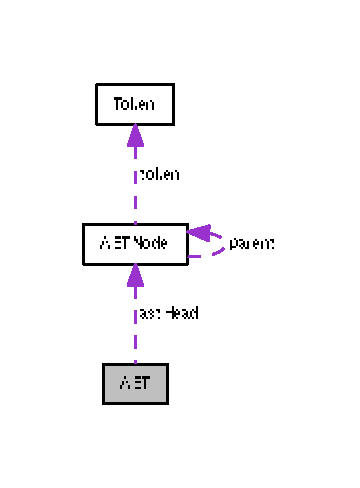
\includegraphics[width=173pt]{class_a_s_t__coll__graph}
\end{center}
\end{figure}
\subsection*{Public Member Functions}
\begin{DoxyCompactItemize}
\item 
void \hyperlink{class_a_s_t_a8fe6207ce46b87c2febdc6ebdf0be6dd}{build\+A\+S\+T} (const std\+::list$<$ \hyperlink{struct_token}{Token} $>$ \&tokens)
\item 
\hyperlink{class_a_s_t_a2daa6c636071ad4e888897a93e3dd380}{A\+S\+T} (const std\+::list$<$ \hyperlink{struct_token}{Token} $>$ \&tokens)
\item 
\hyperlink{class_a_s_t_afd378ca7cb3049d6293e8597d31d758d}{A\+S\+T} ()
\end{DoxyCompactItemize}
\subsection*{Public Attributes}
\begin{DoxyCompactItemize}
\item 
\hyperlink{struct_a_s_t_node}{A\+S\+T\+Node} \hyperlink{class_a_s_t_aaa30ec872fa91242f5c9cb7a5041b307}{ast\+Head}
\end{DoxyCompactItemize}
\subsection*{Friends}
\begin{DoxyCompactItemize}
\item 
std\+::ostream \& \hyperlink{class_a_s_t_a92b9f335ac976192dab86fc6b59d357b}{operator$<$$<$} (std\+::ostream \&o, const \hyperlink{class_a_s_t}{A\+S\+T} \&ast)
\end{DoxyCompactItemize}


\subsection{Detailed Description}


Definition at line 21 of file ast.\+hpp.



\subsection{Constructor \& Destructor Documentation}
\hypertarget{class_a_s_t_a2daa6c636071ad4e888897a93e3dd380}{}\index{A\+S\+T@{A\+S\+T}!A\+S\+T@{A\+S\+T}}
\index{A\+S\+T@{A\+S\+T}!A\+S\+T@{A\+S\+T}}
\subsubsection[{A\+S\+T}]{\setlength{\rightskip}{0pt plus 5cm}A\+S\+T\+::\+A\+S\+T (
\begin{DoxyParamCaption}
\item[{const std\+::list$<$ {\bf Token} $>$ \&}]{tokens}
\end{DoxyParamCaption}
)}\label{class_a_s_t_a2daa6c636071ad4e888897a93e3dd380}


Definition at line 25 of file ast.\+cpp.

\hypertarget{class_a_s_t_afd378ca7cb3049d6293e8597d31d758d}{}\index{A\+S\+T@{A\+S\+T}!A\+S\+T@{A\+S\+T}}
\index{A\+S\+T@{A\+S\+T}!A\+S\+T@{A\+S\+T}}
\subsubsection[{A\+S\+T}]{\setlength{\rightskip}{0pt plus 5cm}A\+S\+T\+::\+A\+S\+T (
\begin{DoxyParamCaption}
{}
\end{DoxyParamCaption}
)}\label{class_a_s_t_afd378ca7cb3049d6293e8597d31d758d}


Definition at line 20 of file ast.\+cpp.



\subsection{Member Function Documentation}
\hypertarget{class_a_s_t_a8fe6207ce46b87c2febdc6ebdf0be6dd}{}\index{A\+S\+T@{A\+S\+T}!build\+A\+S\+T@{build\+A\+S\+T}}
\index{build\+A\+S\+T@{build\+A\+S\+T}!A\+S\+T@{A\+S\+T}}
\subsubsection[{build\+A\+S\+T}]{\setlength{\rightskip}{0pt plus 5cm}void A\+S\+T\+::build\+A\+S\+T (
\begin{DoxyParamCaption}
\item[{const std\+::list$<$ {\bf Token} $>$ \&}]{tokens}
\end{DoxyParamCaption}
)}\label{class_a_s_t_a8fe6207ce46b87c2febdc6ebdf0be6dd}


Definition at line 31 of file ast.\+cpp.



\subsection{Friends And Related Function Documentation}
\hypertarget{class_a_s_t_a92b9f335ac976192dab86fc6b59d357b}{}\index{A\+S\+T@{A\+S\+T}!operator$<$$<$@{operator$<$$<$}}
\index{operator$<$$<$@{operator$<$$<$}!A\+S\+T@{A\+S\+T}}
\subsubsection[{operator$<$$<$}]{\setlength{\rightskip}{0pt plus 5cm}std\+::ostream\& operator$<$$<$ (
\begin{DoxyParamCaption}
\item[{std\+::ostream \&}]{o, }
\item[{const {\bf A\+S\+T} \&}]{ast}
\end{DoxyParamCaption}
)\hspace{0.3cm}{\ttfamily [friend]}}\label{class_a_s_t_a92b9f335ac976192dab86fc6b59d357b}


Definition at line 77 of file ast.\+cpp.



\subsection{Member Data Documentation}
\hypertarget{class_a_s_t_aaa30ec872fa91242f5c9cb7a5041b307}{}\index{A\+S\+T@{A\+S\+T}!ast\+Head@{ast\+Head}}
\index{ast\+Head@{ast\+Head}!A\+S\+T@{A\+S\+T}}
\subsubsection[{ast\+Head}]{\setlength{\rightskip}{0pt plus 5cm}{\bf A\+S\+T\+Node} A\+S\+T\+::ast\+Head}\label{class_a_s_t_aaa30ec872fa91242f5c9cb7a5041b307}


Definition at line 24 of file ast.\+hpp.



The documentation for this class was generated from the following files\+:\begin{DoxyCompactItemize}
\item 
\hyperlink{ast_8hpp}{ast.\+hpp}\item 
\hyperlink{ast_8cpp}{ast.\+cpp}\end{DoxyCompactItemize}

\hypertarget{struct_a_s_t_node}{}\section{A\+S\+T\+Node Struct Reference}
\label{struct_a_s_t_node}\index{A\+S\+T\+Node@{A\+S\+T\+Node}}


{\ttfamily \#include $<$ast.\+hpp$>$}



Collaboration diagram for A\+S\+T\+Node\+:\nopagebreak
\begin{figure}[H]
\begin{center}
\leavevmode
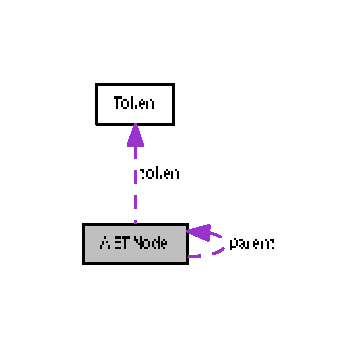
\includegraphics[width=173pt]{struct_a_s_t_node__coll__graph}
\end{center}
\end{figure}
\subsection*{Public Member Functions}
\begin{DoxyCompactItemize}
\item 
\hyperlink{struct_a_s_t_node}{A\+S\+T\+Node} $\ast$ \hyperlink{struct_a_s_t_node_adbcbd09d75a8056a48e9e9071ad8fa3e}{add} (const \hyperlink{struct_a_s_t_node}{A\+S\+T\+Node} \&node)
\item 
void \hyperlink{struct_a_s_t_node_a5198921818aa511746856219cec0b637}{remove} ()
\end{DoxyCompactItemize}
\subsection*{Public Attributes}
\begin{DoxyCompactItemize}
\item 
\hyperlink{ast_8hpp_acac9cbaeea226ed297804c012dc12b16}{Node\+Type} \hyperlink{struct_a_s_t_node_a34086f3bc5af008f08f255c8ec57ba21}{type}
\item 
\hyperlink{struct_token}{Token} \hyperlink{struct_a_s_t_node_a99c0fc8e2fe4c99fbe85d0d195cfab57}{token}
\item 
\hyperlink{struct_a_s_t_node}{A\+S\+T\+Node} $\ast$ \hyperlink{struct_a_s_t_node_aaa1e479bfeb485d93a4866f9c2daf171}{parent}
\item 
std\+::list$<$ \hyperlink{struct_a_s_t_node}{A\+S\+T\+Node} $\ast$ $>$ \hyperlink{struct_a_s_t_node_ab50690af3aacf5c7dbd0440505fd5595}{ch}
\end{DoxyCompactItemize}


\subsection{Detailed Description}


Definition at line 8 of file ast.\+hpp.



\subsection{Member Function Documentation}
\hypertarget{struct_a_s_t_node_adbcbd09d75a8056a48e9e9071ad8fa3e}{}\index{A\+S\+T\+Node@{A\+S\+T\+Node}!add@{add}}
\index{add@{add}!A\+S\+T\+Node@{A\+S\+T\+Node}}
\subsubsection[{add}]{\setlength{\rightskip}{0pt plus 5cm}{\bf A\+S\+T\+Node} $\ast$ A\+S\+T\+Node\+::add (
\begin{DoxyParamCaption}
\item[{const {\bf A\+S\+T\+Node} \&}]{node}
\end{DoxyParamCaption}
)}\label{struct_a_s_t_node_adbcbd09d75a8056a48e9e9071ad8fa3e}


Definition at line 7 of file ast.\+cpp.

\hypertarget{struct_a_s_t_node_a5198921818aa511746856219cec0b637}{}\index{A\+S\+T\+Node@{A\+S\+T\+Node}!remove@{remove}}
\index{remove@{remove}!A\+S\+T\+Node@{A\+S\+T\+Node}}
\subsubsection[{remove}]{\setlength{\rightskip}{0pt plus 5cm}void A\+S\+T\+Node\+::remove (
\begin{DoxyParamCaption}
{}
\end{DoxyParamCaption}
)}\label{struct_a_s_t_node_a5198921818aa511746856219cec0b637}


Definition at line 14 of file ast.\+cpp.



\subsection{Member Data Documentation}
\hypertarget{struct_a_s_t_node_ab50690af3aacf5c7dbd0440505fd5595}{}\index{A\+S\+T\+Node@{A\+S\+T\+Node}!ch@{ch}}
\index{ch@{ch}!A\+S\+T\+Node@{A\+S\+T\+Node}}
\subsubsection[{ch}]{\setlength{\rightskip}{0pt plus 5cm}std\+::list$<${\bf A\+S\+T\+Node}$\ast$$>$ A\+S\+T\+Node\+::ch}\label{struct_a_s_t_node_ab50690af3aacf5c7dbd0440505fd5595}


Definition at line 13 of file ast.\+hpp.

\hypertarget{struct_a_s_t_node_aaa1e479bfeb485d93a4866f9c2daf171}{}\index{A\+S\+T\+Node@{A\+S\+T\+Node}!parent@{parent}}
\index{parent@{parent}!A\+S\+T\+Node@{A\+S\+T\+Node}}
\subsubsection[{parent}]{\setlength{\rightskip}{0pt plus 5cm}{\bf A\+S\+T\+Node}$\ast$ A\+S\+T\+Node\+::parent}\label{struct_a_s_t_node_aaa1e479bfeb485d93a4866f9c2daf171}


Definition at line 12 of file ast.\+hpp.

\hypertarget{struct_a_s_t_node_a99c0fc8e2fe4c99fbe85d0d195cfab57}{}\index{A\+S\+T\+Node@{A\+S\+T\+Node}!token@{token}}
\index{token@{token}!A\+S\+T\+Node@{A\+S\+T\+Node}}
\subsubsection[{token}]{\setlength{\rightskip}{0pt plus 5cm}{\bf Token} A\+S\+T\+Node\+::token}\label{struct_a_s_t_node_a99c0fc8e2fe4c99fbe85d0d195cfab57}


Definition at line 11 of file ast.\+hpp.

\hypertarget{struct_a_s_t_node_a34086f3bc5af008f08f255c8ec57ba21}{}\index{A\+S\+T\+Node@{A\+S\+T\+Node}!type@{type}}
\index{type@{type}!A\+S\+T\+Node@{A\+S\+T\+Node}}
\subsubsection[{type}]{\setlength{\rightskip}{0pt plus 5cm}{\bf Node\+Type} A\+S\+T\+Node\+::type}\label{struct_a_s_t_node_a34086f3bc5af008f08f255c8ec57ba21}


Definition at line 10 of file ast.\+hpp.



The documentation for this struct was generated from the following files\+:\begin{DoxyCompactItemize}
\item 
\hyperlink{ast_8hpp}{ast.\+hpp}\item 
\hyperlink{ast_8cpp}{ast.\+cpp}\end{DoxyCompactItemize}

\hypertarget{class_big_int}{}\section{Big\+Int Class Reference}
\label{class_big_int}\index{Big\+Int@{Big\+Int}}


{\ttfamily \#include $<$bigint.\+hpp$>$}

\subsection*{Public Member Functions}
\begin{DoxyCompactItemize}
\item 
\hyperlink{class_big_int_a4421e6c1883874512f1b04543dafc64a}{Big\+Int} (long long num)
\item 
\hyperlink{class_big_int_abe13ffcbf871ddb97365a73120ca0b6f}{Big\+Int} (const std\+::string \&\hyperlink{preprocessortest_8cpp_a10d1ea193b80aa2128e080646057d11c}{s})
\item 
\hyperlink{class_big_int_af677021c0987fc2a48da06837ed29c58}{Big\+Int} ()
\item 
\hyperlink{class_big_int}{Big\+Int} \& \hyperlink{class_big_int_a43652944006a9ace4fa3d8e1c0ed3213}{assign} (long long num)
\item 
\hyperlink{class_big_int}{Big\+Int} \& \hyperlink{class_big_int_acc4942cf0af7096ec328735c75f8fcfe}{assign} (const std\+::string \&\hyperlink{preprocessortest_8cpp_a10d1ea193b80aa2128e080646057d11c}{s})
\item 
\hyperlink{class_big_int}{Big\+Int} \& \hyperlink{class_big_int_a5768b8d21f3cc80a85cdea09a8769a22}{operator+=} (const \hyperlink{class_big_int}{Big\+Int} \&b)
\item 
\hyperlink{class_big_int}{Big\+Int} \& \hyperlink{class_big_int_a164befb196d794282a927e1a490bb939}{operator-\/=} (const \hyperlink{class_big_int}{Big\+Int} \&b)
\item 
\hyperlink{class_big_int}{Big\+Int} \& \hyperlink{class_big_int_a8ac25b6a719f26833ad5550496c7a31d}{operator$\ast$=} (const \hyperlink{class_big_int}{Big\+Int} \&b)
\item 
\hyperlink{class_big_int}{Big\+Int} \& \hyperlink{class_big_int_aec211c9b6e6c0cc3c018ea31d63a0c16}{operator/=} (const \hyperlink{class_big_int}{Big\+Int} \&b)
\item 
\hyperlink{class_big_int}{Big\+Int} \hyperlink{class_big_int_a468c8997e2ec45ef37d5ff32becc5818}{operator+} (const \hyperlink{class_big_int}{Big\+Int} \&b) const 
\item 
\hyperlink{class_big_int}{Big\+Int} \hyperlink{class_big_int_a64ef59813d4221635ae33f8de10f88cb}{operator-\/} (const \hyperlink{class_big_int}{Big\+Int} \&b) const 
\item 
\hyperlink{class_big_int}{Big\+Int} \hyperlink{class_big_int_aa4e3204ae4a0c81e8e33d0a848078a8d}{operator$\ast$} (const \hyperlink{class_big_int}{Big\+Int} \&b) const 
\item 
\hyperlink{class_big_int}{Big\+Int} \hyperlink{class_big_int_ab5679019b8821c01b161147495e21a4e}{operator/} (const \hyperlink{class_big_int}{Big\+Int} \&b) const 
\item 
\hyperlink{class_big_int}{Big\+Int} \hyperlink{class_big_int_a56350bc8395ed38c2afdbb4554e56b1f}{operator-\/} () const 
\item 
bool \hyperlink{class_big_int_a4631ce319f6617a43a4dc89127953ebb}{operator$>$} (const \hyperlink{class_big_int}{Big\+Int} \&b) const 
\item 
bool \hyperlink{class_big_int_a56b4522f02907f0d719809a0e81c525e}{operator$<$} (const \hyperlink{class_big_int}{Big\+Int} \&b) const 
\item 
bool \hyperlink{class_big_int_a057d936831e7a103a1830366c990602f}{operator==} (const \hyperlink{class_big_int}{Big\+Int} \&b) const 
\item 
bool \hyperlink{class_big_int_ad6a59ed7dedbe35433c1a83ca751fe88}{operator!=} (const \hyperlink{class_big_int}{Big\+Int} \&b) const 
\item 
bool \hyperlink{class_big_int_ae5bdb87103df4be652062b015a1fa653}{operator$>$=} (const \hyperlink{class_big_int}{Big\+Int} \&b) const 
\item 
bool \hyperlink{class_big_int_ada9b7b9e96bb3aad13c48637397b6f31}{operator$<$=} (const \hyperlink{class_big_int}{Big\+Int} \&b) const 
\end{DoxyCompactItemize}
\subsection*{Friends}
\begin{DoxyCompactItemize}
\item 
std\+::istream \& \hyperlink{class_big_int_abfb3d978331870b4cba82ece17354f44}{operator$>$$>$} (std\+::istream \&i, \hyperlink{class_big_int}{Big\+Int} \&b)
\item 
std\+::ostream \& \hyperlink{class_big_int_a0d8814d1177634c5e0ee08e2bbccf328}{operator$<$$<$} (std\+::ostream \&o, const \hyperlink{class_big_int}{Big\+Int} \&b)
\item 
{\footnotesize template$<$typename Compare\+Func $>$ }\\bool \hyperlink{class_big_int_a95ccae99f465fac11bf28196f62dac03}{raw\+Compare} (const \hyperlink{class_big_int}{Big\+Int} \&a, const \hyperlink{class_big_int}{Big\+Int} \&b)
\end{DoxyCompactItemize}


\subsection{Detailed Description}


Definition at line 10 of file bigint.\+hpp.



\subsection{Constructor \& Destructor Documentation}
\hypertarget{class_big_int_a4421e6c1883874512f1b04543dafc64a}{}\index{Big\+Int@{Big\+Int}!Big\+Int@{Big\+Int}}
\index{Big\+Int@{Big\+Int}!Big\+Int@{Big\+Int}}
\subsubsection[{Big\+Int}]{\setlength{\rightskip}{0pt plus 5cm}Big\+Int\+::\+Big\+Int (
\begin{DoxyParamCaption}
\item[{long long}]{num}
\end{DoxyParamCaption}
)}\label{class_big_int_a4421e6c1883874512f1b04543dafc64a}


Definition at line 19 of file bigint.\+cpp.

\hypertarget{class_big_int_abe13ffcbf871ddb97365a73120ca0b6f}{}\index{Big\+Int@{Big\+Int}!Big\+Int@{Big\+Int}}
\index{Big\+Int@{Big\+Int}!Big\+Int@{Big\+Int}}
\subsubsection[{Big\+Int}]{\setlength{\rightskip}{0pt plus 5cm}Big\+Int\+::\+Big\+Int (
\begin{DoxyParamCaption}
\item[{const std\+::string \&}]{s}
\end{DoxyParamCaption}
)}\label{class_big_int_abe13ffcbf871ddb97365a73120ca0b6f}


Definition at line 24 of file bigint.\+cpp.

\hypertarget{class_big_int_af677021c0987fc2a48da06837ed29c58}{}\index{Big\+Int@{Big\+Int}!Big\+Int@{Big\+Int}}
\index{Big\+Int@{Big\+Int}!Big\+Int@{Big\+Int}}
\subsubsection[{Big\+Int}]{\setlength{\rightskip}{0pt plus 5cm}Big\+Int\+::\+Big\+Int (
\begin{DoxyParamCaption}
{}
\end{DoxyParamCaption}
)}\label{class_big_int_af677021c0987fc2a48da06837ed29c58}


Definition at line 29 of file bigint.\+cpp.



\subsection{Member Function Documentation}
\hypertarget{class_big_int_a43652944006a9ace4fa3d8e1c0ed3213}{}\index{Big\+Int@{Big\+Int}!assign@{assign}}
\index{assign@{assign}!Big\+Int@{Big\+Int}}
\subsubsection[{assign}]{\setlength{\rightskip}{0pt plus 5cm}{\bf Big\+Int} \& Big\+Int\+::assign (
\begin{DoxyParamCaption}
\item[{long long}]{num}
\end{DoxyParamCaption}
)}\label{class_big_int_a43652944006a9ace4fa3d8e1c0ed3213}


Definition at line 34 of file bigint.\+cpp.

\hypertarget{class_big_int_acc4942cf0af7096ec328735c75f8fcfe}{}\index{Big\+Int@{Big\+Int}!assign@{assign}}
\index{assign@{assign}!Big\+Int@{Big\+Int}}
\subsubsection[{assign}]{\setlength{\rightskip}{0pt plus 5cm}{\bf Big\+Int} \& Big\+Int\+::assign (
\begin{DoxyParamCaption}
\item[{const std\+::string \&}]{s}
\end{DoxyParamCaption}
)}\label{class_big_int_acc4942cf0af7096ec328735c75f8fcfe}


Definition at line 55 of file bigint.\+cpp.

\hypertarget{class_big_int_ad6a59ed7dedbe35433c1a83ca751fe88}{}\index{Big\+Int@{Big\+Int}!operator"!=@{operator"!=}}
\index{operator"!=@{operator"!=}!Big\+Int@{Big\+Int}}
\subsubsection[{operator"!=}]{\setlength{\rightskip}{0pt plus 5cm}bool Big\+Int\+::operator!= (
\begin{DoxyParamCaption}
\item[{const {\bf Big\+Int} \&}]{b}
\end{DoxyParamCaption}
) const}\label{class_big_int_ad6a59ed7dedbe35433c1a83ca751fe88}


Definition at line 145 of file bigint.\+cpp.

\hypertarget{class_big_int_aa4e3204ae4a0c81e8e33d0a848078a8d}{}\index{Big\+Int@{Big\+Int}!operator$\ast$@{operator$\ast$}}
\index{operator$\ast$@{operator$\ast$}!Big\+Int@{Big\+Int}}
\subsubsection[{operator$\ast$}]{\setlength{\rightskip}{0pt plus 5cm}{\bf Big\+Int} Big\+Int\+::operator$\ast$ (
\begin{DoxyParamCaption}
\item[{const {\bf Big\+Int} \&}]{b}
\end{DoxyParamCaption}
) const}\label{class_big_int_aa4e3204ae4a0c81e8e33d0a848078a8d}
\hypertarget{class_big_int_a8ac25b6a719f26833ad5550496c7a31d}{}\index{Big\+Int@{Big\+Int}!operator$\ast$=@{operator$\ast$=}}
\index{operator$\ast$=@{operator$\ast$=}!Big\+Int@{Big\+Int}}
\subsubsection[{operator$\ast$=}]{\setlength{\rightskip}{0pt plus 5cm}{\bf Big\+Int}\& Big\+Int\+::operator$\ast$= (
\begin{DoxyParamCaption}
\item[{const {\bf Big\+Int} \&}]{b}
\end{DoxyParamCaption}
)}\label{class_big_int_a8ac25b6a719f26833ad5550496c7a31d}
\hypertarget{class_big_int_a468c8997e2ec45ef37d5ff32becc5818}{}\index{Big\+Int@{Big\+Int}!operator+@{operator+}}
\index{operator+@{operator+}!Big\+Int@{Big\+Int}}
\subsubsection[{operator+}]{\setlength{\rightskip}{0pt plus 5cm}{\bf Big\+Int} Big\+Int\+::operator+ (
\begin{DoxyParamCaption}
\item[{const {\bf Big\+Int} \&}]{b}
\end{DoxyParamCaption}
) const}\label{class_big_int_a468c8997e2ec45ef37d5ff32becc5818}


Definition at line 261 of file bigint.\+cpp.

\hypertarget{class_big_int_a5768b8d21f3cc80a85cdea09a8769a22}{}\index{Big\+Int@{Big\+Int}!operator+=@{operator+=}}
\index{operator+=@{operator+=}!Big\+Int@{Big\+Int}}
\subsubsection[{operator+=}]{\setlength{\rightskip}{0pt plus 5cm}{\bf Big\+Int} \& Big\+Int\+::operator+= (
\begin{DoxyParamCaption}
\item[{const {\bf Big\+Int} \&}]{b}
\end{DoxyParamCaption}
)}\label{class_big_int_a5768b8d21f3cc80a85cdea09a8769a22}


Definition at line 199 of file bigint.\+cpp.

\hypertarget{class_big_int_a64ef59813d4221635ae33f8de10f88cb}{}\index{Big\+Int@{Big\+Int}!operator-\/@{operator-\/}}
\index{operator-\/@{operator-\/}!Big\+Int@{Big\+Int}}
\subsubsection[{operator-\/}]{\setlength{\rightskip}{0pt plus 5cm}{\bf Big\+Int} Big\+Int\+::operator-\/ (
\begin{DoxyParamCaption}
\item[{const {\bf Big\+Int} \&}]{b}
\end{DoxyParamCaption}
) const}\label{class_big_int_a64ef59813d4221635ae33f8de10f88cb}


Definition at line 268 of file bigint.\+cpp.

\hypertarget{class_big_int_a56350bc8395ed38c2afdbb4554e56b1f}{}\index{Big\+Int@{Big\+Int}!operator-\/@{operator-\/}}
\index{operator-\/@{operator-\/}!Big\+Int@{Big\+Int}}
\subsubsection[{operator-\/}]{\setlength{\rightskip}{0pt plus 5cm}{\bf Big\+Int} Big\+Int\+::operator-\/ (
\begin{DoxyParamCaption}
{}
\end{DoxyParamCaption}
) const}\label{class_big_int_a56350bc8395ed38c2afdbb4554e56b1f}


Definition at line 94 of file bigint.\+cpp.

\hypertarget{class_big_int_a164befb196d794282a927e1a490bb939}{}\index{Big\+Int@{Big\+Int}!operator-\/=@{operator-\/=}}
\index{operator-\/=@{operator-\/=}!Big\+Int@{Big\+Int}}
\subsubsection[{operator-\/=}]{\setlength{\rightskip}{0pt plus 5cm}{\bf Big\+Int} \& Big\+Int\+::operator-\/= (
\begin{DoxyParamCaption}
\item[{const {\bf Big\+Int} \&}]{b}
\end{DoxyParamCaption}
)}\label{class_big_int_a164befb196d794282a927e1a490bb939}


Definition at line 232 of file bigint.\+cpp.

\hypertarget{class_big_int_ab5679019b8821c01b161147495e21a4e}{}\index{Big\+Int@{Big\+Int}!operator/@{operator/}}
\index{operator/@{operator/}!Big\+Int@{Big\+Int}}
\subsubsection[{operator/}]{\setlength{\rightskip}{0pt plus 5cm}{\bf Big\+Int} Big\+Int\+::operator/ (
\begin{DoxyParamCaption}
\item[{const {\bf Big\+Int} \&}]{b}
\end{DoxyParamCaption}
) const}\label{class_big_int_ab5679019b8821c01b161147495e21a4e}
\hypertarget{class_big_int_aec211c9b6e6c0cc3c018ea31d63a0c16}{}\index{Big\+Int@{Big\+Int}!operator/=@{operator/=}}
\index{operator/=@{operator/=}!Big\+Int@{Big\+Int}}
\subsubsection[{operator/=}]{\setlength{\rightskip}{0pt plus 5cm}{\bf Big\+Int}\& Big\+Int\+::operator/= (
\begin{DoxyParamCaption}
\item[{const {\bf Big\+Int} \&}]{b}
\end{DoxyParamCaption}
)}\label{class_big_int_aec211c9b6e6c0cc3c018ea31d63a0c16}
\hypertarget{class_big_int_a56b4522f02907f0d719809a0e81c525e}{}\index{Big\+Int@{Big\+Int}!operator$<$@{operator$<$}}
\index{operator$<$@{operator$<$}!Big\+Int@{Big\+Int}}
\subsubsection[{operator$<$}]{\setlength{\rightskip}{0pt plus 5cm}bool Big\+Int\+::operator$<$ (
\begin{DoxyParamCaption}
\item[{const {\bf Big\+Int} \&}]{b}
\end{DoxyParamCaption}
) const}\label{class_big_int_a56b4522f02907f0d719809a0e81c525e}


Definition at line 123 of file bigint.\+cpp.

\hypertarget{class_big_int_ada9b7b9e96bb3aad13c48637397b6f31}{}\index{Big\+Int@{Big\+Int}!operator$<$=@{operator$<$=}}
\index{operator$<$=@{operator$<$=}!Big\+Int@{Big\+Int}}
\subsubsection[{operator$<$=}]{\setlength{\rightskip}{0pt plus 5cm}bool Big\+Int\+::operator$<$= (
\begin{DoxyParamCaption}
\item[{const {\bf Big\+Int} \&}]{b}
\end{DoxyParamCaption}
) const}\label{class_big_int_ada9b7b9e96bb3aad13c48637397b6f31}


Definition at line 155 of file bigint.\+cpp.

\hypertarget{class_big_int_a057d936831e7a103a1830366c990602f}{}\index{Big\+Int@{Big\+Int}!operator==@{operator==}}
\index{operator==@{operator==}!Big\+Int@{Big\+Int}}
\subsubsection[{operator==}]{\setlength{\rightskip}{0pt plus 5cm}bool Big\+Int\+::operator== (
\begin{DoxyParamCaption}
\item[{const {\bf Big\+Int} \&}]{b}
\end{DoxyParamCaption}
) const}\label{class_big_int_a057d936831e7a103a1830366c990602f}


Definition at line 137 of file bigint.\+cpp.

\hypertarget{class_big_int_a4631ce319f6617a43a4dc89127953ebb}{}\index{Big\+Int@{Big\+Int}!operator$>$@{operator$>$}}
\index{operator$>$@{operator$>$}!Big\+Int@{Big\+Int}}
\subsubsection[{operator$>$}]{\setlength{\rightskip}{0pt plus 5cm}bool Big\+Int\+::operator$>$ (
\begin{DoxyParamCaption}
\item[{const {\bf Big\+Int} \&}]{b}
\end{DoxyParamCaption}
) const}\label{class_big_int_a4631ce319f6617a43a4dc89127953ebb}


Definition at line 132 of file bigint.\+cpp.

\hypertarget{class_big_int_ae5bdb87103df4be652062b015a1fa653}{}\index{Big\+Int@{Big\+Int}!operator$>$=@{operator$>$=}}
\index{operator$>$=@{operator$>$=}!Big\+Int@{Big\+Int}}
\subsubsection[{operator$>$=}]{\setlength{\rightskip}{0pt plus 5cm}bool Big\+Int\+::operator$>$= (
\begin{DoxyParamCaption}
\item[{const {\bf Big\+Int} \&}]{b}
\end{DoxyParamCaption}
) const}\label{class_big_int_ae5bdb87103df4be652062b015a1fa653}


Definition at line 150 of file bigint.\+cpp.



\subsection{Friends And Related Function Documentation}
\hypertarget{class_big_int_a0d8814d1177634c5e0ee08e2bbccf328}{}\index{Big\+Int@{Big\+Int}!operator$<$$<$@{operator$<$$<$}}
\index{operator$<$$<$@{operator$<$$<$}!Big\+Int@{Big\+Int}}
\subsubsection[{operator$<$$<$}]{\setlength{\rightskip}{0pt plus 5cm}std\+::ostream\& operator$<$$<$ (
\begin{DoxyParamCaption}
\item[{std\+::ostream \&}]{o, }
\item[{const {\bf Big\+Int} \&}]{b}
\end{DoxyParamCaption}
)\hspace{0.3cm}{\ttfamily [friend]}}\label{class_big_int_a0d8814d1177634c5e0ee08e2bbccf328}


Definition at line 245 of file bigint.\+cpp.

\hypertarget{class_big_int_abfb3d978331870b4cba82ece17354f44}{}\index{Big\+Int@{Big\+Int}!operator$>$$>$@{operator$>$$>$}}
\index{operator$>$$>$@{operator$>$$>$}!Big\+Int@{Big\+Int}}
\subsubsection[{operator$>$$>$}]{\setlength{\rightskip}{0pt plus 5cm}std\+::istream\& operator$>$$>$ (
\begin{DoxyParamCaption}
\item[{std\+::istream \&}]{i, }
\item[{{\bf Big\+Int} \&}]{b}
\end{DoxyParamCaption}
)\hspace{0.3cm}{\ttfamily [friend]}}\label{class_big_int_abfb3d978331870b4cba82ece17354f44}


Definition at line 237 of file bigint.\+cpp.

\hypertarget{class_big_int_a95ccae99f465fac11bf28196f62dac03}{}\index{Big\+Int@{Big\+Int}!raw\+Compare@{raw\+Compare}}
\index{raw\+Compare@{raw\+Compare}!Big\+Int@{Big\+Int}}
\subsubsection[{raw\+Compare}]{\setlength{\rightskip}{0pt plus 5cm}template$<$typename Compare\+Func $>$ bool raw\+Compare (
\begin{DoxyParamCaption}
\item[{const {\bf Big\+Int} \&}]{a, }
\item[{const {\bf Big\+Int} \&}]{b}
\end{DoxyParamCaption}
)\hspace{0.3cm}{\ttfamily [friend]}}\label{class_big_int_a95ccae99f465fac11bf28196f62dac03}


Definition at line 103 of file bigint.\+cpp.



The documentation for this class was generated from the following files\+:\begin{DoxyCompactItemize}
\item 
utility/\hyperlink{bigint_8hpp}{bigint.\+hpp}\item 
utility/\hyperlink{bigint_8cpp}{bigint.\+cpp}\end{DoxyCompactItemize}

\hypertarget{class_op_minus_a_s_t_parser}{}\section{Op\+Minus\+A\+S\+T\+Parser Class Reference}
\label{class_op_minus_a_s_t_parser}\index{Op\+Minus\+A\+S\+T\+Parser@{Op\+Minus\+A\+S\+T\+Parser}}


{\ttfamily \#include $<$opminus.\+hpp$>$}

\subsection*{Public Member Functions}
\begin{DoxyCompactItemize}
\item 
bool \hyperlink{class_op_minus_a_s_t_parser_ac9ffe930b5614d5708a3d8ad9bc6f3d6}{judge} (const \hyperlink{struct_a_s_t_node}{A\+S\+T\+Node} \&astnode, const \hyperlink{class_parsers_helper}{Parsers\+Helper} \&parser\+Helper)
\item 
void \hyperlink{class_op_minus_a_s_t_parser_a7e3739bcb6a04afc33d6f2e2f523a2f0}{parse} (\hyperlink{struct_a_s_t_node}{A\+S\+T\+Node} \&astnode, \hyperlink{class_parsers_helper}{Parsers\+Helper} \&parser\+Helper)
\end{DoxyCompactItemize}


\subsection{Detailed Description}


Definition at line 6 of file opminus.\+hpp.



\subsection{Member Function Documentation}
\hypertarget{class_op_minus_a_s_t_parser_ac9ffe930b5614d5708a3d8ad9bc6f3d6}{}\index{Op\+Minus\+A\+S\+T\+Parser@{Op\+Minus\+A\+S\+T\+Parser}!judge@{judge}}
\index{judge@{judge}!Op\+Minus\+A\+S\+T\+Parser@{Op\+Minus\+A\+S\+T\+Parser}}
\subsubsection[{judge}]{\setlength{\rightskip}{0pt plus 5cm}bool Op\+Minus\+A\+S\+T\+Parser\+::judge (
\begin{DoxyParamCaption}
\item[{const {\bf A\+S\+T\+Node} \&}]{astnode, }
\item[{const {\bf Parsers\+Helper} \&}]{parser\+Helper}
\end{DoxyParamCaption}
)}\label{class_op_minus_a_s_t_parser_ac9ffe930b5614d5708a3d8ad9bc6f3d6}


Definition at line 11 of file opminus.\+cpp.

\hypertarget{class_op_minus_a_s_t_parser_a7e3739bcb6a04afc33d6f2e2f523a2f0}{}\index{Op\+Minus\+A\+S\+T\+Parser@{Op\+Minus\+A\+S\+T\+Parser}!parse@{parse}}
\index{parse@{parse}!Op\+Minus\+A\+S\+T\+Parser@{Op\+Minus\+A\+S\+T\+Parser}}
\subsubsection[{parse}]{\setlength{\rightskip}{0pt plus 5cm}void Op\+Minus\+A\+S\+T\+Parser\+::parse (
\begin{DoxyParamCaption}
\item[{{\bf A\+S\+T\+Node} \&}]{astnode, }
\item[{{\bf Parsers\+Helper} \&}]{parser\+Helper}
\end{DoxyParamCaption}
)}\label{class_op_minus_a_s_t_parser_a7e3739bcb6a04afc33d6f2e2f523a2f0}


Definition at line 16 of file opminus.\+cpp.



The documentation for this class was generated from the following files\+:\begin{DoxyCompactItemize}
\item 
parsers/\hyperlink{opminus_8hpp}{opminus.\+hpp}\item 
parsers/\hyperlink{opminus_8cpp}{opminus.\+cpp}\end{DoxyCompactItemize}

\hypertarget{class_op_plus_a_s_t_parser}{}\section{Op\+Plus\+A\+S\+T\+Parser Class Reference}
\label{class_op_plus_a_s_t_parser}\index{Op\+Plus\+A\+S\+T\+Parser@{Op\+Plus\+A\+S\+T\+Parser}}


{\ttfamily \#include $<$opplus.\+hpp$>$}

\subsection*{Public Member Functions}
\begin{DoxyCompactItemize}
\item 
bool \hyperlink{class_op_plus_a_s_t_parser_a7275117187eae6fb59ebfb58e988b863}{judge} (const \hyperlink{struct_a_s_t_node}{A\+S\+T\+Node} \&astnode, const \hyperlink{class_parsers_helper}{Parsers\+Helper} \&parser\+Helper)
\item 
void \hyperlink{class_op_plus_a_s_t_parser_afa55f86d5fa18f2e9d0df1753db28c74}{parse} (\hyperlink{struct_a_s_t_node}{A\+S\+T\+Node} \&astnode, \hyperlink{class_parsers_helper}{Parsers\+Helper} \&parser\+Helper)
\end{DoxyCompactItemize}


\subsection{Detailed Description}


Definition at line 5 of file opplus.\+hpp.



\subsection{Member Function Documentation}
\hypertarget{class_op_plus_a_s_t_parser_a7275117187eae6fb59ebfb58e988b863}{}\index{Op\+Plus\+A\+S\+T\+Parser@{Op\+Plus\+A\+S\+T\+Parser}!judge@{judge}}
\index{judge@{judge}!Op\+Plus\+A\+S\+T\+Parser@{Op\+Plus\+A\+S\+T\+Parser}}
\subsubsection[{judge}]{\setlength{\rightskip}{0pt plus 5cm}bool Op\+Plus\+A\+S\+T\+Parser\+::judge (
\begin{DoxyParamCaption}
\item[{const {\bf A\+S\+T\+Node} \&}]{astnode, }
\item[{const {\bf Parsers\+Helper} \&}]{parser\+Helper}
\end{DoxyParamCaption}
)}\label{class_op_plus_a_s_t_parser_a7275117187eae6fb59ebfb58e988b863}


Definition at line 9 of file opplus.\+cpp.

\hypertarget{class_op_plus_a_s_t_parser_afa55f86d5fa18f2e9d0df1753db28c74}{}\index{Op\+Plus\+A\+S\+T\+Parser@{Op\+Plus\+A\+S\+T\+Parser}!parse@{parse}}
\index{parse@{parse}!Op\+Plus\+A\+S\+T\+Parser@{Op\+Plus\+A\+S\+T\+Parser}}
\subsubsection[{parse}]{\setlength{\rightskip}{0pt plus 5cm}void Op\+Plus\+A\+S\+T\+Parser\+::parse (
\begin{DoxyParamCaption}
\item[{{\bf A\+S\+T\+Node} \&}]{astnode, }
\item[{{\bf Parsers\+Helper} \&}]{parser\+Helper}
\end{DoxyParamCaption}
)}\label{class_op_plus_a_s_t_parser_afa55f86d5fa18f2e9d0df1753db28c74}


Definition at line 15 of file opplus.\+cpp.



The documentation for this class was generated from the following files\+:\begin{DoxyCompactItemize}
\item 
parsers/\hyperlink{opplus_8hpp}{opplus.\+hpp}\item 
parsers/\hyperlink{opplus_8cpp}{opplus.\+cpp}\end{DoxyCompactItemize}

\hypertarget{class_parsers_helper}{}\section{Parsers\+Helper Class Reference}
\label{class_parsers_helper}\index{Parsers\+Helper@{Parsers\+Helper}}


{\ttfamily \#include $<$all.\+hpp$>$}

\subsection*{Public Member Functions}
\begin{DoxyCompactItemize}
\item 
\hyperlink{class_parsers_helper_a4abfe81f7251ffe4635c2ed2e482645d}{Parsers\+Helper} ()
\item 
void \hyperlink{class_parsers_helper_a21ce6213ee29e0459dd655c6803db00b}{parse} (\hyperlink{ast_8hpp_ab65291a3ef1ea9ec8e3d396783b77e46}{P\+A\+S\+T\+Node} astnode)
\item 
{\footnotesize template$<$typename T $>$ }\\void \hyperlink{class_parsers_helper_affae95c60593e3a8154f29e7b10daf17}{operator()} (T \&)
\end{DoxyCompactItemize}
\subsection*{Private Types}
\begin{DoxyCompactItemize}
\item 
enum \{ \hyperlink{class_parsers_helper_ac5239b5c4a61b2f239f668b738f613bea11c61fd76dd1cc499d0a82c995b29009}{Construct}, 
\hyperlink{class_parsers_helper_ac5239b5c4a61b2f239f668b738f613beae4bcb2b09e1ae01be6741b0d5dff5252}{Parse}
 \}
\end{DoxyCompactItemize}
\subsection*{Private Attributes}
\begin{DoxyCompactItemize}
\item 
std\+::shared\+\_\+ptr$<$ std\+::vector$<$ \hyperlink{parsers_2all_8hpp_abe36ed7c3b8a2eebe6d943c84fe72b9c}{Parser\+Type} $>$ $>$ \hyperlink{class_parsers_helper_a1c30abdf7ce5ad7d5e67237f88f18223}{a}
\item 
int \hyperlink{class_parsers_helper_a51c199f259d9aadab7d02681c9e57c49}{cur}
\item 
\hyperlink{ast_8hpp_ab65291a3ef1ea9ec8e3d396783b77e46}{P\+A\+S\+T\+Node} \hyperlink{class_parsers_helper_a37f84842cb32827280bff1663f43d750}{nod}
\item 
bool \hyperlink{class_parsers_helper_a88e598a10d698b0962efa12ee6121436}{ok}
\item 
enum Parsers\+Helper\+:: \{ ... \}  \hyperlink{class_parsers_helper_a268b5522cce719a0c28d3e48d9b5cc04}{state}
\end{DoxyCompactItemize}


\subsection{Detailed Description}


Definition at line 34 of file all.\+hpp.



\subsection{Member Enumeration Documentation}
\hypertarget{class_parsers_helper_ac5239b5c4a61b2f239f668b738f613be}{}\subsubsection[{anonymous enum}]{\setlength{\rightskip}{0pt plus 5cm}anonymous enum\hspace{0.3cm}{\ttfamily [private]}}\label{class_parsers_helper_ac5239b5c4a61b2f239f668b738f613be}
\begin{Desc}
\item[Enumerator]\par
\begin{description}
\index{Construct@{Construct}!Parsers\+Helper@{Parsers\+Helper}}\index{Parsers\+Helper@{Parsers\+Helper}!Construct@{Construct}}\item[{\em 
\hypertarget{class_parsers_helper_ac5239b5c4a61b2f239f668b738f613bea11c61fd76dd1cc499d0a82c995b29009}{}Construct\label{class_parsers_helper_ac5239b5c4a61b2f239f668b738f613bea11c61fd76dd1cc499d0a82c995b29009}
}]\index{Parse@{Parse}!Parsers\+Helper@{Parsers\+Helper}}\index{Parsers\+Helper@{Parsers\+Helper}!Parse@{Parse}}\item[{\em 
\hypertarget{class_parsers_helper_ac5239b5c4a61b2f239f668b738f613beae4bcb2b09e1ae01be6741b0d5dff5252}{}Parse\label{class_parsers_helper_ac5239b5c4a61b2f239f668b738f613beae4bcb2b09e1ae01be6741b0d5dff5252}
}]\end{description}
\end{Desc}


Definition at line 40 of file all.\+hpp.



\subsection{Constructor \& Destructor Documentation}
\hypertarget{class_parsers_helper_a4abfe81f7251ffe4635c2ed2e482645d}{}\index{Parsers\+Helper@{Parsers\+Helper}!Parsers\+Helper@{Parsers\+Helper}}
\index{Parsers\+Helper@{Parsers\+Helper}!Parsers\+Helper@{Parsers\+Helper}}
\subsubsection[{Parsers\+Helper}]{\setlength{\rightskip}{0pt plus 5cm}Parsers\+Helper\+::\+Parsers\+Helper (
\begin{DoxyParamCaption}
{}
\end{DoxyParamCaption}
)}\label{class_parsers_helper_a4abfe81f7251ffe4635c2ed2e482645d}


Definition at line 7 of file all.\+cpp.



\subsection{Member Function Documentation}
\hypertarget{class_parsers_helper_affae95c60593e3a8154f29e7b10daf17}{}\index{Parsers\+Helper@{Parsers\+Helper}!operator()@{operator()}}
\index{operator()@{operator()}!Parsers\+Helper@{Parsers\+Helper}}
\subsubsection[{operator()}]{\setlength{\rightskip}{0pt plus 5cm}template$<$typename T $>$ void Parsers\+Helper\+::operator() (
\begin{DoxyParamCaption}
\item[{T \&}]{}
\end{DoxyParamCaption}
)}\label{class_parsers_helper_affae95c60593e3a8154f29e7b10daf17}


Definition at line 48 of file all.\+hpp.

\hypertarget{class_parsers_helper_a21ce6213ee29e0459dd655c6803db00b}{}\index{Parsers\+Helper@{Parsers\+Helper}!parse@{parse}}
\index{parse@{parse}!Parsers\+Helper@{Parsers\+Helper}}
\subsubsection[{parse}]{\setlength{\rightskip}{0pt plus 5cm}void Parsers\+Helper\+::parse (
\begin{DoxyParamCaption}
\item[{{\bf P\+A\+S\+T\+Node}}]{astnode}
\end{DoxyParamCaption}
)}\label{class_parsers_helper_a21ce6213ee29e0459dd655c6803db00b}


Definition at line 15 of file all.\+cpp.



\subsection{Member Data Documentation}
\hypertarget{class_parsers_helper_a1c30abdf7ce5ad7d5e67237f88f18223}{}\index{Parsers\+Helper@{Parsers\+Helper}!a@{a}}
\index{a@{a}!Parsers\+Helper@{Parsers\+Helper}}
\subsubsection[{a}]{\setlength{\rightskip}{0pt plus 5cm}std\+::shared\+\_\+ptr$<$std\+::vector$<${\bf Parser\+Type}$>$ $>$ Parsers\+Helper\+::a\hspace{0.3cm}{\ttfamily [private]}}\label{class_parsers_helper_a1c30abdf7ce5ad7d5e67237f88f18223}


Definition at line 36 of file all.\+hpp.

\hypertarget{class_parsers_helper_a51c199f259d9aadab7d02681c9e57c49}{}\index{Parsers\+Helper@{Parsers\+Helper}!cur@{cur}}
\index{cur@{cur}!Parsers\+Helper@{Parsers\+Helper}}
\subsubsection[{cur}]{\setlength{\rightskip}{0pt plus 5cm}int Parsers\+Helper\+::cur\hspace{0.3cm}{\ttfamily [private]}}\label{class_parsers_helper_a51c199f259d9aadab7d02681c9e57c49}


Definition at line 37 of file all.\+hpp.

\hypertarget{class_parsers_helper_a37f84842cb32827280bff1663f43d750}{}\index{Parsers\+Helper@{Parsers\+Helper}!nod@{nod}}
\index{nod@{nod}!Parsers\+Helper@{Parsers\+Helper}}
\subsubsection[{nod}]{\setlength{\rightskip}{0pt plus 5cm}{\bf P\+A\+S\+T\+Node} Parsers\+Helper\+::nod\hspace{0.3cm}{\ttfamily [private]}}\label{class_parsers_helper_a37f84842cb32827280bff1663f43d750}


Definition at line 38 of file all.\+hpp.

\hypertarget{class_parsers_helper_a88e598a10d698b0962efa12ee6121436}{}\index{Parsers\+Helper@{Parsers\+Helper}!ok@{ok}}
\index{ok@{ok}!Parsers\+Helper@{Parsers\+Helper}}
\subsubsection[{ok}]{\setlength{\rightskip}{0pt plus 5cm}bool Parsers\+Helper\+::ok\hspace{0.3cm}{\ttfamily [private]}}\label{class_parsers_helper_a88e598a10d698b0962efa12ee6121436}


Definition at line 39 of file all.\+hpp.

\hypertarget{class_parsers_helper_a268b5522cce719a0c28d3e48d9b5cc04}{}\index{Parsers\+Helper@{Parsers\+Helper}!state@{state}}
\index{state@{state}!Parsers\+Helper@{Parsers\+Helper}}
\subsubsection[{state}]{\setlength{\rightskip}{0pt plus 5cm}enum \{ ... \}   Parsers\+Helper\+::state\hspace{0.3cm}{\ttfamily [private]}}\label{class_parsers_helper_a268b5522cce719a0c28d3e48d9b5cc04}


The documentation for this class was generated from the following files\+:\begin{DoxyCompactItemize}
\item 
parsers/\hyperlink{parsers_2all_8hpp}{all.\+hpp}\item 
parsers/\hyperlink{parsers_2all_8cpp}{all.\+cpp}\end{DoxyCompactItemize}

\hypertarget{struct_parser_visitor}{}\section{Parser\+Visitor Struct Reference}
\label{struct_parser_visitor}\index{Parser\+Visitor@{Parser\+Visitor}}


{\ttfamily \#include $<$all.\+hpp$>$}

\subsection*{Public Member Functions}
\begin{DoxyCompactItemize}
\item 
{\footnotesize template$<$typename T $>$ }\\void \hyperlink{struct_parser_visitor_aa5a5df33bf6193a75c72eb2eeb492429}{operator()} (T \&)
\item 
void \hyperlink{struct_parser_visitor_a241c6d04c5a0e736ee477d5d93af8ac7}{parse} (const string \&token\+\_\+)
\end{DoxyCompactItemize}
\subsection*{Public Attributes}
\begin{DoxyCompactItemize}
\item 
bool \hyperlink{struct_parser_visitor_af5c2d247a1ec646aded499e01ca71553}{ok}
\item 
std\+::string \hyperlink{struct_parser_visitor_a75c39e97645b48c171b9912440aa9ca2}{token}
\item 
\hyperlink{types_2arch_8hpp_aa520fbf142ba1e7e659590c07da31921}{Token\+Type} \hyperlink{struct_parser_visitor_acaa4d8ca1662ec314ae2a8f048f6aca3}{token\+Type}
\item 
\hyperlink{types_2all_8hpp_a58b4bafc5e94cba5e42b944a85b061db}{Info\+Types} \hyperlink{struct_parser_visitor_a44159efad79cb74d477675367d8dcc3f}{info}
\end{DoxyCompactItemize}


\subsection{Detailed Description}


Definition at line 48 of file all.\+hpp.



\subsection{Member Function Documentation}
\hypertarget{struct_parser_visitor_aa5a5df33bf6193a75c72eb2eeb492429}{}\index{Parser\+Visitor@{Parser\+Visitor}!operator()@{operator()}}
\index{operator()@{operator()}!Parser\+Visitor@{Parser\+Visitor}}
\subsubsection[{operator()}]{\setlength{\rightskip}{0pt plus 5cm}template$<$typename T $>$ void Parser\+Visitor\+::operator() (
\begin{DoxyParamCaption}
\item[{T \&}]{}
\end{DoxyParamCaption}
)}\label{struct_parser_visitor_aa5a5df33bf6193a75c72eb2eeb492429}


Definition at line 59 of file all.\+hpp.

\hypertarget{struct_parser_visitor_a241c6d04c5a0e736ee477d5d93af8ac7}{}\index{Parser\+Visitor@{Parser\+Visitor}!parse@{parse}}
\index{parse@{parse}!Parser\+Visitor@{Parser\+Visitor}}
\subsubsection[{parse}]{\setlength{\rightskip}{0pt plus 5cm}void Parser\+Visitor\+::parse (
\begin{DoxyParamCaption}
\item[{const string \&}]{token\+\_\+}
\end{DoxyParamCaption}
)}\label{struct_parser_visitor_a241c6d04c5a0e736ee477d5d93af8ac7}


Definition at line 3 of file all.\+cpp.



\subsection{Member Data Documentation}
\hypertarget{struct_parser_visitor_a44159efad79cb74d477675367d8dcc3f}{}\index{Parser\+Visitor@{Parser\+Visitor}!info@{info}}
\index{info@{info}!Parser\+Visitor@{Parser\+Visitor}}
\subsubsection[{info}]{\setlength{\rightskip}{0pt plus 5cm}{\bf Info\+Types} Parser\+Visitor\+::info}\label{struct_parser_visitor_a44159efad79cb74d477675367d8dcc3f}


Definition at line 53 of file all.\+hpp.

\hypertarget{struct_parser_visitor_af5c2d247a1ec646aded499e01ca71553}{}\index{Parser\+Visitor@{Parser\+Visitor}!ok@{ok}}
\index{ok@{ok}!Parser\+Visitor@{Parser\+Visitor}}
\subsubsection[{ok}]{\setlength{\rightskip}{0pt plus 5cm}bool Parser\+Visitor\+::ok}\label{struct_parser_visitor_af5c2d247a1ec646aded499e01ca71553}


Definition at line 50 of file all.\+hpp.

\hypertarget{struct_parser_visitor_a75c39e97645b48c171b9912440aa9ca2}{}\index{Parser\+Visitor@{Parser\+Visitor}!token@{token}}
\index{token@{token}!Parser\+Visitor@{Parser\+Visitor}}
\subsubsection[{token}]{\setlength{\rightskip}{0pt plus 5cm}std\+::string Parser\+Visitor\+::token}\label{struct_parser_visitor_a75c39e97645b48c171b9912440aa9ca2}


Definition at line 51 of file all.\+hpp.

\hypertarget{struct_parser_visitor_acaa4d8ca1662ec314ae2a8f048f6aca3}{}\index{Parser\+Visitor@{Parser\+Visitor}!token\+Type@{token\+Type}}
\index{token\+Type@{token\+Type}!Parser\+Visitor@{Parser\+Visitor}}
\subsubsection[{token\+Type}]{\setlength{\rightskip}{0pt plus 5cm}{\bf Token\+Type} Parser\+Visitor\+::token\+Type}\label{struct_parser_visitor_acaa4d8ca1662ec314ae2a8f048f6aca3}


Definition at line 52 of file all.\+hpp.



The documentation for this struct was generated from the following files\+:\begin{DoxyCompactItemize}
\item 
types/\hyperlink{types_2all_8hpp}{all.\+hpp}\item 
types/\hyperlink{types_2all_8cpp}{all.\+cpp}\end{DoxyCompactItemize}

\hypertarget{class_rational_type}{}\section{Rational\+Type Class Reference}
\label{class_rational_type}\index{Rational\+Type@{Rational\+Type}}


{\ttfamily \#include $<$rational.\+hpp$>$}



\subsection{Detailed Description}


Definition at line 6 of file rational.\+hpp.



The documentation for this class was generated from the following file\+:\begin{DoxyCompactItemize}
\item 
types/\hyperlink{rational_8hpp}{rational.\+hpp}\end{DoxyCompactItemize}

\hypertarget{class_scheme_unit}{}\section{Scheme\+Unit Class Reference}
\label{class_scheme_unit}\index{Scheme\+Unit@{Scheme\+Unit}}


{\ttfamily \#include $<$preprocessor.\+hpp$>$}

\subsection*{Public Member Functions}
\begin{DoxyCompactItemize}
\item 
\hyperlink{class_scheme_unit_abc10de375be742e594c79ca924cce738}{Scheme\+Unit} ()
\item 
\hyperlink{class_scheme_unit_a403e550c702c23689ff9be1d40a5847c}{Scheme\+Unit} (std\+::istream \&scheme\+Stream)
\item 
void \hyperlink{class_scheme_unit_a2dde8109fffd4bb83f74f5788253ffb2}{preprocess} (std\+::istream \&scheme\+Stream)
\end{DoxyCompactItemize}
\subsection*{Public Attributes}
\begin{DoxyCompactItemize}
\item 
std\+::vector$<$ std\+::string $>$ \hyperlink{class_scheme_unit_a03fe6130875cfc25975efc5a6f7981da}{lines}
\end{DoxyCompactItemize}
\subsection*{Private Types}
\begin{DoxyCompactItemize}
\item 
enum \hyperlink{class_scheme_unit_a90a5ac4883401fe1c38226a54ce9f43d}{Multiline\+Comment\+Status} \{ \hyperlink{class_scheme_unit_a90a5ac4883401fe1c38226a54ce9f43dafd3c8126c0b4840138b5586975c6c24e}{Neutral}, 
\hyperlink{class_scheme_unit_a90a5ac4883401fe1c38226a54ce9f43da92f34af4ca75d006abe1f83629308d9d}{Comment\+Start}, 
\hyperlink{class_scheme_unit_a90a5ac4883401fe1c38226a54ce9f43da9e9ce5882d904a46fe5fc0daa9f7194a}{Comment\+End}
 \}
\end{DoxyCompactItemize}
\subsection*{Private Member Functions}
\begin{DoxyCompactItemize}
\item 
void \hyperlink{class_scheme_unit_ae40572c01bc15883f4bb0d69044f859f}{strip\+Semi\+Colon} (std\+::string \&line)
\item 
\hyperlink{class_scheme_unit_a90a5ac4883401fe1c38226a54ce9f43d}{Multiline\+Comment\+Status} \hyperlink{class_scheme_unit_a0d43b5caa10f37002e656efadedba4bc}{process\+Multiline\+Comment} (std\+::string \&line)
\end{DoxyCompactItemize}
\subsection*{Private Attributes}
\begin{DoxyCompactItemize}
\item 
bool \hyperlink{class_scheme_unit_adcc6f95c968825e3e31d5203ce84e2e8}{in\+Comment}
\end{DoxyCompactItemize}


\subsection{Detailed Description}


Definition at line 8 of file preprocessor.\+hpp.



\subsection{Member Enumeration Documentation}
\hypertarget{class_scheme_unit_a90a5ac4883401fe1c38226a54ce9f43d}{}\index{Scheme\+Unit@{Scheme\+Unit}!Multiline\+Comment\+Status@{Multiline\+Comment\+Status}}
\index{Multiline\+Comment\+Status@{Multiline\+Comment\+Status}!Scheme\+Unit@{Scheme\+Unit}}
\subsubsection[{Multiline\+Comment\+Status}]{\setlength{\rightskip}{0pt plus 5cm}enum {\bf Scheme\+Unit\+::\+Multiline\+Comment\+Status}\hspace{0.3cm}{\ttfamily [private]}}\label{class_scheme_unit_a90a5ac4883401fe1c38226a54ce9f43d}
\begin{Desc}
\item[Enumerator]\par
\begin{description}
\index{Neutral@{Neutral}!Scheme\+Unit@{Scheme\+Unit}}\index{Scheme\+Unit@{Scheme\+Unit}!Neutral@{Neutral}}\item[{\em 
\hypertarget{class_scheme_unit_a90a5ac4883401fe1c38226a54ce9f43dafd3c8126c0b4840138b5586975c6c24e}{}Neutral\label{class_scheme_unit_a90a5ac4883401fe1c38226a54ce9f43dafd3c8126c0b4840138b5586975c6c24e}
}]\index{Comment\+Start@{Comment\+Start}!Scheme\+Unit@{Scheme\+Unit}}\index{Scheme\+Unit@{Scheme\+Unit}!Comment\+Start@{Comment\+Start}}\item[{\em 
\hypertarget{class_scheme_unit_a90a5ac4883401fe1c38226a54ce9f43da92f34af4ca75d006abe1f83629308d9d}{}Comment\+Start\label{class_scheme_unit_a90a5ac4883401fe1c38226a54ce9f43da92f34af4ca75d006abe1f83629308d9d}
}]\index{Comment\+End@{Comment\+End}!Scheme\+Unit@{Scheme\+Unit}}\index{Scheme\+Unit@{Scheme\+Unit}!Comment\+End@{Comment\+End}}\item[{\em 
\hypertarget{class_scheme_unit_a90a5ac4883401fe1c38226a54ce9f43da9e9ce5882d904a46fe5fc0daa9f7194a}{}Comment\+End\label{class_scheme_unit_a90a5ac4883401fe1c38226a54ce9f43da9e9ce5882d904a46fe5fc0daa9f7194a}
}]\end{description}
\end{Desc}


Definition at line 12 of file preprocessor.\+hpp.



\subsection{Constructor \& Destructor Documentation}
\hypertarget{class_scheme_unit_abc10de375be742e594c79ca924cce738}{}\index{Scheme\+Unit@{Scheme\+Unit}!Scheme\+Unit@{Scheme\+Unit}}
\index{Scheme\+Unit@{Scheme\+Unit}!Scheme\+Unit@{Scheme\+Unit}}
\subsubsection[{Scheme\+Unit}]{\setlength{\rightskip}{0pt plus 5cm}Scheme\+Unit\+::\+Scheme\+Unit (
\begin{DoxyParamCaption}
{}
\end{DoxyParamCaption}
)}\label{class_scheme_unit_abc10de375be742e594c79ca924cce738}


Definition at line 6 of file preprocessor.\+cpp.

\hypertarget{class_scheme_unit_a403e550c702c23689ff9be1d40a5847c}{}\index{Scheme\+Unit@{Scheme\+Unit}!Scheme\+Unit@{Scheme\+Unit}}
\index{Scheme\+Unit@{Scheme\+Unit}!Scheme\+Unit@{Scheme\+Unit}}
\subsubsection[{Scheme\+Unit}]{\setlength{\rightskip}{0pt plus 5cm}Scheme\+Unit\+::\+Scheme\+Unit (
\begin{DoxyParamCaption}
\item[{std\+::istream \&}]{scheme\+Stream}
\end{DoxyParamCaption}
)}\label{class_scheme_unit_a403e550c702c23689ff9be1d40a5847c}


Definition at line 9 of file preprocessor.\+cpp.



\subsection{Member Function Documentation}
\hypertarget{class_scheme_unit_a2dde8109fffd4bb83f74f5788253ffb2}{}\index{Scheme\+Unit@{Scheme\+Unit}!preprocess@{preprocess}}
\index{preprocess@{preprocess}!Scheme\+Unit@{Scheme\+Unit}}
\subsubsection[{preprocess}]{\setlength{\rightskip}{0pt plus 5cm}void Scheme\+Unit\+::preprocess (
\begin{DoxyParamCaption}
\item[{std\+::istream \&}]{scheme\+Stream}
\end{DoxyParamCaption}
)}\label{class_scheme_unit_a2dde8109fffd4bb83f74f5788253ffb2}


Definition at line 14 of file preprocessor.\+cpp.

\hypertarget{class_scheme_unit_a0d43b5caa10f37002e656efadedba4bc}{}\index{Scheme\+Unit@{Scheme\+Unit}!process\+Multiline\+Comment@{process\+Multiline\+Comment}}
\index{process\+Multiline\+Comment@{process\+Multiline\+Comment}!Scheme\+Unit@{Scheme\+Unit}}
\subsubsection[{process\+Multiline\+Comment}]{\setlength{\rightskip}{0pt plus 5cm}{\bf Scheme\+Unit\+::\+Multiline\+Comment\+Status} Scheme\+Unit\+::process\+Multiline\+Comment (
\begin{DoxyParamCaption}
\item[{std\+::string \&}]{line}
\end{DoxyParamCaption}
)\hspace{0.3cm}{\ttfamily [private]}}\label{class_scheme_unit_a0d43b5caa10f37002e656efadedba4bc}


Definition at line 31 of file preprocessor.\+cpp.

\hypertarget{class_scheme_unit_ae40572c01bc15883f4bb0d69044f859f}{}\index{Scheme\+Unit@{Scheme\+Unit}!strip\+Semi\+Colon@{strip\+Semi\+Colon}}
\index{strip\+Semi\+Colon@{strip\+Semi\+Colon}!Scheme\+Unit@{Scheme\+Unit}}
\subsubsection[{strip\+Semi\+Colon}]{\setlength{\rightskip}{0pt plus 5cm}void Scheme\+Unit\+::strip\+Semi\+Colon (
\begin{DoxyParamCaption}
\item[{std\+::string \&}]{line}
\end{DoxyParamCaption}
)\hspace{0.3cm}{\ttfamily [private]}}\label{class_scheme_unit_ae40572c01bc15883f4bb0d69044f859f}


Definition at line 54 of file preprocessor.\+cpp.



\subsection{Member Data Documentation}
\hypertarget{class_scheme_unit_adcc6f95c968825e3e31d5203ce84e2e8}{}\index{Scheme\+Unit@{Scheme\+Unit}!in\+Comment@{in\+Comment}}
\index{in\+Comment@{in\+Comment}!Scheme\+Unit@{Scheme\+Unit}}
\subsubsection[{in\+Comment}]{\setlength{\rightskip}{0pt plus 5cm}bool Scheme\+Unit\+::in\+Comment\hspace{0.3cm}{\ttfamily [private]}}\label{class_scheme_unit_adcc6f95c968825e3e31d5203ce84e2e8}


Definition at line 11 of file preprocessor.\+hpp.

\hypertarget{class_scheme_unit_a03fe6130875cfc25975efc5a6f7981da}{}\index{Scheme\+Unit@{Scheme\+Unit}!lines@{lines}}
\index{lines@{lines}!Scheme\+Unit@{Scheme\+Unit}}
\subsubsection[{lines}]{\setlength{\rightskip}{0pt plus 5cm}std\+::vector$<$std\+::string$>$ Scheme\+Unit\+::lines}\label{class_scheme_unit_a03fe6130875cfc25975efc5a6f7981da}


Definition at line 18 of file preprocessor.\+hpp.



The documentation for this class was generated from the following files\+:\begin{DoxyCompactItemize}
\item 
\hyperlink{preprocessor_8hpp}{preprocessor.\+hpp}\item 
\hyperlink{preprocessor_8cpp}{preprocessor.\+cpp}\end{DoxyCompactItemize}

\hypertarget{struct_token}{}\section{Token Struct Reference}
\label{struct_token}\index{Token@{Token}}


{\ttfamily \#include $<$all.\+hpp$>$}

\subsection*{Public Attributes}
\begin{DoxyCompactItemize}
\item 
\hyperlink{arch_8hpp_aa520fbf142ba1e7e659590c07da31921}{Token\+Type} \hyperlink{struct_token_a3d2b3146021ae2acd9e1b33bf5e59c78}{token\+Type}
\item 
\hyperlink{all_8hpp_a58b4bafc5e94cba5e42b944a85b061db}{Info\+Types} \hyperlink{struct_token_a4c338f6ca199f4a8575e877d36d03a06}{info}
\end{DoxyCompactItemize}


\subsection{Detailed Description}


Definition at line 35 of file all.\+hpp.



\subsection{Member Data Documentation}
\hypertarget{struct_token_a4c338f6ca199f4a8575e877d36d03a06}{}\index{Token@{Token}!info@{info}}
\index{info@{info}!Token@{Token}}
\subsubsection[{info}]{\setlength{\rightskip}{0pt plus 5cm}{\bf Info\+Types} Token\+::info}\label{struct_token_a4c338f6ca199f4a8575e877d36d03a06}


Definition at line 38 of file all.\+hpp.

\hypertarget{struct_token_a3d2b3146021ae2acd9e1b33bf5e59c78}{}\index{Token@{Token}!token\+Type@{token\+Type}}
\index{token\+Type@{token\+Type}!Token@{Token}}
\subsubsection[{token\+Type}]{\setlength{\rightskip}{0pt plus 5cm}{\bf Token\+Type} Token\+::token\+Type}\label{struct_token_a3d2b3146021ae2acd9e1b33bf5e59c78}


Definition at line 37 of file all.\+hpp.



The documentation for this struct was generated from the following file\+:\begin{DoxyCompactItemize}
\item 
types/\hyperlink{all_8hpp}{all.\+hpp}\end{DoxyCompactItemize}

\hypertarget{class_tokenizer}{}\section{Tokenizer Class Reference}
\label{class_tokenizer}\index{Tokenizer@{Tokenizer}}


{\ttfamily \#include $<$tokenizer.\+hpp$>$}

\subsection*{Public Member Functions}
\begin{DoxyCompactItemize}
\item 
\hyperlink{class_tokenizer_a6edc9ba4af94d2aa55f48a83c903800f}{Tokenizer} (const std\+::vector$<$ std\+::string $>$ \&lines)
\item 
void \hyperlink{class_tokenizer_a8bd8a4eb5df764f6128028daa0e9044b}{split} (const std\+::vector$<$ std\+::string $>$ \&lines)
\end{DoxyCompactItemize}
\subsection*{Public Attributes}
\begin{DoxyCompactItemize}
\item 
std\+::list$<$ std\+::string $>$ \hyperlink{class_tokenizer_a89707ad3a758fc9ec58f00d92d5fc622}{raw\+Tokens}
\item 
std\+::list$<$ \hyperlink{struct_token}{Token} $>$ \hyperlink{class_tokenizer_ae547093dbd03b3e70373147e4669d9fa}{tokens}
\end{DoxyCompactItemize}


\subsection{Detailed Description}


Definition at line 7 of file tokenizer.\+hpp.



\subsection{Constructor \& Destructor Documentation}
\hypertarget{class_tokenizer_a6edc9ba4af94d2aa55f48a83c903800f}{}\index{Tokenizer@{Tokenizer}!Tokenizer@{Tokenizer}}
\index{Tokenizer@{Tokenizer}!Tokenizer@{Tokenizer}}
\subsubsection[{Tokenizer}]{\setlength{\rightskip}{0pt plus 5cm}Tokenizer\+::\+Tokenizer (
\begin{DoxyParamCaption}
\item[{const std\+::vector$<$ std\+::string $>$ \&}]{lines}
\end{DoxyParamCaption}
)}\label{class_tokenizer_a6edc9ba4af94d2aa55f48a83c903800f}


Definition at line 18 of file tokenizer.\+cpp.



\subsection{Member Function Documentation}
\hypertarget{class_tokenizer_a8bd8a4eb5df764f6128028daa0e9044b}{}\index{Tokenizer@{Tokenizer}!split@{split}}
\index{split@{split}!Tokenizer@{Tokenizer}}
\subsubsection[{split}]{\setlength{\rightskip}{0pt plus 5cm}void Tokenizer\+::split (
\begin{DoxyParamCaption}
\item[{const std\+::vector$<$ std\+::string $>$ \&}]{lines}
\end{DoxyParamCaption}
)}\label{class_tokenizer_a8bd8a4eb5df764f6128028daa0e9044b}


Definition at line 23 of file tokenizer.\+cpp.



\subsection{Member Data Documentation}
\hypertarget{class_tokenizer_a89707ad3a758fc9ec58f00d92d5fc622}{}\index{Tokenizer@{Tokenizer}!raw\+Tokens@{raw\+Tokens}}
\index{raw\+Tokens@{raw\+Tokens}!Tokenizer@{Tokenizer}}
\subsubsection[{raw\+Tokens}]{\setlength{\rightskip}{0pt plus 5cm}std\+::list$<$std\+::string$>$ Tokenizer\+::raw\+Tokens}\label{class_tokenizer_a89707ad3a758fc9ec58f00d92d5fc622}


Definition at line 12 of file tokenizer.\+hpp.

\hypertarget{class_tokenizer_ae547093dbd03b3e70373147e4669d9fa}{}\index{Tokenizer@{Tokenizer}!tokens@{tokens}}
\index{tokens@{tokens}!Tokenizer@{Tokenizer}}
\subsubsection[{tokens}]{\setlength{\rightskip}{0pt plus 5cm}std\+::list$<${\bf Token}$>$ Tokenizer\+::tokens}\label{class_tokenizer_ae547093dbd03b3e70373147e4669d9fa}


Definition at line 13 of file tokenizer.\+hpp.



The documentation for this class was generated from the following files\+:\begin{DoxyCompactItemize}
\item 
\hyperlink{tokenizer_8hpp}{tokenizer.\+hpp}\item 
\hyperlink{tokenizer_8cpp}{tokenizer.\+cpp}\end{DoxyCompactItemize}

\chapter{File Documentation}
\hypertarget{_8ycm__extra__conf_8py}{}\section{.ycm\+\_\+extra\+\_\+conf.\+py File Reference}
\label{_8ycm__extra__conf_8py}\index{.\+ycm\+\_\+extra\+\_\+conf.\+py@{.\+ycm\+\_\+extra\+\_\+conf.\+py}}
\subsection*{Functions}
\begin{DoxyCompactItemize}
\item 
def \hyperlink{_8ycm__extra__conf_8py_aab283cdb607efa6a1a7aaa3f089c63f1}{Directory\+Of\+This\+Script} ()
\item 
def \hyperlink{_8ycm__extra__conf_8py_aa20d30f8cc08fc0ab076b4cf458e0d3d}{Make\+Relative\+Paths\+In\+Flags\+Absolute} (\hyperlink{_8ycm__extra__conf_8py_abd73d8e4551f1a637280b3876d1ae2e3}{flags}, working\+\_\+directory)
\item 
def \hyperlink{_8ycm__extra__conf_8py_a6bb59f541be0dcbde53eba606d48ddf8}{Is\+Header\+File} (filename)
\item 
def \hyperlink{_8ycm__extra__conf_8py_a42a14573593ce75cd6e385a85326111f}{Get\+Compilation\+Info\+For\+File} (filename)
\item 
def \hyperlink{_8ycm__extra__conf_8py_a51f8bcdc9a3b791e6a88d798e6c786b3}{Flags\+For\+File} (filename, kwargs)
\end{DoxyCompactItemize}
\subsection*{Variables}
\begin{DoxyCompactItemize}
\item 
list \hyperlink{_8ycm__extra__conf_8py_abd73d8e4551f1a637280b3876d1ae2e3}{flags}
\item 
string \hyperlink{_8ycm__extra__conf_8py_a6a4d7e96c7bc9093b406af626b7936a2}{compilation\+\_\+database\+\_\+folder} = \textquotesingle{}\textquotesingle{}
\item 
tuple \hyperlink{_8ycm__extra__conf_8py_a64dbaa3229ec575b68ec333442e10cee}{database} = ycm\+\_\+core.\+Compilation\+Database( \hyperlink{_8ycm__extra__conf_8py_a6a4d7e96c7bc9093b406af626b7936a2}{compilation\+\_\+database\+\_\+folder} )
\item 
list \hyperlink{_8ycm__extra__conf_8py_a47014996e1e517071cd0412a22adb123}{S\+O\+U\+R\+C\+E\+\_\+\+E\+X\+T\+E\+N\+S\+I\+O\+N\+S} = \mbox{[} \textquotesingle{}.cpp\textquotesingle{}, \textquotesingle{}.cxx\textquotesingle{}, \textquotesingle{}.cc\textquotesingle{}, \textquotesingle{}.c\textquotesingle{}, \textquotesingle{}.m\textquotesingle{}, \textquotesingle{}.mm\textquotesingle{} \mbox{]}
\end{DoxyCompactItemize}


\subsection{Function Documentation}
\hypertarget{_8ycm__extra__conf_8py_aab283cdb607efa6a1a7aaa3f089c63f1}{}\index{.\+ycm\+\_\+extra\+\_\+conf.\+py@{.\+ycm\+\_\+extra\+\_\+conf.\+py}!Directory\+Of\+This\+Script@{Directory\+Of\+This\+Script}}
\index{Directory\+Of\+This\+Script@{Directory\+Of\+This\+Script}!.\+ycm\+\_\+extra\+\_\+conf.\+py@{.\+ycm\+\_\+extra\+\_\+conf.\+py}}
\subsubsection[{Directory\+Of\+This\+Script}]{\setlength{\rightskip}{0pt plus 5cm}def Directory\+Of\+This\+Script (
\begin{DoxyParamCaption}
{}
\end{DoxyParamCaption}
)}\label{_8ycm__extra__conf_8py_aab283cdb607efa6a1a7aaa3f089c63f1}


Definition at line 70 of file .\+ycm\+\_\+extra\+\_\+conf.\+py.

\hypertarget{_8ycm__extra__conf_8py_a51f8bcdc9a3b791e6a88d798e6c786b3}{}\index{.\+ycm\+\_\+extra\+\_\+conf.\+py@{.\+ycm\+\_\+extra\+\_\+conf.\+py}!Flags\+For\+File@{Flags\+For\+File}}
\index{Flags\+For\+File@{Flags\+For\+File}!.\+ycm\+\_\+extra\+\_\+conf.\+py@{.\+ycm\+\_\+extra\+\_\+conf.\+py}}
\subsubsection[{Flags\+For\+File}]{\setlength{\rightskip}{0pt plus 5cm}def Flags\+For\+File (
\begin{DoxyParamCaption}
\item[{}]{filename, }
\item[{}]{kwargs}
\end{DoxyParamCaption}
)}\label{_8ycm__extra__conf_8py_a51f8bcdc9a3b791e6a88d798e6c786b3}


Definition at line 126 of file .\+ycm\+\_\+extra\+\_\+conf.\+py.

\hypertarget{_8ycm__extra__conf_8py_a42a14573593ce75cd6e385a85326111f}{}\index{.\+ycm\+\_\+extra\+\_\+conf.\+py@{.\+ycm\+\_\+extra\+\_\+conf.\+py}!Get\+Compilation\+Info\+For\+File@{Get\+Compilation\+Info\+For\+File}}
\index{Get\+Compilation\+Info\+For\+File@{Get\+Compilation\+Info\+For\+File}!.\+ycm\+\_\+extra\+\_\+conf.\+py@{.\+ycm\+\_\+extra\+\_\+conf.\+py}}
\subsubsection[{Get\+Compilation\+Info\+For\+File}]{\setlength{\rightskip}{0pt plus 5cm}def Get\+Compilation\+Info\+For\+File (
\begin{DoxyParamCaption}
\item[{}]{filename}
\end{DoxyParamCaption}
)}\label{_8ycm__extra__conf_8py_a42a14573593ce75cd6e385a85326111f}


Definition at line 108 of file .\+ycm\+\_\+extra\+\_\+conf.\+py.

\hypertarget{_8ycm__extra__conf_8py_a6bb59f541be0dcbde53eba606d48ddf8}{}\index{.\+ycm\+\_\+extra\+\_\+conf.\+py@{.\+ycm\+\_\+extra\+\_\+conf.\+py}!Is\+Header\+File@{Is\+Header\+File}}
\index{Is\+Header\+File@{Is\+Header\+File}!.\+ycm\+\_\+extra\+\_\+conf.\+py@{.\+ycm\+\_\+extra\+\_\+conf.\+py}}
\subsubsection[{Is\+Header\+File}]{\setlength{\rightskip}{0pt plus 5cm}def Is\+Header\+File (
\begin{DoxyParamCaption}
\item[{}]{filename}
\end{DoxyParamCaption}
)}\label{_8ycm__extra__conf_8py_a6bb59f541be0dcbde53eba606d48ddf8}


Definition at line 103 of file .\+ycm\+\_\+extra\+\_\+conf.\+py.

\hypertarget{_8ycm__extra__conf_8py_aa20d30f8cc08fc0ab076b4cf458e0d3d}{}\index{.\+ycm\+\_\+extra\+\_\+conf.\+py@{.\+ycm\+\_\+extra\+\_\+conf.\+py}!Make\+Relative\+Paths\+In\+Flags\+Absolute@{Make\+Relative\+Paths\+In\+Flags\+Absolute}}
\index{Make\+Relative\+Paths\+In\+Flags\+Absolute@{Make\+Relative\+Paths\+In\+Flags\+Absolute}!.\+ycm\+\_\+extra\+\_\+conf.\+py@{.\+ycm\+\_\+extra\+\_\+conf.\+py}}
\subsubsection[{Make\+Relative\+Paths\+In\+Flags\+Absolute}]{\setlength{\rightskip}{0pt plus 5cm}def Make\+Relative\+Paths\+In\+Flags\+Absolute (
\begin{DoxyParamCaption}
\item[{}]{flags, }
\item[{}]{working\+\_\+directory}
\end{DoxyParamCaption}
)}\label{_8ycm__extra__conf_8py_aa20d30f8cc08fc0ab076b4cf458e0d3d}


Definition at line 74 of file .\+ycm\+\_\+extra\+\_\+conf.\+py.



\subsection{Variable Documentation}
\hypertarget{_8ycm__extra__conf_8py_a6a4d7e96c7bc9093b406af626b7936a2}{}\index{.\+ycm\+\_\+extra\+\_\+conf.\+py@{.\+ycm\+\_\+extra\+\_\+conf.\+py}!compilation\+\_\+database\+\_\+folder@{compilation\+\_\+database\+\_\+folder}}
\index{compilation\+\_\+database\+\_\+folder@{compilation\+\_\+database\+\_\+folder}!.\+ycm\+\_\+extra\+\_\+conf.\+py@{.\+ycm\+\_\+extra\+\_\+conf.\+py}}
\subsubsection[{compilation\+\_\+database\+\_\+folder}]{\setlength{\rightskip}{0pt plus 5cm}string compilation\+\_\+database\+\_\+folder = \textquotesingle{}\textquotesingle{}}\label{_8ycm__extra__conf_8py_a6a4d7e96c7bc9093b406af626b7936a2}


Definition at line 61 of file .\+ycm\+\_\+extra\+\_\+conf.\+py.

\hypertarget{_8ycm__extra__conf_8py_a64dbaa3229ec575b68ec333442e10cee}{}\index{.\+ycm\+\_\+extra\+\_\+conf.\+py@{.\+ycm\+\_\+extra\+\_\+conf.\+py}!database@{database}}
\index{database@{database}!.\+ycm\+\_\+extra\+\_\+conf.\+py@{.\+ycm\+\_\+extra\+\_\+conf.\+py}}
\subsubsection[{database}]{\setlength{\rightskip}{0pt plus 5cm}database = ycm\+\_\+core.\+Compilation\+Database( {\bf compilation\+\_\+database\+\_\+folder} )}\label{_8ycm__extra__conf_8py_a64dbaa3229ec575b68ec333442e10cee}


Definition at line 64 of file .\+ycm\+\_\+extra\+\_\+conf.\+py.

\hypertarget{_8ycm__extra__conf_8py_abd73d8e4551f1a637280b3876d1ae2e3}{}\index{.\+ycm\+\_\+extra\+\_\+conf.\+py@{.\+ycm\+\_\+extra\+\_\+conf.\+py}!flags@{flags}}
\index{flags@{flags}!.\+ycm\+\_\+extra\+\_\+conf.\+py@{.\+ycm\+\_\+extra\+\_\+conf.\+py}}
\subsubsection[{flags}]{\setlength{\rightskip}{0pt plus 5cm}list flags}\label{_8ycm__extra__conf_8py_abd73d8e4551f1a637280b3876d1ae2e3}
{\bfseries Initial value\+:}
\begin{DoxyCode}
1 = [
2     \textcolor{stringliteral}{'-x'},
3     \textcolor{stringliteral}{'c++'},
4     \textcolor{stringliteral}{'-std=gnu++0x'},
5     \textcolor{stringliteral}{'-I'}, \textcolor{stringliteral}{'.'},
6     \textcolor{stringliteral}{'-I'}, \textcolor{stringliteral}{'..'},
7     \textcolor{stringliteral}{'-isystem'},
8     \textcolor{stringliteral}{'/usr/include'},
9     \textcolor{stringliteral}{'-isystem'},
10     \textcolor{stringliteral}{'/usr/local/include'},
11     \textcolor{stringliteral}{'-I'},
12     \textcolor{stringliteral}{'/usr/include/c++/4.9'},
13 ]
\end{DoxyCode}


Definition at line 36 of file .\+ycm\+\_\+extra\+\_\+conf.\+py.

\hypertarget{_8ycm__extra__conf_8py_a47014996e1e517071cd0412a22adb123}{}\index{.\+ycm\+\_\+extra\+\_\+conf.\+py@{.\+ycm\+\_\+extra\+\_\+conf.\+py}!S\+O\+U\+R\+C\+E\+\_\+\+E\+X\+T\+E\+N\+S\+I\+O\+N\+S@{S\+O\+U\+R\+C\+E\+\_\+\+E\+X\+T\+E\+N\+S\+I\+O\+N\+S}}
\index{S\+O\+U\+R\+C\+E\+\_\+\+E\+X\+T\+E\+N\+S\+I\+O\+N\+S@{S\+O\+U\+R\+C\+E\+\_\+\+E\+X\+T\+E\+N\+S\+I\+O\+N\+S}!.\+ycm\+\_\+extra\+\_\+conf.\+py@{.\+ycm\+\_\+extra\+\_\+conf.\+py}}
\subsubsection[{S\+O\+U\+R\+C\+E\+\_\+\+E\+X\+T\+E\+N\+S\+I\+O\+N\+S}]{\setlength{\rightskip}{0pt plus 5cm}list S\+O\+U\+R\+C\+E\+\_\+\+E\+X\+T\+E\+N\+S\+I\+O\+N\+S = \mbox{[} \textquotesingle{}.cpp\textquotesingle{}, \textquotesingle{}.cxx\textquotesingle{}, \textquotesingle{}.cc\textquotesingle{}, \textquotesingle{}.c\textquotesingle{}, \textquotesingle{}.m\textquotesingle{}, \textquotesingle{}.mm\textquotesingle{} \mbox{]}}\label{_8ycm__extra__conf_8py_a47014996e1e517071cd0412a22adb123}


Definition at line 68 of file .\+ycm\+\_\+extra\+\_\+conf.\+py.


\hypertarget{ast_8cpp}{}\section{ast.\+cpp File Reference}
\label{ast_8cpp}\index{ast.\+cpp@{ast.\+cpp}}
{\ttfamily \#include \char`\"{}ast.\+hpp\char`\"{}}\\*
{\ttfamily \#include \char`\"{}utility/debug.\+hpp\char`\"{}}\\*
{\ttfamily \#include $<$list$>$}\\*
{\ttfamily \#include $<$algorithm$>$}\\*
{\ttfamily \#include $<$iostream$>$}\\*
{\ttfamily \#include $<$cassert$>$}\\*
{\ttfamily \#include $<$memory$>$}\\*
Include dependency graph for ast.\+cpp\+:\nopagebreak
\begin{figure}[H]
\begin{center}
\leavevmode
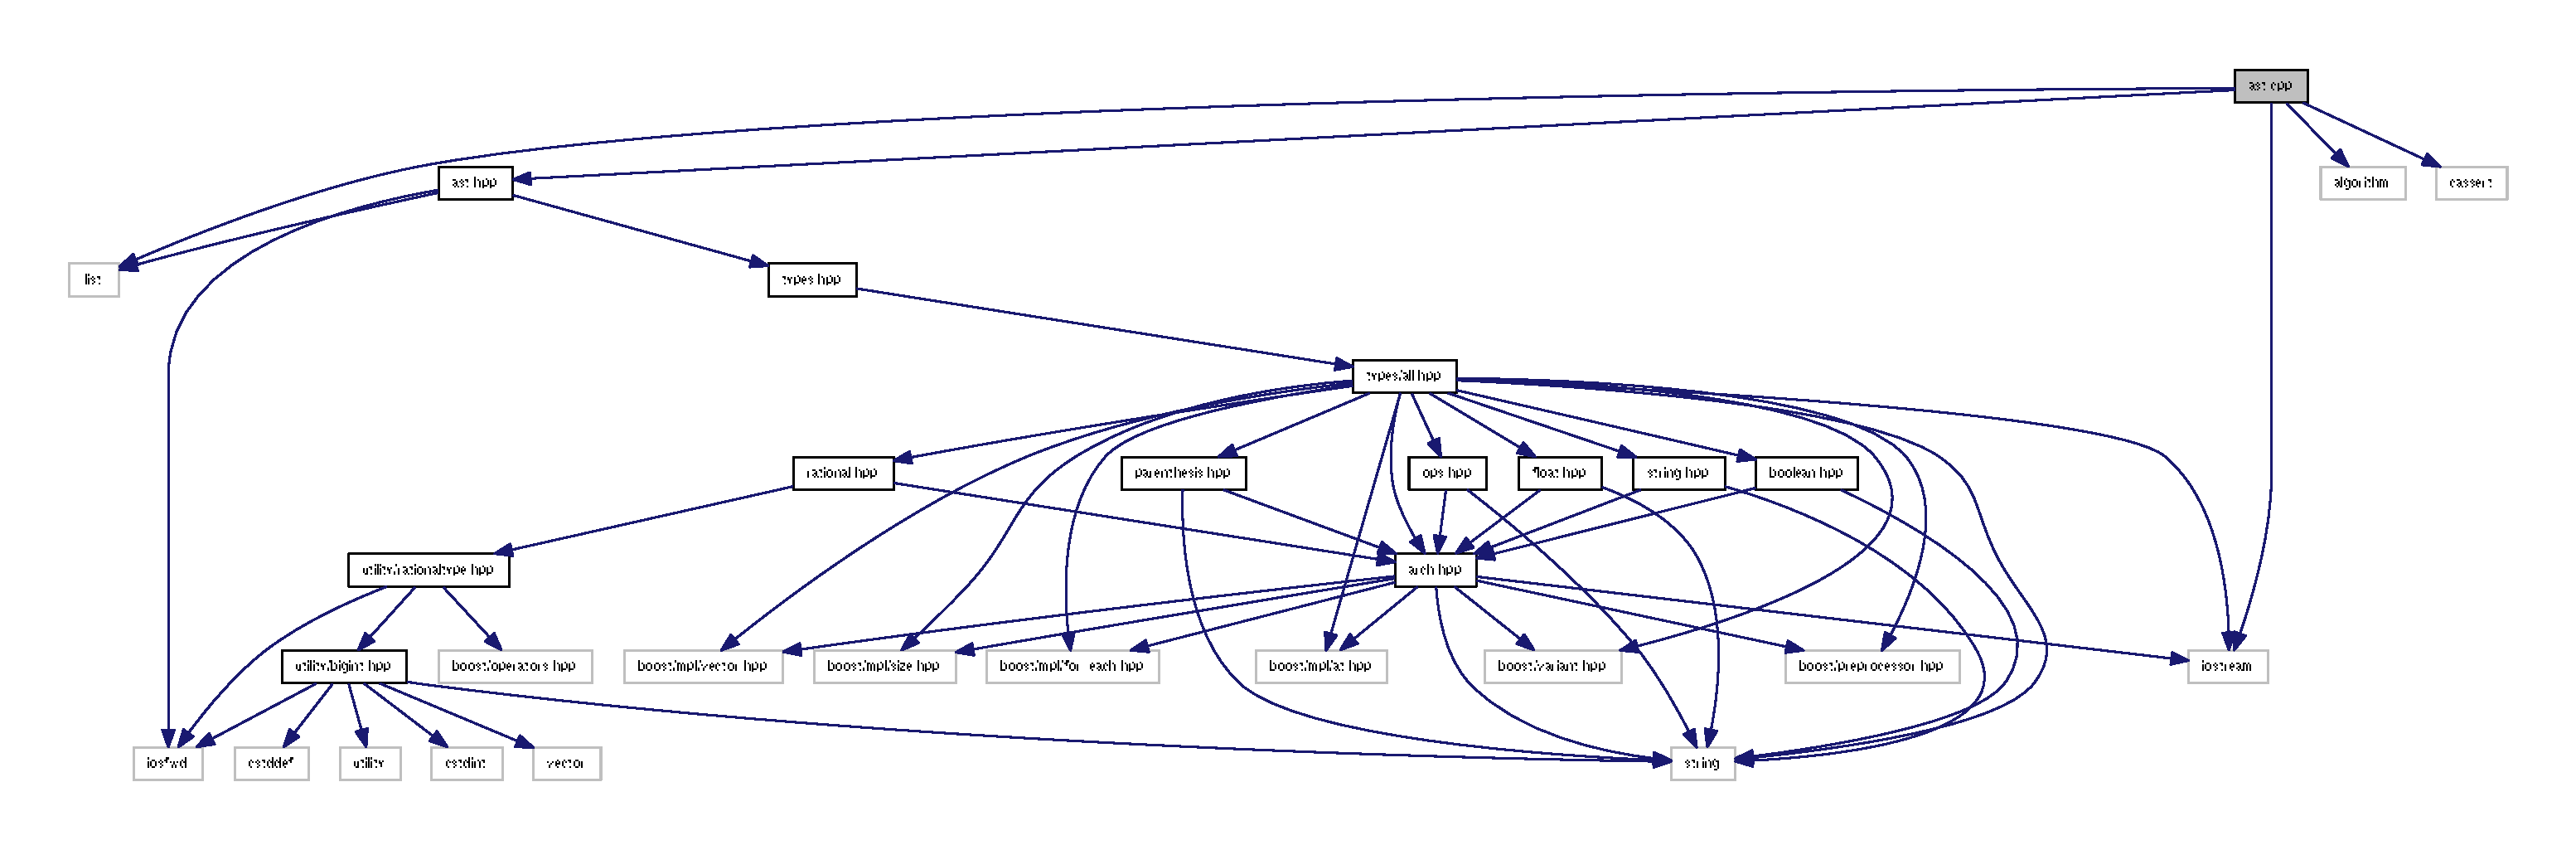
\includegraphics[width=350pt]{ast_8cpp__incl}
\end{center}
\end{figure}
\subsection*{Functions}
\begin{DoxyCompactItemize}
\item 
std\+::ostream \& \hyperlink{ast_8cpp_a92b9f335ac976192dab86fc6b59d357b}{operator$<$$<$} (std\+::ostream \&o, const \hyperlink{class_a_s_t}{A\+S\+T} \&\hyperlink{cli_8cpp_a3cc5b76560a60268fc81bfce22b51bf7}{ast})
\end{DoxyCompactItemize}


\subsection{Function Documentation}
\hypertarget{ast_8cpp_a92b9f335ac976192dab86fc6b59d357b}{}\index{ast.\+cpp@{ast.\+cpp}!operator$<$$<$@{operator$<$$<$}}
\index{operator$<$$<$@{operator$<$$<$}!ast.\+cpp@{ast.\+cpp}}
\subsubsection[{operator$<$$<$}]{\setlength{\rightskip}{0pt plus 5cm}std\+::ostream\& operator$<$$<$ (
\begin{DoxyParamCaption}
\item[{std\+::ostream \&}]{o, }
\item[{const {\bf A\+S\+T} \&}]{ast}
\end{DoxyParamCaption}
)}\label{ast_8cpp_a92b9f335ac976192dab86fc6b59d357b}


Definition at line 88 of file ast.\+cpp.


\hypertarget{ast_8hpp}{}\section{ast.\+hpp File Reference}
\label{ast_8hpp}\index{ast.\+hpp@{ast.\+hpp}}
{\ttfamily \#include $<$list$>$}\\*
{\ttfamily \#include $<$iosfwd$>$}\\*
{\ttfamily \#include \char`\"{}types.\+hpp\char`\"{}}\\*
Include dependency graph for ast.\+hpp\+:\nopagebreak
\begin{figure}[H]
\begin{center}
\leavevmode
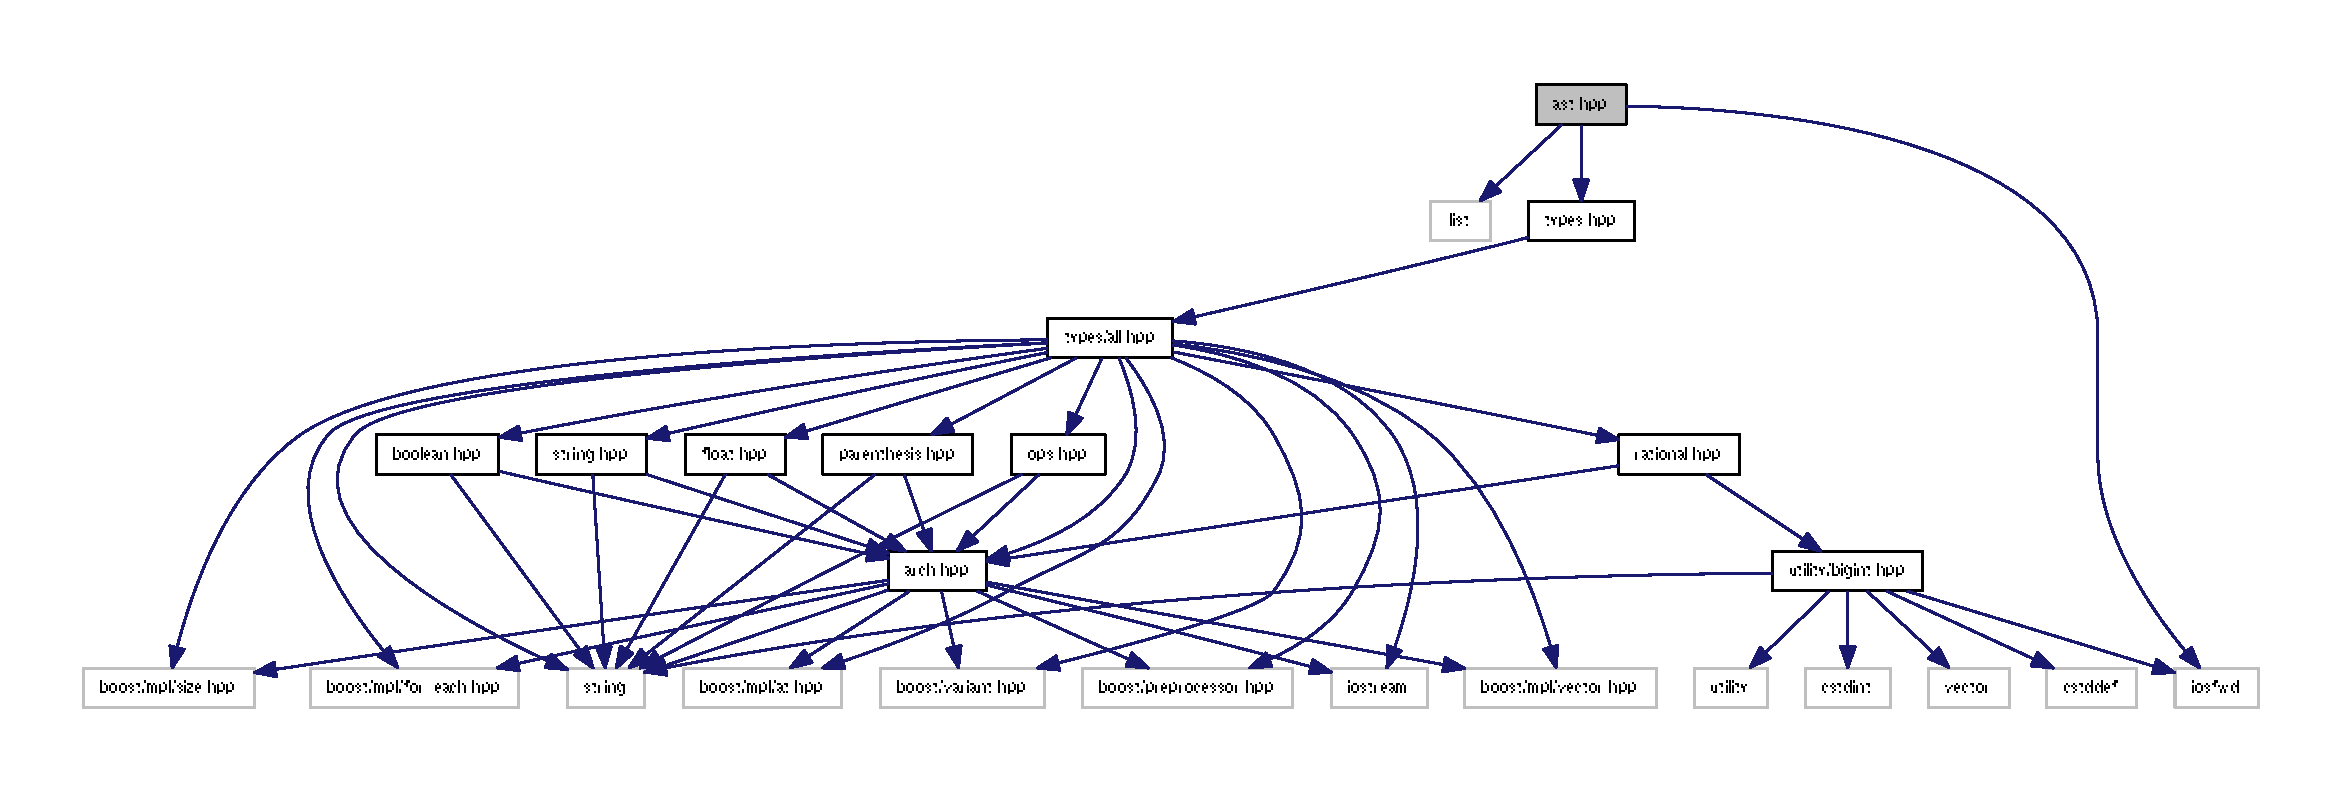
\includegraphics[width=350pt]{ast_8hpp__incl}
\end{center}
\end{figure}
This graph shows which files directly or indirectly include this file\+:\nopagebreak
\begin{figure}[H]
\begin{center}
\leavevmode
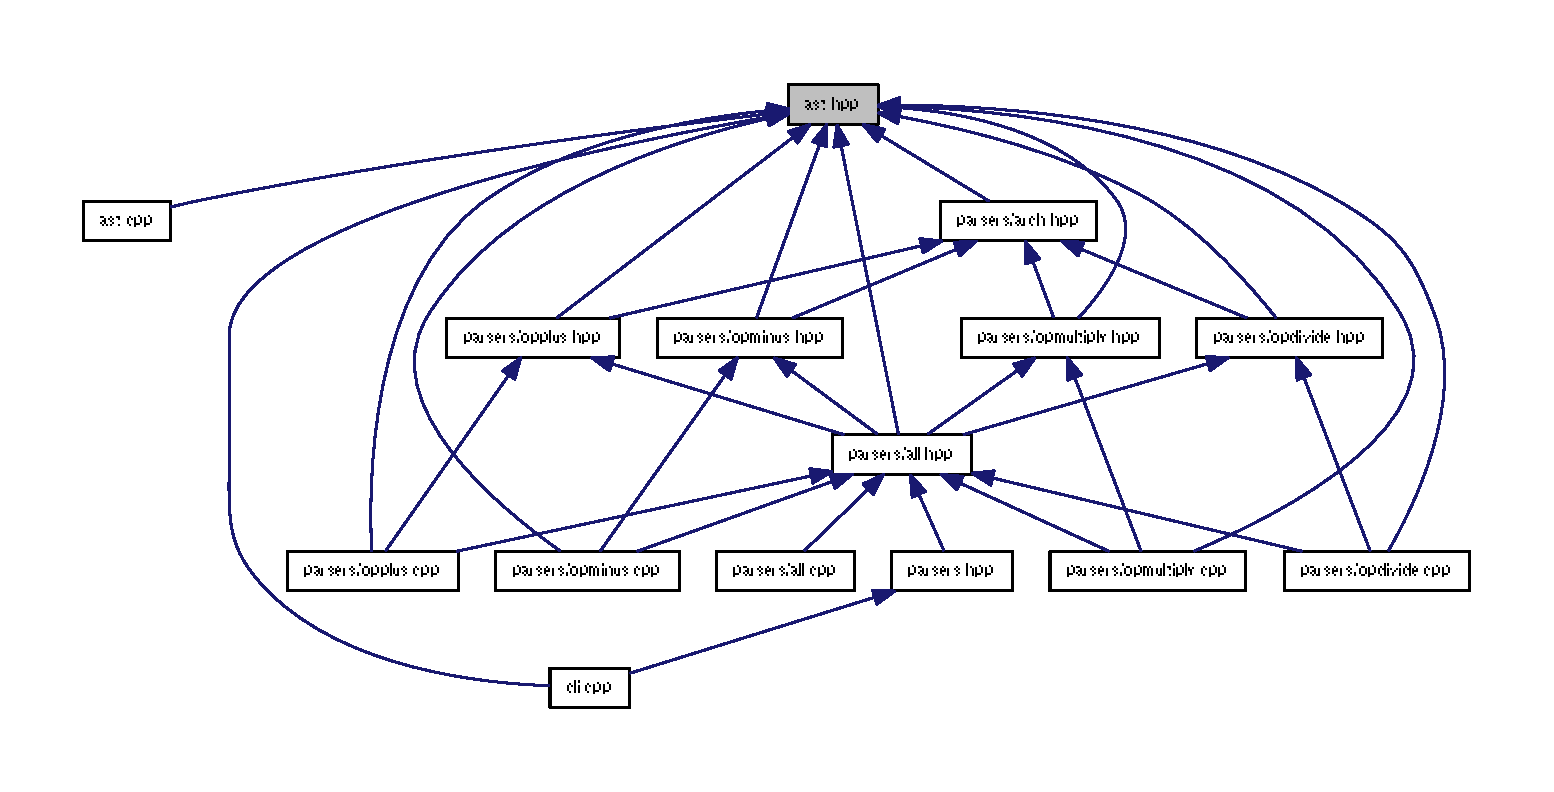
\includegraphics[width=123pt]{ast_8hpp__dep__incl}
\end{center}
\end{figure}
\subsection*{Classes}
\begin{DoxyCompactItemize}
\item 
struct \hyperlink{struct_a_s_t_node}{A\+S\+T\+Node}
\item 
class \hyperlink{class_a_s_t}{A\+S\+T}
\end{DoxyCompactItemize}
\subsection*{Enumerations}
\begin{DoxyCompactItemize}
\item 
enum \hyperlink{ast_8hpp_acac9cbaeea226ed297804c012dc12b16}{Node\+Type} \{ \hyperlink{ast_8hpp_acac9cbaeea226ed297804c012dc12b16a269c13c2affa9b7cff07a4aa1e9c5f2e}{Bracket}, 
\hyperlink{ast_8hpp_acac9cbaeea226ed297804c012dc12b16aebfbf7dc5cde0772efb1aa49712bd76b}{Simple}
 \}
\end{DoxyCompactItemize}


\subsection{Enumeration Type Documentation}
\hypertarget{ast_8hpp_acac9cbaeea226ed297804c012dc12b16}{}\index{ast.\+hpp@{ast.\+hpp}!Node\+Type@{Node\+Type}}
\index{Node\+Type@{Node\+Type}!ast.\+hpp@{ast.\+hpp}}
\subsubsection[{Node\+Type}]{\setlength{\rightskip}{0pt plus 5cm}enum {\bf Node\+Type}}\label{ast_8hpp_acac9cbaeea226ed297804c012dc12b16}
\begin{Desc}
\item[Enumerator]\par
\begin{description}
\index{Bracket@{Bracket}!ast.\+hpp@{ast.\+hpp}}\index{ast.\+hpp@{ast.\+hpp}!Bracket@{Bracket}}\item[{\em 
\hypertarget{ast_8hpp_acac9cbaeea226ed297804c012dc12b16a269c13c2affa9b7cff07a4aa1e9c5f2e}{}Bracket\label{ast_8hpp_acac9cbaeea226ed297804c012dc12b16a269c13c2affa9b7cff07a4aa1e9c5f2e}
}]\index{Simple@{Simple}!ast.\+hpp@{ast.\+hpp}}\index{ast.\+hpp@{ast.\+hpp}!Simple@{Simple}}\item[{\em 
\hypertarget{ast_8hpp_acac9cbaeea226ed297804c012dc12b16aebfbf7dc5cde0772efb1aa49712bd76b}{}Simple\label{ast_8hpp_acac9cbaeea226ed297804c012dc12b16aebfbf7dc5cde0772efb1aa49712bd76b}
}]\end{description}
\end{Desc}


Definition at line 7 of file ast.\+hpp.


\hypertarget{cli_8cpp}{}\section{cli.\+cpp File Reference}
\label{cli_8cpp}\index{cli.\+cpp@{cli.\+cpp}}
{\ttfamily \#include \char`\"{}preprocessor.\+hpp\char`\"{}}\\*
{\ttfamily \#include \char`\"{}tokenizer.\+hpp\char`\"{}}\\*
{\ttfamily \#include \char`\"{}ast.\+hpp\char`\"{}}\\*
{\ttfamily \#include \char`\"{}parsers.\+hpp\char`\"{}}\\*
{\ttfamily \#include \char`\"{}utility/debug.\+hpp\char`\"{}}\\*
{\ttfamily \#include $<$iostream$>$}\\*
{\ttfamily \#include $<$sstream$>$}\\*
{\ttfamily \#include $<$string$>$}\\*
{\ttfamily \#include $<$iomanip$>$}\\*
{\ttfamily \#include $<$stdexcept$>$}\\*
{\ttfamily \#include $<$algorithm$>$}\\*
{\ttfamily \#include $<$memory$>$}\\*
Include dependency graph for cli.\+cpp\+:
\nopagebreak
\begin{figure}[H]
\begin{center}
\leavevmode
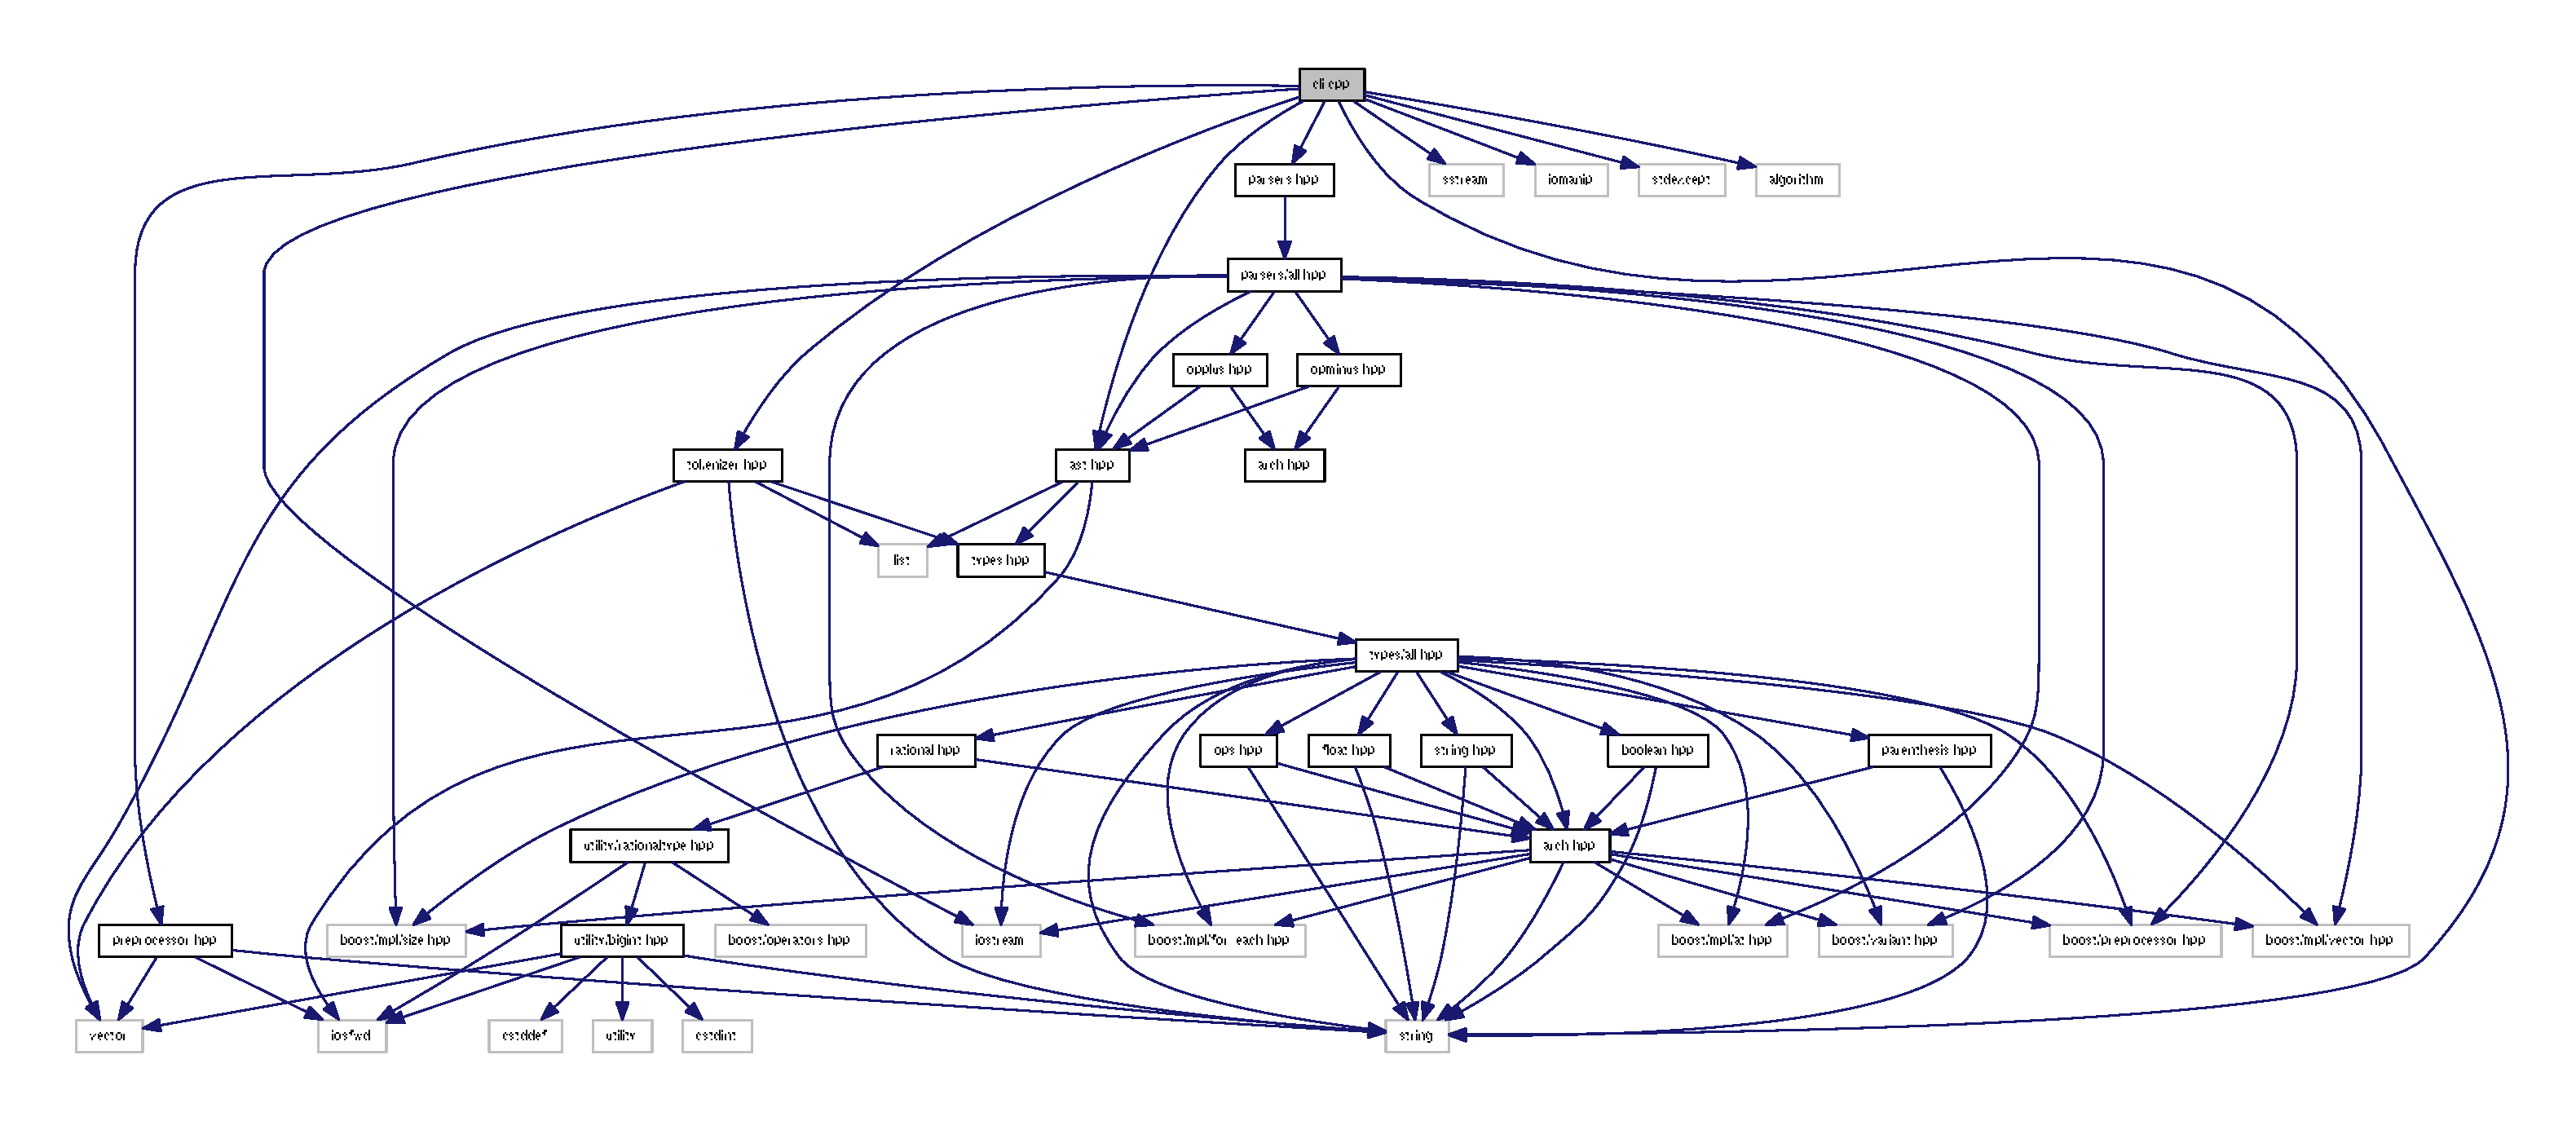
\includegraphics[width=350pt]{cli_8cpp__incl}
\end{center}
\end{figure}
\subsection*{Functions}
\begin{DoxyCompactItemize}
\item 
int \hyperlink{cli_8cpp_ae66f6b31b5ad750f1fe042a706a4e3d4}{main} ()
\end{DoxyCompactItemize}
\subsection*{Variables}
\begin{DoxyCompactItemize}
\item 
const std\+::string \hyperlink{cli_8cpp_a575d73a6aa36ed1a2a565301481cf822}{banner}
\item 
\hyperlink{class_scheme_unit}{Scheme\+Unit} \hyperlink{cli_8cpp_af9bc2698e658b28ab4b5abf475108e5c}{su}
\item 
\hyperlink{class_tokenizer}{Tokenizer} \hyperlink{cli_8cpp_a14a43a5183da558525c2fc14bac992b4}{to}
\item 
\hyperlink{class_a_s_t}{A\+S\+T} \hyperlink{cli_8cpp_a3cc5b76560a60268fc81bfce22b51bf7}{ast}
\item 
\hyperlink{class_parsers_helper}{Parsers\+Helper} \hyperlink{cli_8cpp_a4f3be538f49b526f4d43c11dae9e0cf9}{ph}
\item 
char $\ast$ \hyperlink{cli_8cpp_a1fe855c208bc17a51a4d34fefdb2d5b1}{buf}
\end{DoxyCompactItemize}


\subsection{Function Documentation}
\hypertarget{cli_8cpp_ae66f6b31b5ad750f1fe042a706a4e3d4}{}\index{cli.\+cpp@{cli.\+cpp}!main@{main}}
\index{main@{main}!cli.\+cpp@{cli.\+cpp}}
\subsubsection[{main}]{\setlength{\rightskip}{0pt plus 5cm}int main (
\begin{DoxyParamCaption}
{}
\end{DoxyParamCaption}
)}\label{cli_8cpp_ae66f6b31b5ad750f1fe042a706a4e3d4}


Definition at line 22 of file cli.\+cpp.



\subsection{Variable Documentation}
\hypertarget{cli_8cpp_a3cc5b76560a60268fc81bfce22b51bf7}{}\index{cli.\+cpp@{cli.\+cpp}!ast@{ast}}
\index{ast@{ast}!cli.\+cpp@{cli.\+cpp}}
\subsubsection[{ast}]{\setlength{\rightskip}{0pt plus 5cm}{\bf A\+S\+T} ast}\label{cli_8cpp_a3cc5b76560a60268fc81bfce22b51bf7}


Definition at line 19 of file cli.\+cpp.

\hypertarget{cli_8cpp_a575d73a6aa36ed1a2a565301481cf822}{}\index{cli.\+cpp@{cli.\+cpp}!banner@{banner}}
\index{banner@{banner}!cli.\+cpp@{cli.\+cpp}}
\subsubsection[{banner}]{\setlength{\rightskip}{0pt plus 5cm}const std\+::string banner}\label{cli_8cpp_a575d73a6aa36ed1a2a565301481cf822}
{\bfseries Initial value\+:}
\begin{DoxyCode}
= \textcolor{stringliteral}{"Welcome to htScheme! This version was compiled on "}+std::string(\_\_DATE\_\_)+ 
                            \textcolor{stringliteral}{" at "}+std::string(\_\_TIME\_\_)
\end{DoxyCode}


Definition at line 15 of file cli.\+cpp.

\hypertarget{cli_8cpp_a1fe855c208bc17a51a4d34fefdb2d5b1}{}\index{cli.\+cpp@{cli.\+cpp}!buf@{buf}}
\index{buf@{buf}!cli.\+cpp@{cli.\+cpp}}
\subsubsection[{buf}]{\setlength{\rightskip}{0pt plus 5cm}char$\ast$ buf}\label{cli_8cpp_a1fe855c208bc17a51a4d34fefdb2d5b1}


Definition at line 21 of file cli.\+cpp.

\hypertarget{cli_8cpp_a4f3be538f49b526f4d43c11dae9e0cf9}{}\index{cli.\+cpp@{cli.\+cpp}!ph@{ph}}
\index{ph@{ph}!cli.\+cpp@{cli.\+cpp}}
\subsubsection[{ph}]{\setlength{\rightskip}{0pt plus 5cm}{\bf Parsers\+Helper} ph}\label{cli_8cpp_a4f3be538f49b526f4d43c11dae9e0cf9}


Definition at line 20 of file cli.\+cpp.

\hypertarget{cli_8cpp_af9bc2698e658b28ab4b5abf475108e5c}{}\index{cli.\+cpp@{cli.\+cpp}!su@{su}}
\index{su@{su}!cli.\+cpp@{cli.\+cpp}}
\subsubsection[{su}]{\setlength{\rightskip}{0pt plus 5cm}{\bf Scheme\+Unit} su}\label{cli_8cpp_af9bc2698e658b28ab4b5abf475108e5c}


Definition at line 17 of file cli.\+cpp.

\hypertarget{cli_8cpp_a14a43a5183da558525c2fc14bac992b4}{}\index{cli.\+cpp@{cli.\+cpp}!to@{to}}
\index{to@{to}!cli.\+cpp@{cli.\+cpp}}
\subsubsection[{to}]{\setlength{\rightskip}{0pt plus 5cm}{\bf Tokenizer} to}\label{cli_8cpp_a14a43a5183da558525c2fc14bac992b4}


Definition at line 18 of file cli.\+cpp.


\hypertarget{dep_8d}{}\section{dep.\+d File Reference}
\label{dep_8d}\index{dep.\+d@{dep.\+d}}

\hypertarget{parsers_8hpp}{}\section{parsers.\+hpp File Reference}
\label{parsers_8hpp}\index{parsers.\+hpp@{parsers.\+hpp}}
{\ttfamily \#include \char`\"{}parsers/all.\+hpp\char`\"{}}\\*
Include dependency graph for parsers.\+hpp\+:
\nopagebreak
\begin{figure}[H]
\begin{center}
\leavevmode
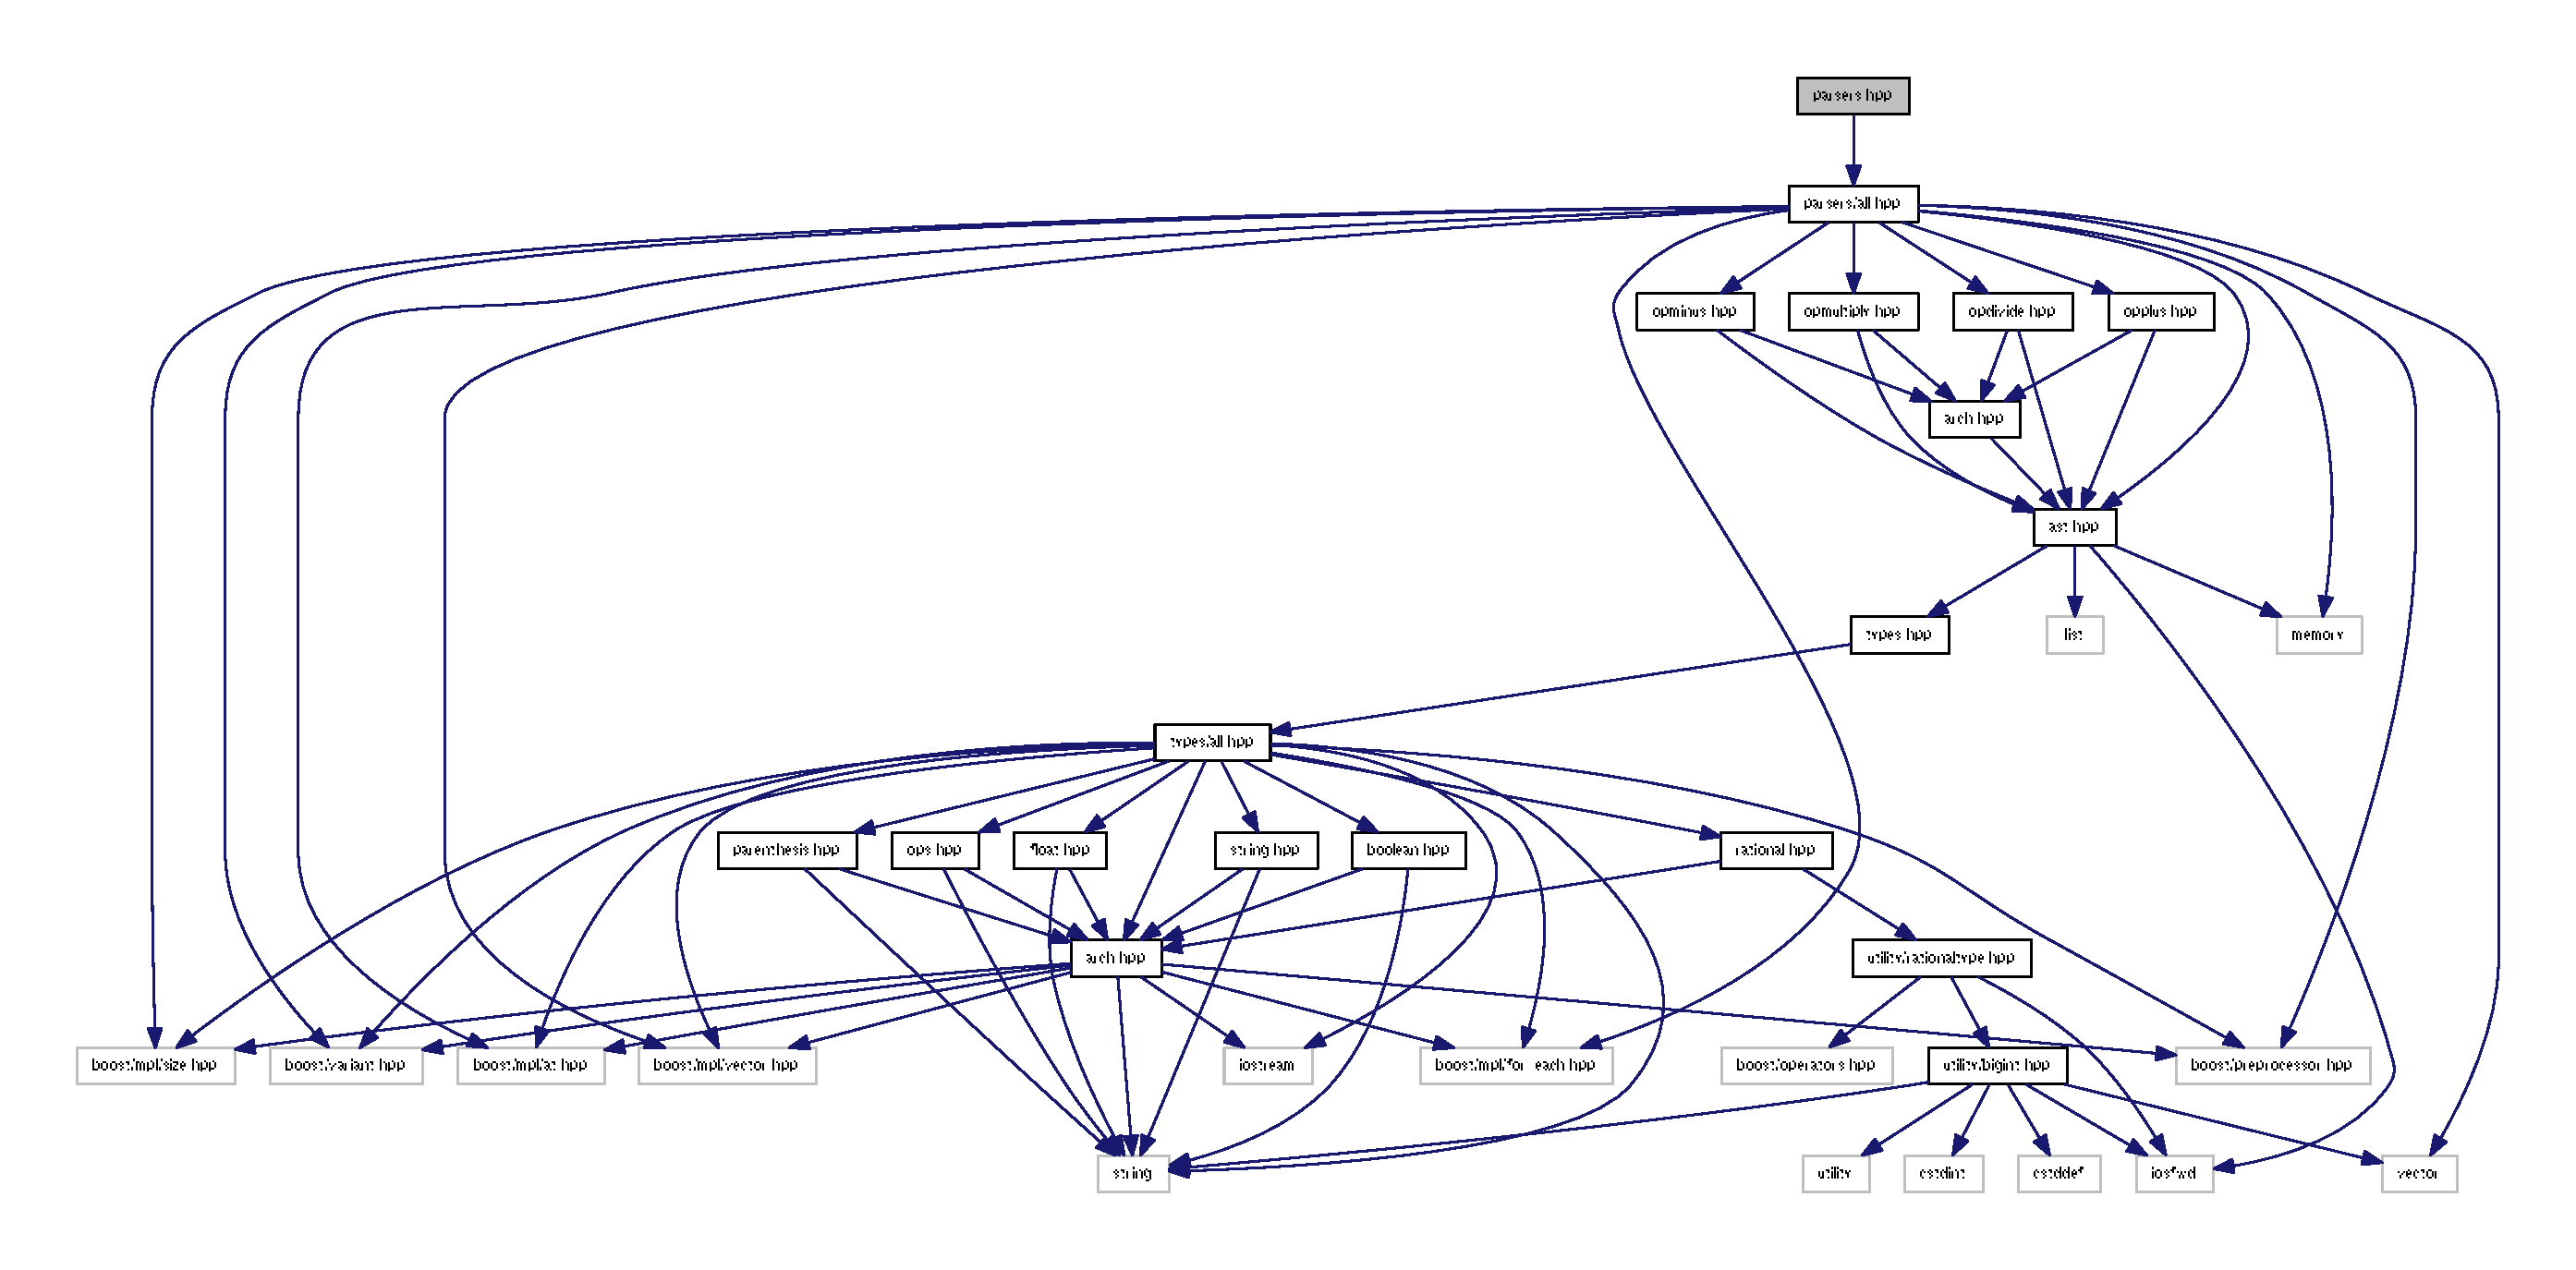
\includegraphics[width=350pt]{parsers_8hpp__incl}
\end{center}
\end{figure}
This graph shows which files directly or indirectly include this file\+:
\nopagebreak
\begin{figure}[H]
\begin{center}
\leavevmode
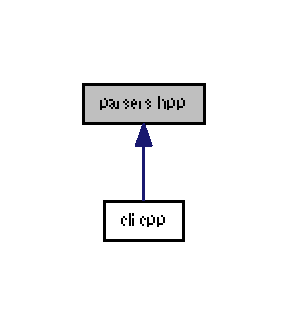
\includegraphics[width=138pt]{parsers_8hpp__dep__incl}
\end{center}
\end{figure}

\hypertarget{parsers_2all_8cpp}{}\section{parsers/all.cpp File Reference}
\label{parsers_2all_8cpp}\index{parsers/all.\+cpp@{parsers/all.\+cpp}}
{\ttfamily \#include \char`\"{}all.\+hpp\char`\"{}}\\*
{\ttfamily \#include \char`\"{}utility/debug.\+hpp\char`\"{}}\\*
{\ttfamily \#include $<$stdexcept$>$}\\*
{\ttfamily \#include $<$string$>$}\\*
{\ttfamily \#include $<$algorithm$>$}\\*
{\ttfamily \#include $<$memory$>$}\\*
Include dependency graph for all.\+cpp\+:
\nopagebreak
\begin{figure}[H]
\begin{center}
\leavevmode
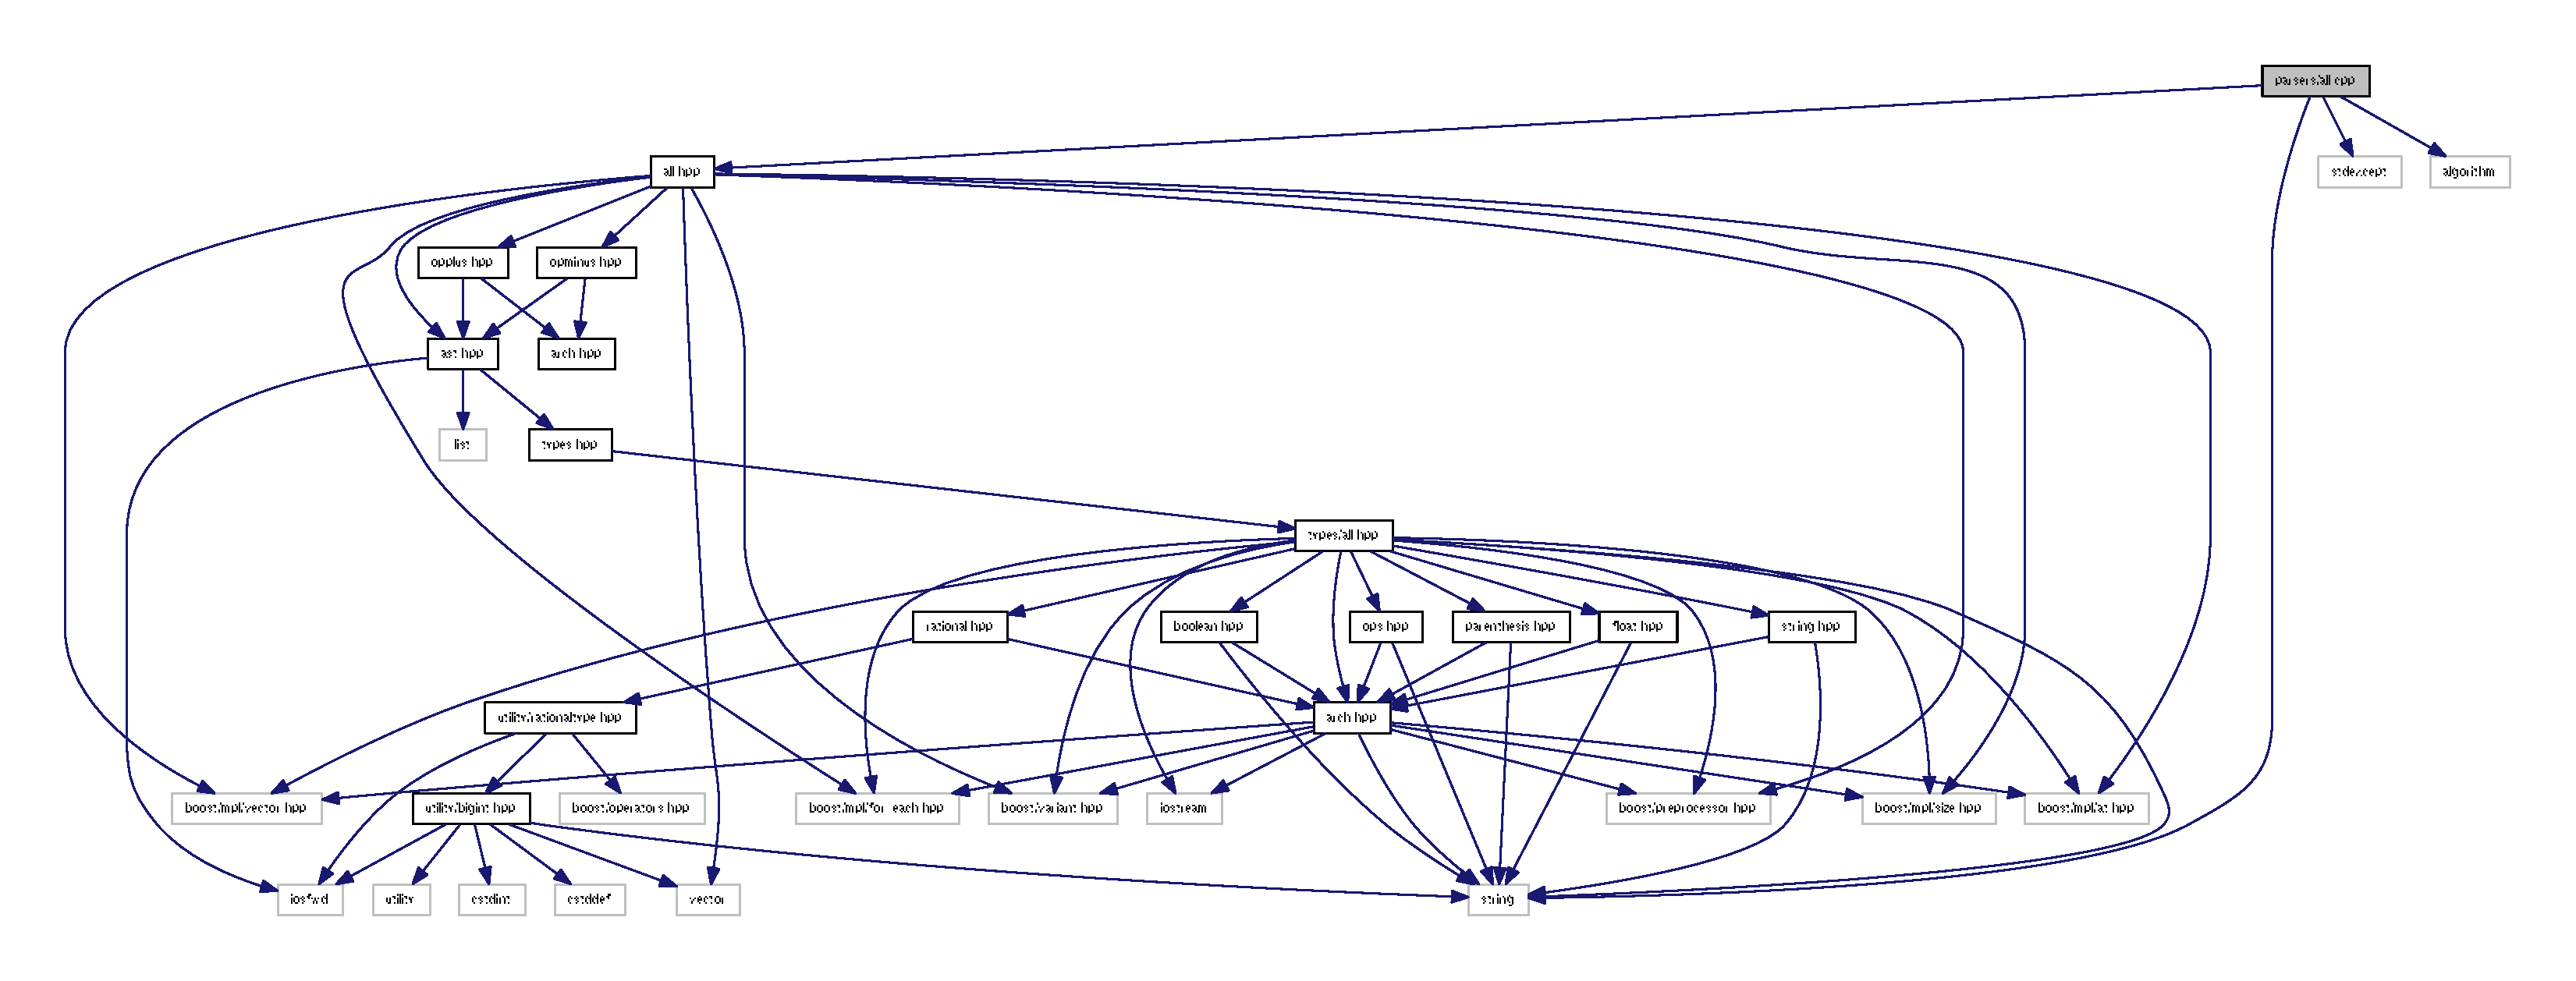
\includegraphics[width=350pt]{parsers_2all_8cpp__incl}
\end{center}
\end{figure}

\hypertarget{types_2all_8cpp}{}\section{types/all.cpp File Reference}
\label{types_2all_8cpp}\index{types/all.\+cpp@{types/all.\+cpp}}
{\ttfamily \#include \char`\"{}all.\+hpp\char`\"{}}\\*
{\ttfamily \#include $<$string$>$}\\*
Include dependency graph for all.\+cpp\+:
\nopagebreak
\begin{figure}[H]
\begin{center}
\leavevmode
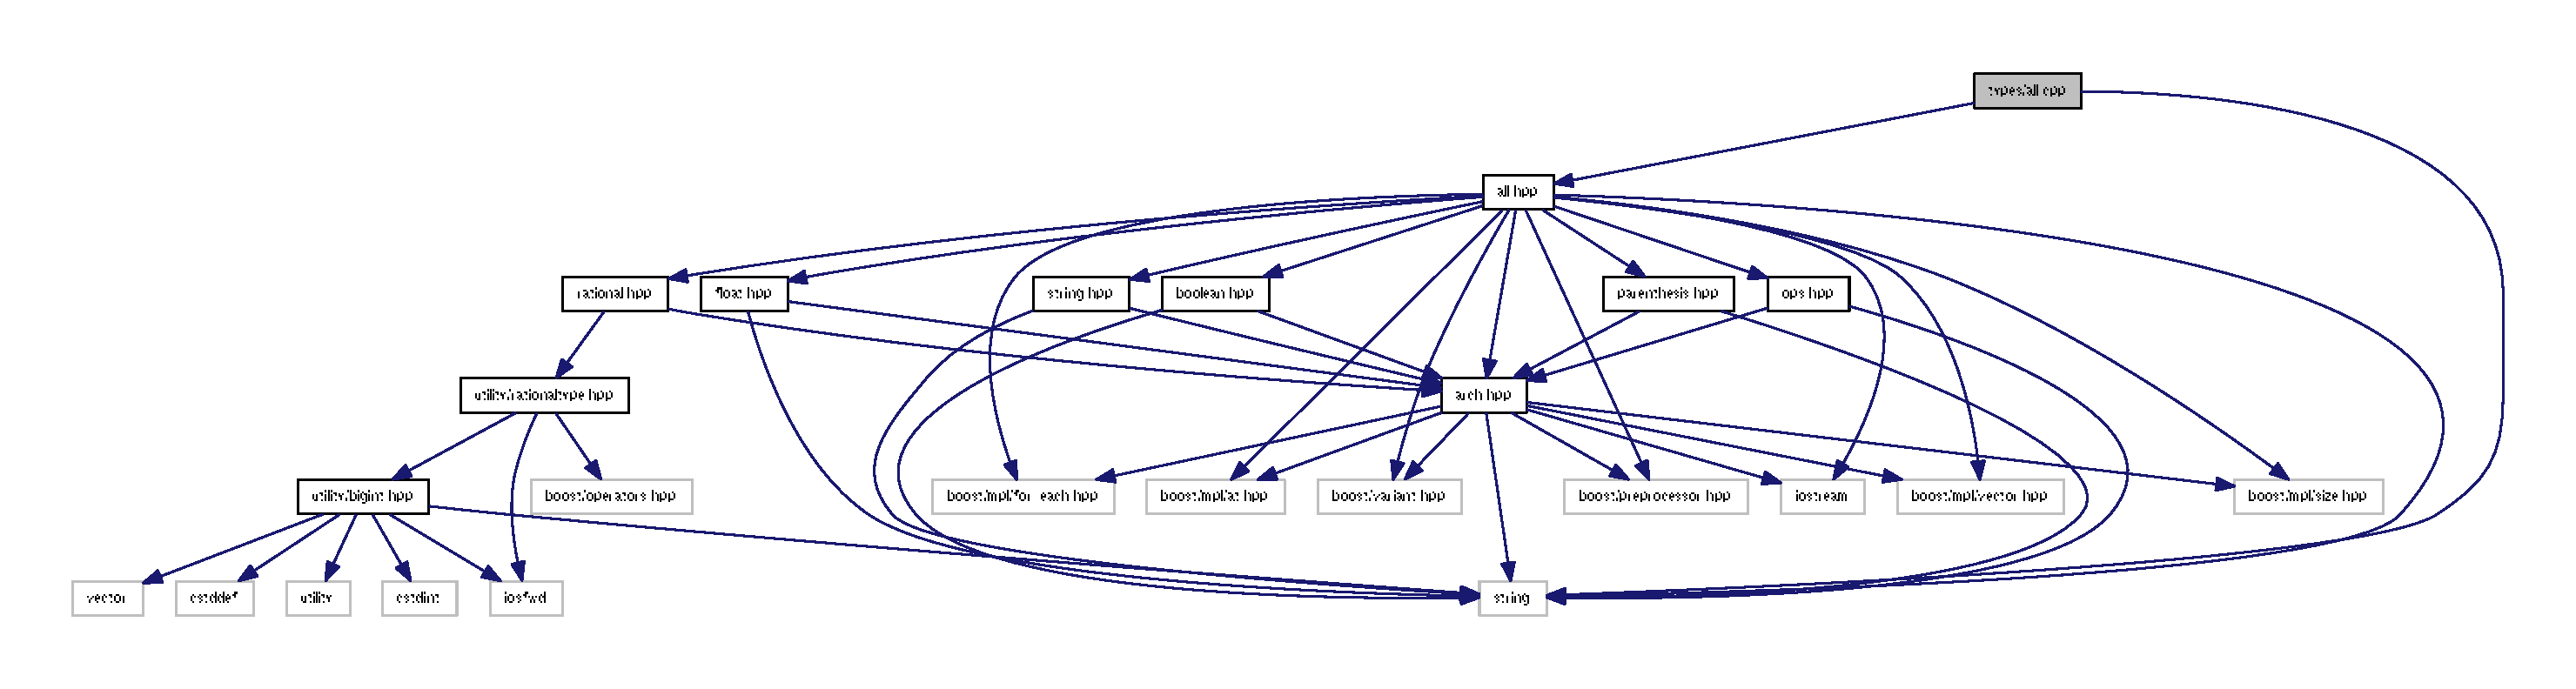
\includegraphics[width=350pt]{types_2all_8cpp__incl}
\end{center}
\end{figure}

\hypertarget{parsers_2all_8hpp}{}\section{parsers/all.hpp File Reference}
\label{parsers_2all_8hpp}\index{parsers/all.\+hpp@{parsers/all.\+hpp}}
{\ttfamily \#include $<$boost/mpl/size.\+hpp$>$}\\*
{\ttfamily \#include $<$boost/mpl/at.\+hpp$>$}\\*
{\ttfamily \#include $<$boost/mpl/vector.\+hpp$>$}\\*
{\ttfamily \#include $<$boost/mpl/for\+\_\+each.\+hpp$>$}\\*
{\ttfamily \#include $<$boost/variant.\+hpp$>$}\\*
{\ttfamily \#include $<$boost/preprocessor.\+hpp$>$}\\*
{\ttfamily \#include $<$vector$>$}\\*
{\ttfamily \#include \char`\"{}ast.\+hpp\char`\"{}}\\*
{\ttfamily \#include \char`\"{}opplus.\+hpp\char`\"{}}\\*
{\ttfamily \#include \char`\"{}opminus.\+hpp\char`\"{}}\\*
{\ttfamily \#include \char`\"{}opmultiply.\+hpp\char`\"{}}\\*
{\ttfamily \#include \char`\"{}opdivide.\+hpp\char`\"{}}\\*
{\ttfamily \#include $<$memory$>$}\\*
Include dependency graph for all.\+hpp\+:
\nopagebreak
\begin{figure}[H]
\begin{center}
\leavevmode
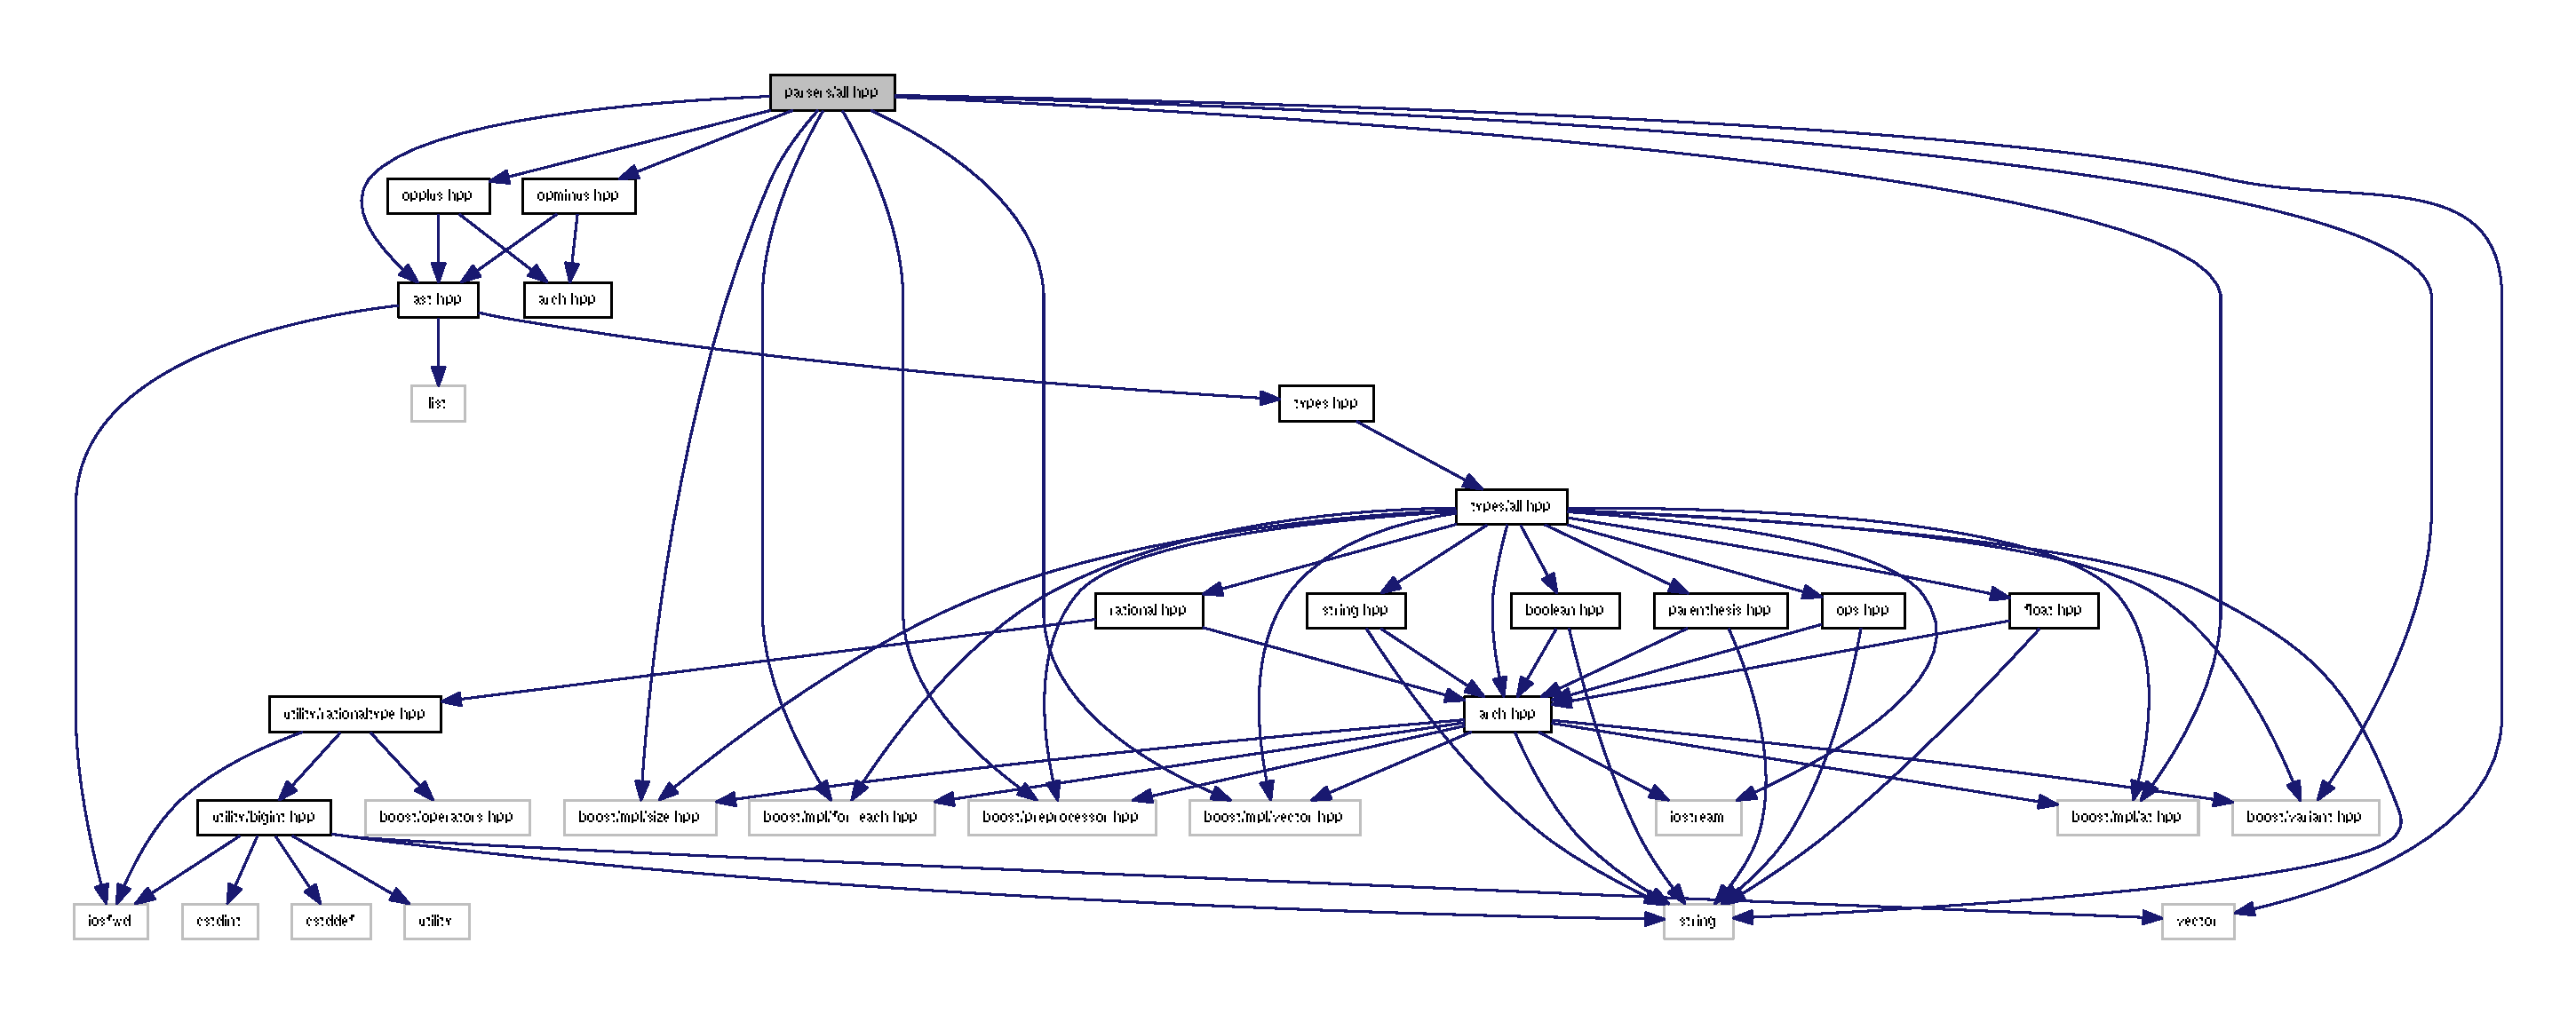
\includegraphics[width=350pt]{parsers_2all_8hpp__incl}
\end{center}
\end{figure}
This graph shows which files directly or indirectly include this file\+:\nopagebreak
\begin{figure}[H]
\begin{center}
\leavevmode
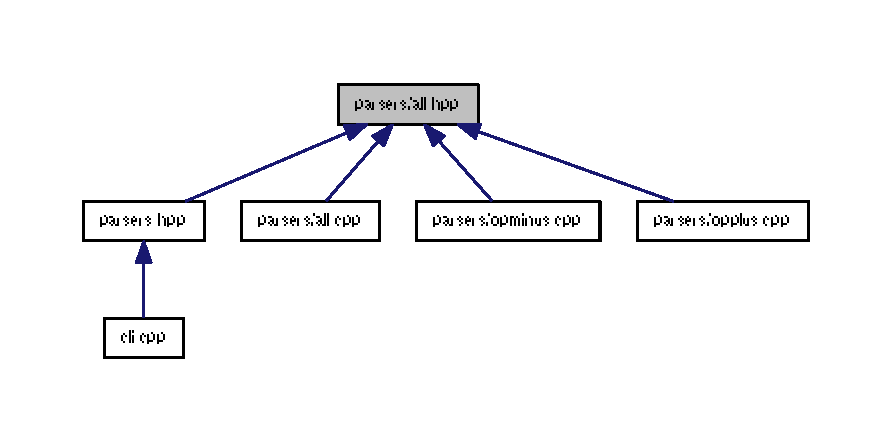
\includegraphics[width=350pt]{parsers_2all_8hpp__dep__incl}
\end{center}
\end{figure}
\subsection*{Classes}
\begin{DoxyCompactItemize}
\item 
class \hyperlink{class_parsers_helper}{Parsers\+Helper}
\end{DoxyCompactItemize}
\subsection*{Macros}
\begin{DoxyCompactItemize}
\item 
\#define \hyperlink{parsers_2all_8hpp_aad31e7dafe6570a7db6c133878e332e0}{A\+S\+T\+P\+A\+R\+S\+E\+R\+S\+\_\+\+T\+U\+P\+L\+E}~(\hyperlink{class_op_plus_a_s_t_parser}{Op\+Plus\+A\+S\+T\+Parser}, \hyperlink{class_op_minus_a_s_t_parser}{Op\+Minus\+A\+S\+T\+Parser}, \hyperlink{class_op_multiply_a_s_t_parser}{Op\+Multiply\+A\+S\+T\+Parser}, \hyperlink{class_op_divide_a_s_t_parser}{Op\+Divide\+A\+S\+T\+Parser})
\item 
\#define \hyperlink{parsers_2all_8hpp_a8a7554aba7ebc57553814b35aaaaa1a2}{A\+S\+T\+\_\+\+T\+U\+P\+L\+E\+S\+I\+Z\+E}~B\+O\+O\+S\+T\+\_\+\+P\+P\+\_\+\+T\+U\+P\+L\+E\+\_\+\+S\+I\+Z\+E(\hyperlink{parsers_2all_8hpp_aad31e7dafe6570a7db6c133878e332e0}{A\+S\+T\+P\+A\+R\+S\+E\+R\+S\+\_\+\+T\+U\+P\+L\+E})
\end{DoxyCompactItemize}
\subsection*{Typedefs}
\begin{DoxyCompactItemize}
\item 
typedef boost\+::mpl\+::vector$<$$>$ \hyperlink{parsers_2all_8hpp_ab9fa23d554df0c47fde3d3fa1dba7e02}{Parsers\+Type}
\item 
typedef boost\+::variant$<$ int, $>$ \hyperlink{parsers_2all_8hpp_abe36ed7c3b8a2eebe6d943c84fe72b9c}{Parser\+Type}
\end{DoxyCompactItemize}


\subsection{Macro Definition Documentation}
\hypertarget{parsers_2all_8hpp_a8a7554aba7ebc57553814b35aaaaa1a2}{}\index{parsers/all.\+hpp@{parsers/all.\+hpp}!A\+S\+T\+\_\+\+T\+U\+P\+L\+E\+S\+I\+Z\+E@{A\+S\+T\+\_\+\+T\+U\+P\+L\+E\+S\+I\+Z\+E}}
\index{A\+S\+T\+\_\+\+T\+U\+P\+L\+E\+S\+I\+Z\+E@{A\+S\+T\+\_\+\+T\+U\+P\+L\+E\+S\+I\+Z\+E}!parsers/all.\+hpp@{parsers/all.\+hpp}}
\subsubsection[{A\+S\+T\+\_\+\+T\+U\+P\+L\+E\+S\+I\+Z\+E}]{\setlength{\rightskip}{0pt plus 5cm}\#define A\+S\+T\+\_\+\+T\+U\+P\+L\+E\+S\+I\+Z\+E~B\+O\+O\+S\+T\+\_\+\+P\+P\+\_\+\+T\+U\+P\+L\+E\+\_\+\+S\+I\+Z\+E({\bf A\+S\+T\+P\+A\+R\+S\+E\+R\+S\+\_\+\+T\+U\+P\+L\+E})}\label{parsers_2all_8hpp_a8a7554aba7ebc57553814b35aaaaa1a2}


Definition at line 25 of file all.\+hpp.

\hypertarget{parsers_2all_8hpp_aad31e7dafe6570a7db6c133878e332e0}{}\index{parsers/all.\+hpp@{parsers/all.\+hpp}!A\+S\+T\+P\+A\+R\+S\+E\+R\+S\+\_\+\+T\+U\+P\+L\+E@{A\+S\+T\+P\+A\+R\+S\+E\+R\+S\+\_\+\+T\+U\+P\+L\+E}}
\index{A\+S\+T\+P\+A\+R\+S\+E\+R\+S\+\_\+\+T\+U\+P\+L\+E@{A\+S\+T\+P\+A\+R\+S\+E\+R\+S\+\_\+\+T\+U\+P\+L\+E}!parsers/all.\+hpp@{parsers/all.\+hpp}}
\subsubsection[{A\+S\+T\+P\+A\+R\+S\+E\+R\+S\+\_\+\+T\+U\+P\+L\+E}]{\setlength{\rightskip}{0pt plus 5cm}\#define A\+S\+T\+P\+A\+R\+S\+E\+R\+S\+\_\+\+T\+U\+P\+L\+E~({\bf Op\+Plus\+A\+S\+T\+Parser}, {\bf Op\+Minus\+A\+S\+T\+Parser}, {\bf Op\+Multiply\+A\+S\+T\+Parser}, {\bf Op\+Divide\+A\+S\+T\+Parser})}\label{parsers_2all_8hpp_aad31e7dafe6570a7db6c133878e332e0}


Definition at line 22 of file all.\+hpp.



\subsection{Typedef Documentation}
\hypertarget{parsers_2all_8hpp_ab9fa23d554df0c47fde3d3fa1dba7e02}{}\index{parsers/all.\+hpp@{parsers/all.\+hpp}!Parsers\+Type@{Parsers\+Type}}
\index{Parsers\+Type@{Parsers\+Type}!parsers/all.\+hpp@{parsers/all.\+hpp}}
\subsubsection[{Parsers\+Type}]{\setlength{\rightskip}{0pt plus 5cm}typedef boost\+::mpl\+::vector$<$$>$ {\bf Parsers\+Type}}\label{parsers_2all_8hpp_ab9fa23d554df0c47fde3d3fa1dba7e02}


Definition at line 29 of file all.\+hpp.

\hypertarget{parsers_2all_8hpp_abe36ed7c3b8a2eebe6d943c84fe72b9c}{}\index{parsers/all.\+hpp@{parsers/all.\+hpp}!Parser\+Type@{Parser\+Type}}
\index{Parser\+Type@{Parser\+Type}!parsers/all.\+hpp@{parsers/all.\+hpp}}
\subsubsection[{Parser\+Type}]{\setlength{\rightskip}{0pt plus 5cm}typedef boost\+::variant$<$int, $>$ {\bf Parser\+Type}}\label{parsers_2all_8hpp_abe36ed7c3b8a2eebe6d943c84fe72b9c}


Definition at line 32 of file all.\+hpp.


\hypertarget{types_2all_8hpp}{}\section{types/all.hpp File Reference}
\label{types_2all_8hpp}\index{types/all.\+hpp@{types/all.\+hpp}}
{\ttfamily \#include $<$iostream$>$}\\*
{\ttfamily \#include $<$string$>$}\\*
{\ttfamily \#include $<$boost/mpl/vector.\+hpp$>$}\\*
{\ttfamily \#include $<$boost/mpl/size.\+hpp$>$}\\*
{\ttfamily \#include $<$boost/mpl/for\+\_\+each.\+hpp$>$}\\*
{\ttfamily \#include $<$boost/mpl/at.\+hpp$>$}\\*
{\ttfamily \#include $<$boost/variant.\+hpp$>$}\\*
{\ttfamily \#include $<$boost/preprocessor.\+hpp$>$}\\*
{\ttfamily \#include \char`\"{}arch.\+hpp\char`\"{}}\\*
{\ttfamily \#include \char`\"{}rational.\+hpp\char`\"{}}\\*
{\ttfamily \#include \char`\"{}float.\+hpp\char`\"{}}\\*
{\ttfamily \#include \char`\"{}string.\+hpp\char`\"{}}\\*
{\ttfamily \#include \char`\"{}boolean.\+hpp\char`\"{}}\\*
{\ttfamily \#include \char`\"{}parenthesis.\+hpp\char`\"{}}\\*
{\ttfamily \#include \char`\"{}ops.\+hpp\char`\"{}}\\*
Include dependency graph for all.\+hpp\+:\nopagebreak
\begin{figure}[H]
\begin{center}
\leavevmode
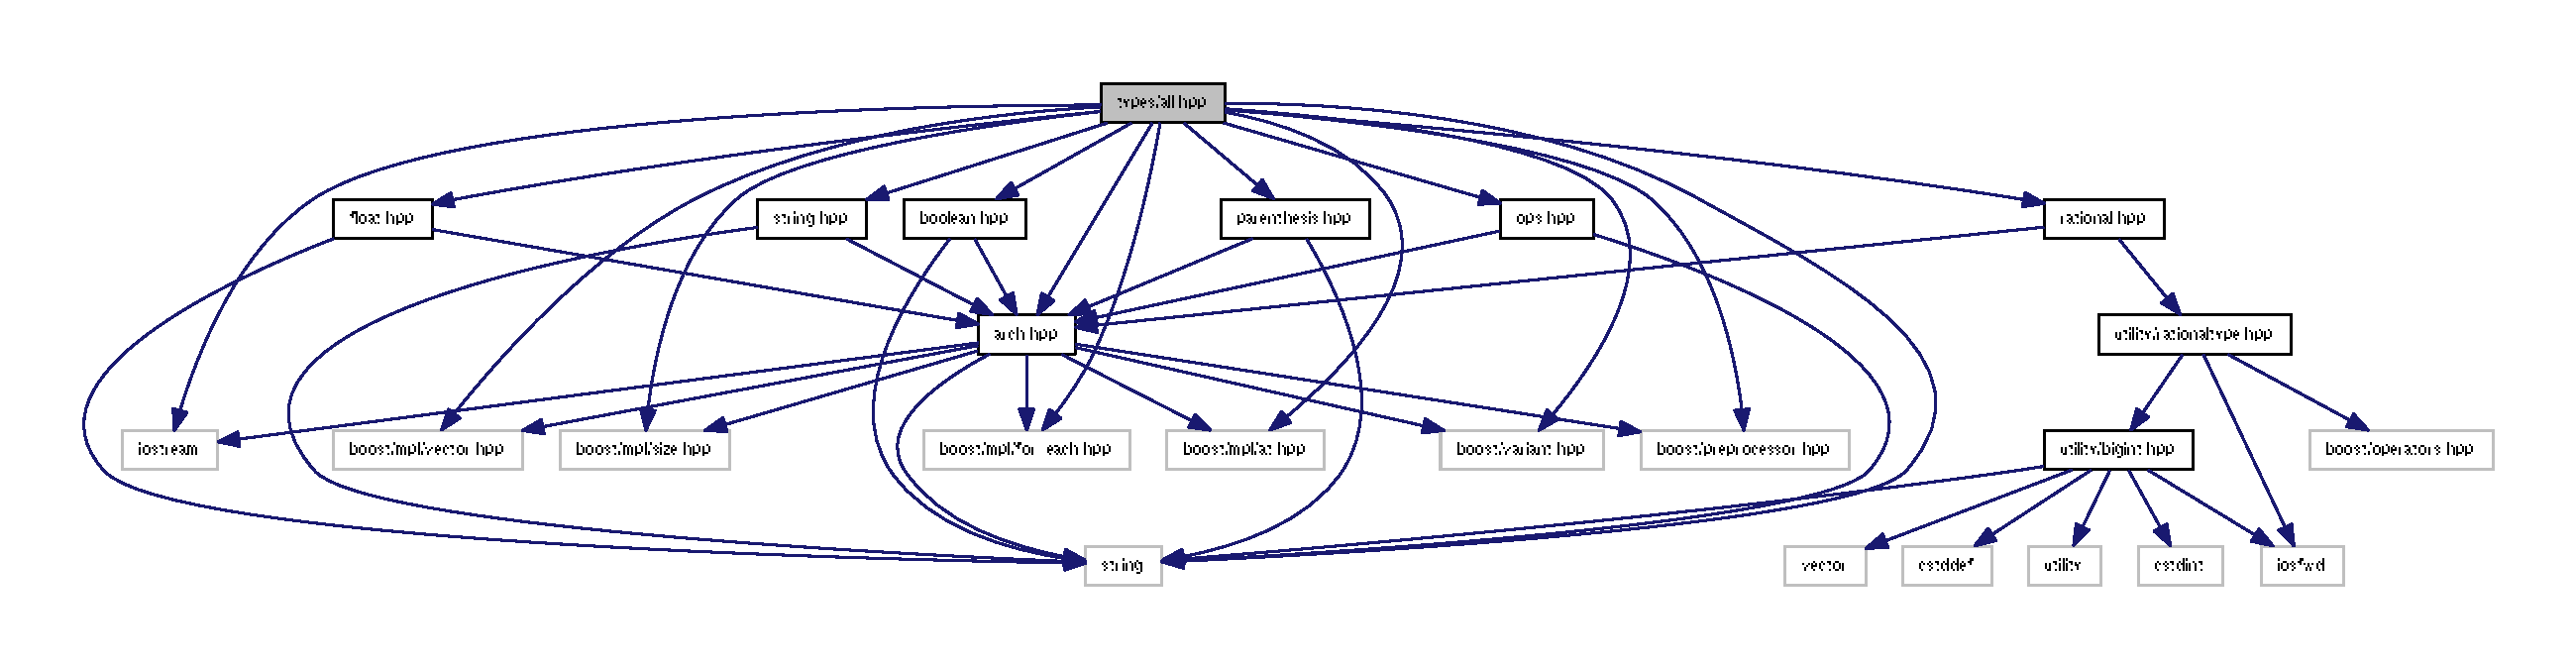
\includegraphics[width=350pt]{types_2all_8hpp__incl}
\end{center}
\end{figure}
This graph shows which files directly or indirectly include this file\+:
\nopagebreak
\begin{figure}[H]
\begin{center}
\leavevmode
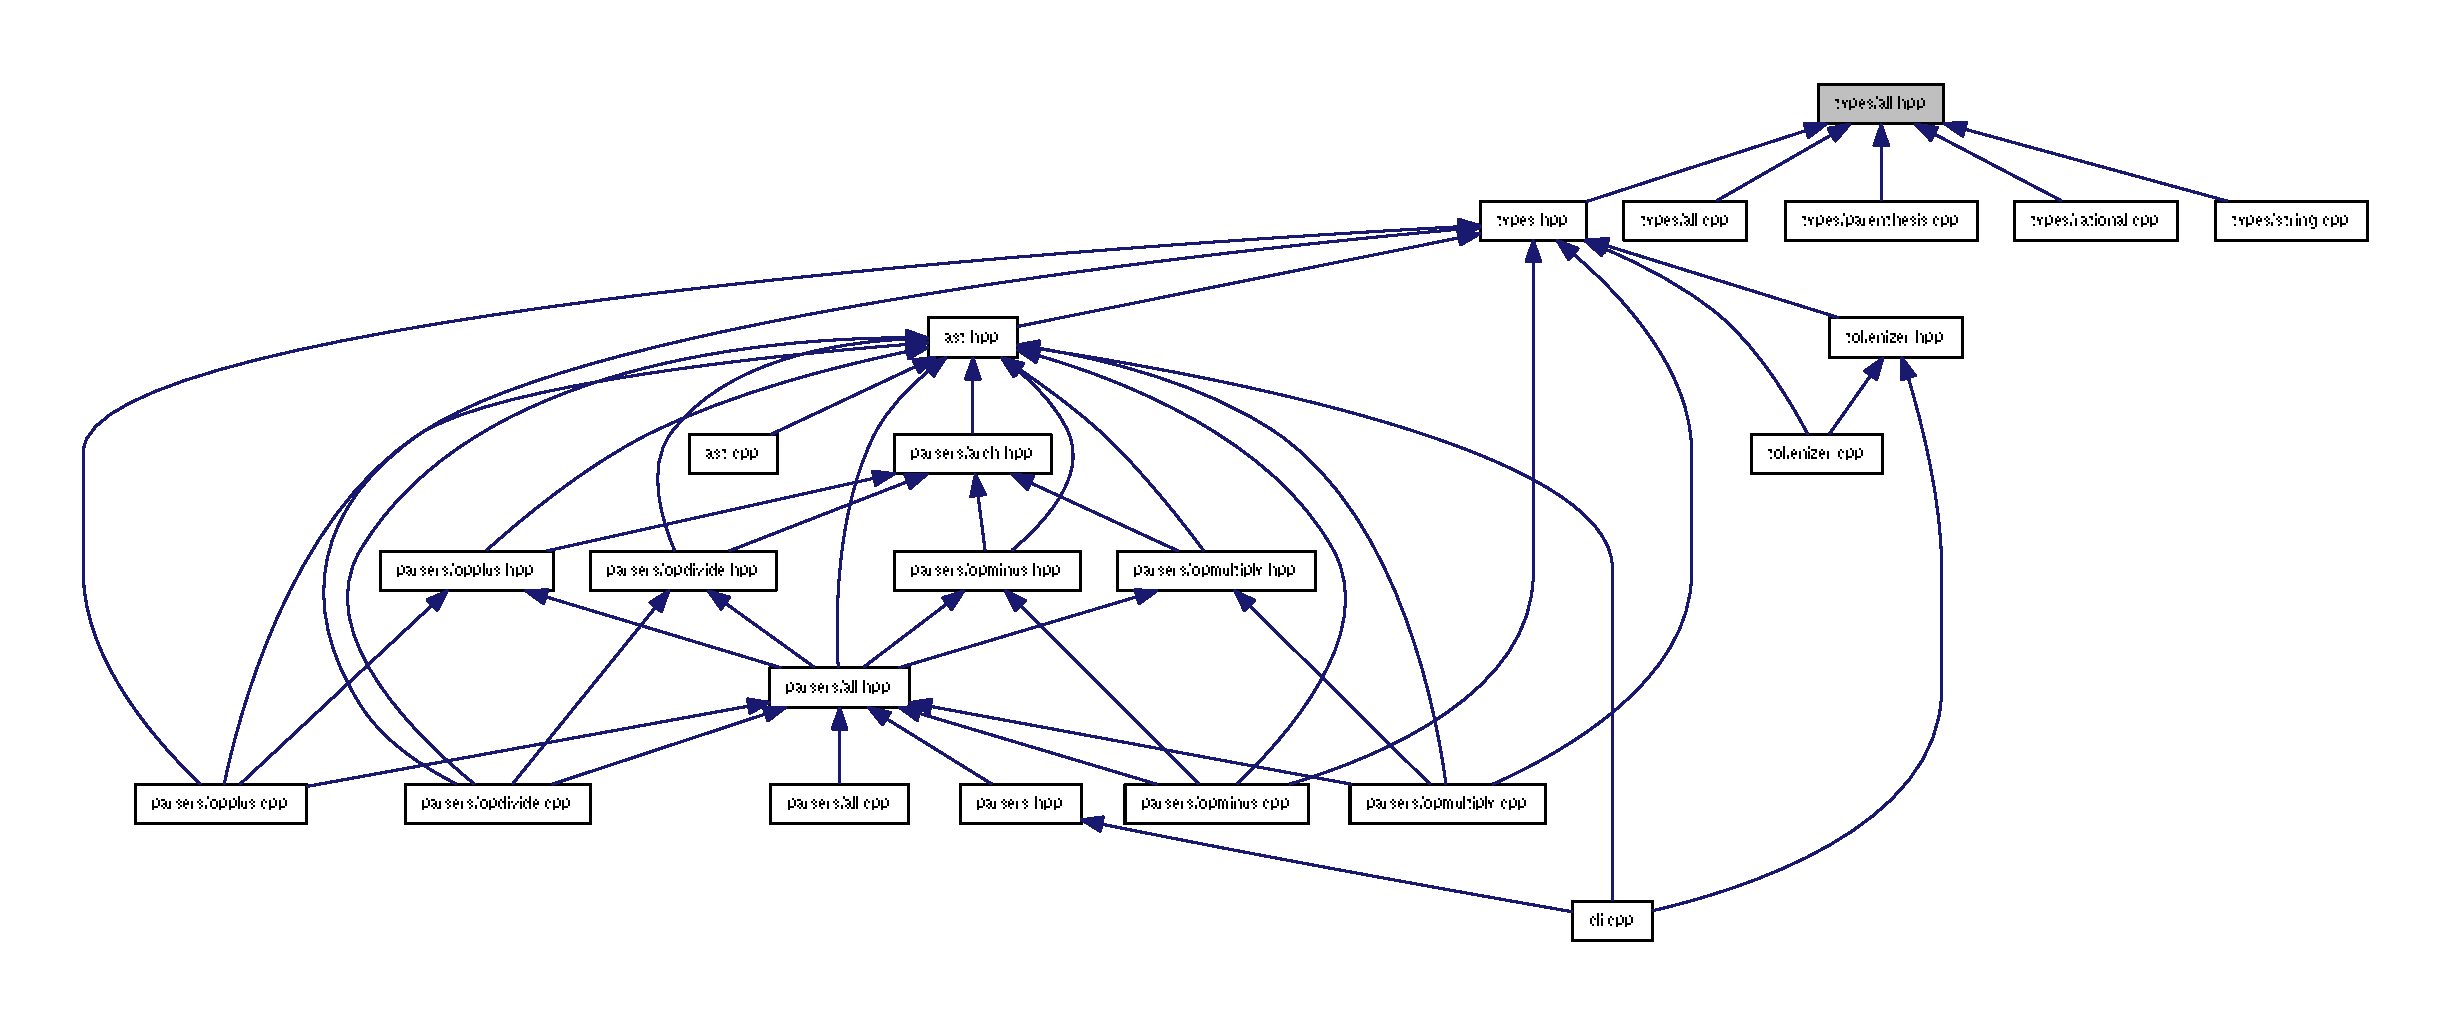
\includegraphics[width=350pt]{types_2all_8hpp__dep__incl}
\end{center}
\end{figure}
\subsection*{Classes}
\begin{DoxyCompactItemize}
\item 
struct \hyperlink{struct_token}{Token}
\item 
struct \hyperlink{struct_parser_visitor}{Parser\+Visitor}
\end{DoxyCompactItemize}
\subsection*{Macros}
\begin{DoxyCompactItemize}
\item 
\#define \hyperlink{types_2all_8hpp_aedfb3b5066f5f589249bfc4ab7b75e9b}{P\+A\+R\+S\+E\+R\+S\+\_\+\+T\+U\+P\+L\+E}
\item 
\#define \hyperlink{types_2all_8hpp_a1f22713d64ccb57c27c0a313ca1c6375}{P\+A\+R\+S\+E\+R\+S\+\_\+\+S\+I\+Z\+E}~B\+O\+O\+S\+T\+\_\+\+P\+P\+\_\+\+T\+U\+P\+L\+E\+\_\+\+S\+I\+Z\+E(\hyperlink{types_2all_8hpp_aedfb3b5066f5f589249bfc4ab7b75e9b}{P\+A\+R\+S\+E\+R\+S\+\_\+\+T\+U\+P\+L\+E})
\item 
\#define \hyperlink{types_2all_8hpp_ac172a4a9fd76e79c6cc98fbbf0faf9db}{B\+O\+O\+S\+T\+\_\+\+P\+P\+\_\+\+L\+O\+C\+A\+L\+\_\+\+L\+I\+M\+I\+T\+S}~(0,\hyperlink{types_2all_8hpp_a1f22713d64ccb57c27c0a313ca1c6375}{P\+A\+R\+S\+E\+R\+S\+\_\+\+S\+I\+Z\+E}-\/1)
\item 
\#define \hyperlink{types_2all_8hpp_a10331126934b04ed44afb0e1ed1cecf4}{B\+O\+O\+S\+T\+\_\+\+P\+P\+\_\+\+L\+O\+C\+A\+L\+\_\+\+M\+A\+C\+R\+O}(N)~boost\+::mpl\+::at\+\_\+c$<$\hyperlink{types_2all_8hpp_afcef35a3105632771c01dd22a5cb2bba}{parsers}, N$>$\+::type\+::\+Info\+Type,
\end{DoxyCompactItemize}
\subsection*{Typedefs}
\begin{DoxyCompactItemize}
\item 
typedef boost\+::mpl\+::vector$<$  $>$ \hyperlink{types_2all_8hpp_afcef35a3105632771c01dd22a5cb2bba}{parsers}
\item 
typedef boost\+::variant$<$ int $>$ \hyperlink{types_2all_8hpp_a58b4bafc5e94cba5e42b944a85b061db}{Info\+Types}
\end{DoxyCompactItemize}


\subsection{Macro Definition Documentation}
\hypertarget{types_2all_8hpp_ac172a4a9fd76e79c6cc98fbbf0faf9db}{}\index{types/all.\+hpp@{types/all.\+hpp}!B\+O\+O\+S\+T\+\_\+\+P\+P\+\_\+\+L\+O\+C\+A\+L\+\_\+\+L\+I\+M\+I\+T\+S@{B\+O\+O\+S\+T\+\_\+\+P\+P\+\_\+\+L\+O\+C\+A\+L\+\_\+\+L\+I\+M\+I\+T\+S}}
\index{B\+O\+O\+S\+T\+\_\+\+P\+P\+\_\+\+L\+O\+C\+A\+L\+\_\+\+L\+I\+M\+I\+T\+S@{B\+O\+O\+S\+T\+\_\+\+P\+P\+\_\+\+L\+O\+C\+A\+L\+\_\+\+L\+I\+M\+I\+T\+S}!types/all.\+hpp@{types/all.\+hpp}}
\subsubsection[{B\+O\+O\+S\+T\+\_\+\+P\+P\+\_\+\+L\+O\+C\+A\+L\+\_\+\+L\+I\+M\+I\+T\+S}]{\setlength{\rightskip}{0pt plus 5cm}\#define B\+O\+O\+S\+T\+\_\+\+P\+P\+\_\+\+L\+O\+C\+A\+L\+\_\+\+L\+I\+M\+I\+T\+S~(0,{\bf P\+A\+R\+S\+E\+R\+S\+\_\+\+S\+I\+Z\+E}-\/1)}\label{types_2all_8hpp_ac172a4a9fd76e79c6cc98fbbf0faf9db}


Definition at line 32 of file all.\+hpp.

\hypertarget{types_2all_8hpp_a10331126934b04ed44afb0e1ed1cecf4}{}\index{types/all.\+hpp@{types/all.\+hpp}!B\+O\+O\+S\+T\+\_\+\+P\+P\+\_\+\+L\+O\+C\+A\+L\+\_\+\+M\+A\+C\+R\+O@{B\+O\+O\+S\+T\+\_\+\+P\+P\+\_\+\+L\+O\+C\+A\+L\+\_\+\+M\+A\+C\+R\+O}}
\index{B\+O\+O\+S\+T\+\_\+\+P\+P\+\_\+\+L\+O\+C\+A\+L\+\_\+\+M\+A\+C\+R\+O@{B\+O\+O\+S\+T\+\_\+\+P\+P\+\_\+\+L\+O\+C\+A\+L\+\_\+\+M\+A\+C\+R\+O}!types/all.\+hpp@{types/all.\+hpp}}
\subsubsection[{B\+O\+O\+S\+T\+\_\+\+P\+P\+\_\+\+L\+O\+C\+A\+L\+\_\+\+M\+A\+C\+R\+O}]{\setlength{\rightskip}{0pt plus 5cm}\#define B\+O\+O\+S\+T\+\_\+\+P\+P\+\_\+\+L\+O\+C\+A\+L\+\_\+\+M\+A\+C\+R\+O(
\begin{DoxyParamCaption}
\item[{}]{N}
\end{DoxyParamCaption}
)~boost\+::mpl\+::at\+\_\+c$<${\bf parsers}, N$>$\+::type\+::\+Info\+Type,}\label{types_2all_8hpp_a10331126934b04ed44afb0e1ed1cecf4}


Definition at line 33 of file all.\+hpp.

\hypertarget{types_2all_8hpp_a1f22713d64ccb57c27c0a313ca1c6375}{}\index{types/all.\+hpp@{types/all.\+hpp}!P\+A\+R\+S\+E\+R\+S\+\_\+\+S\+I\+Z\+E@{P\+A\+R\+S\+E\+R\+S\+\_\+\+S\+I\+Z\+E}}
\index{P\+A\+R\+S\+E\+R\+S\+\_\+\+S\+I\+Z\+E@{P\+A\+R\+S\+E\+R\+S\+\_\+\+S\+I\+Z\+E}!types/all.\+hpp@{types/all.\+hpp}}
\subsubsection[{P\+A\+R\+S\+E\+R\+S\+\_\+\+S\+I\+Z\+E}]{\setlength{\rightskip}{0pt plus 5cm}\#define P\+A\+R\+S\+E\+R\+S\+\_\+\+S\+I\+Z\+E~B\+O\+O\+S\+T\+\_\+\+P\+P\+\_\+\+T\+U\+P\+L\+E\+\_\+\+S\+I\+Z\+E({\bf P\+A\+R\+S\+E\+R\+S\+\_\+\+T\+U\+P\+L\+E})}\label{types_2all_8hpp_a1f22713d64ccb57c27c0a313ca1c6375}


Definition at line 26 of file all.\+hpp.

\hypertarget{types_2all_8hpp_aedfb3b5066f5f589249bfc4ab7b75e9b}{}\index{types/all.\+hpp@{types/all.\+hpp}!P\+A\+R\+S\+E\+R\+S\+\_\+\+T\+U\+P\+L\+E@{P\+A\+R\+S\+E\+R\+S\+\_\+\+T\+U\+P\+L\+E}}
\index{P\+A\+R\+S\+E\+R\+S\+\_\+\+T\+U\+P\+L\+E@{P\+A\+R\+S\+E\+R\+S\+\_\+\+T\+U\+P\+L\+E}!types/all.\+hpp@{types/all.\+hpp}}
\subsubsection[{P\+A\+R\+S\+E\+R\+S\+\_\+\+T\+U\+P\+L\+E}]{\setlength{\rightskip}{0pt plus 5cm}\#define P\+A\+R\+S\+E\+R\+S\+\_\+\+T\+U\+P\+L\+E}\label{types_2all_8hpp_aedfb3b5066f5f589249bfc4ab7b75e9b}
{\bfseries Value\+:}
\begin{DoxyCode}
(BooleanParser, RationalParser, \(\backslash\)
                        OpPlusParser, OpMinusParser, OpMultiplyParser, OpDivideParser , FloatParser ,\(\backslash\)
                        StringParser , LeftParenthesisParser, RightParenthesisParser)
\end{DoxyCode}


Definition at line 21 of file all.\+hpp.



\subsection{Typedef Documentation}
\hypertarget{types_2all_8hpp_a58b4bafc5e94cba5e42b944a85b061db}{}\index{types/all.\+hpp@{types/all.\+hpp}!Info\+Types@{Info\+Types}}
\index{Info\+Types@{Info\+Types}!types/all.\+hpp@{types/all.\+hpp}}
\subsubsection[{Info\+Types}]{\setlength{\rightskip}{0pt plus 5cm}typedef boost\+::variant$<$int $>$ {\bf Info\+Types}}\label{types_2all_8hpp_a58b4bafc5e94cba5e42b944a85b061db}


Definition at line 40 of file all.\+hpp.

\hypertarget{types_2all_8hpp_afcef35a3105632771c01dd22a5cb2bba}{}\index{types/all.\+hpp@{types/all.\+hpp}!parsers@{parsers}}
\index{parsers@{parsers}!types/all.\+hpp@{types/all.\+hpp}}
\subsubsection[{parsers}]{\setlength{\rightskip}{0pt plus 5cm}typedef boost\+::mpl\+::vector$<$ $>$ {\bf parsers}}\label{types_2all_8hpp_afcef35a3105632771c01dd22a5cb2bba}


Definition at line 30 of file all.\+hpp.


\hypertarget{parsers_2arch_8hpp}{}\section{parsers/arch.hpp File Reference}
\label{parsers_2arch_8hpp}\index{parsers/arch.\+hpp@{parsers/arch.\+hpp}}
This graph shows which files directly or indirectly include this file\+:
\nopagebreak
\begin{figure}[H]
\begin{center}
\leavevmode
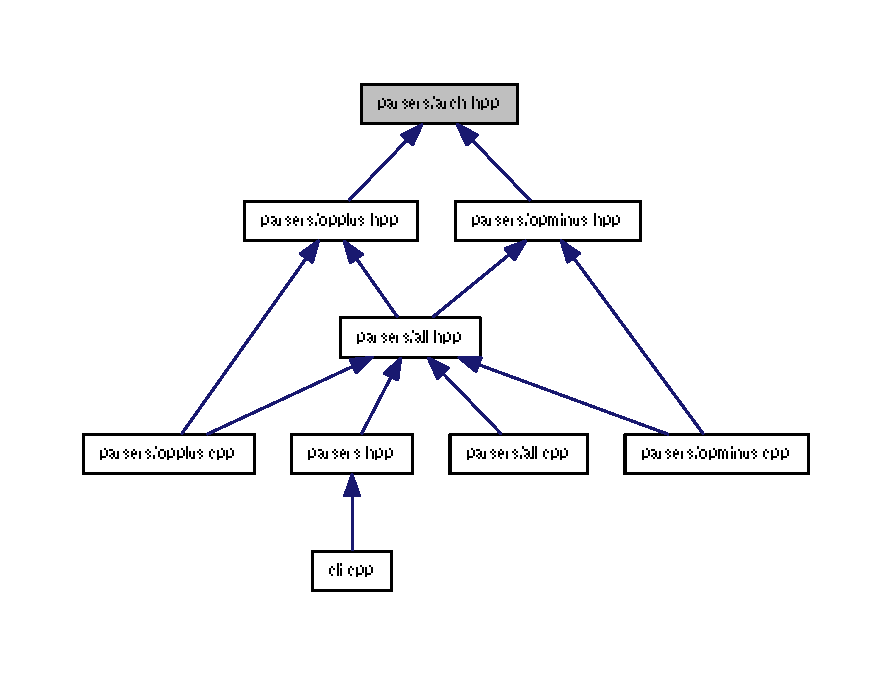
\includegraphics[width=350pt]{parsers_2arch_8hpp__dep__incl}
\end{center}
\end{figure}

\hypertarget{types_2arch_8hpp}{}\section{types/arch.hpp File Reference}
\label{types_2arch_8hpp}\index{types/arch.\+hpp@{types/arch.\+hpp}}
{\ttfamily \#include $<$iostream$>$}\\*
{\ttfamily \#include $<$string$>$}\\*
{\ttfamily \#include $<$boost/mpl/vector.\+hpp$>$}\\*
{\ttfamily \#include $<$boost/mpl/size.\+hpp$>$}\\*
{\ttfamily \#include $<$boost/mpl/for\+\_\+each.\+hpp$>$}\\*
{\ttfamily \#include $<$boost/mpl/at.\+hpp$>$}\\*
{\ttfamily \#include $<$boost/variant.\+hpp$>$}\\*
{\ttfamily \#include $<$boost/preprocessor.\+hpp$>$}\\*
Include dependency graph for arch.\+hpp\+:\nopagebreak
\begin{figure}[H]
\begin{center}
\leavevmode
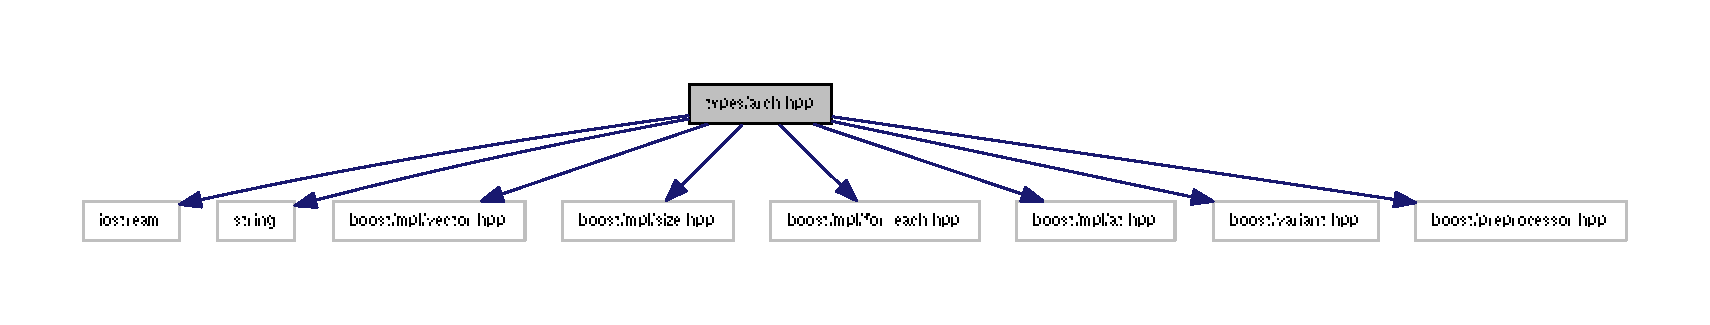
\includegraphics[width=350pt]{types_2arch_8hpp__incl}
\end{center}
\end{figure}
This graph shows which files directly or indirectly include this file\+:
\nopagebreak
\begin{figure}[H]
\begin{center}
\leavevmode
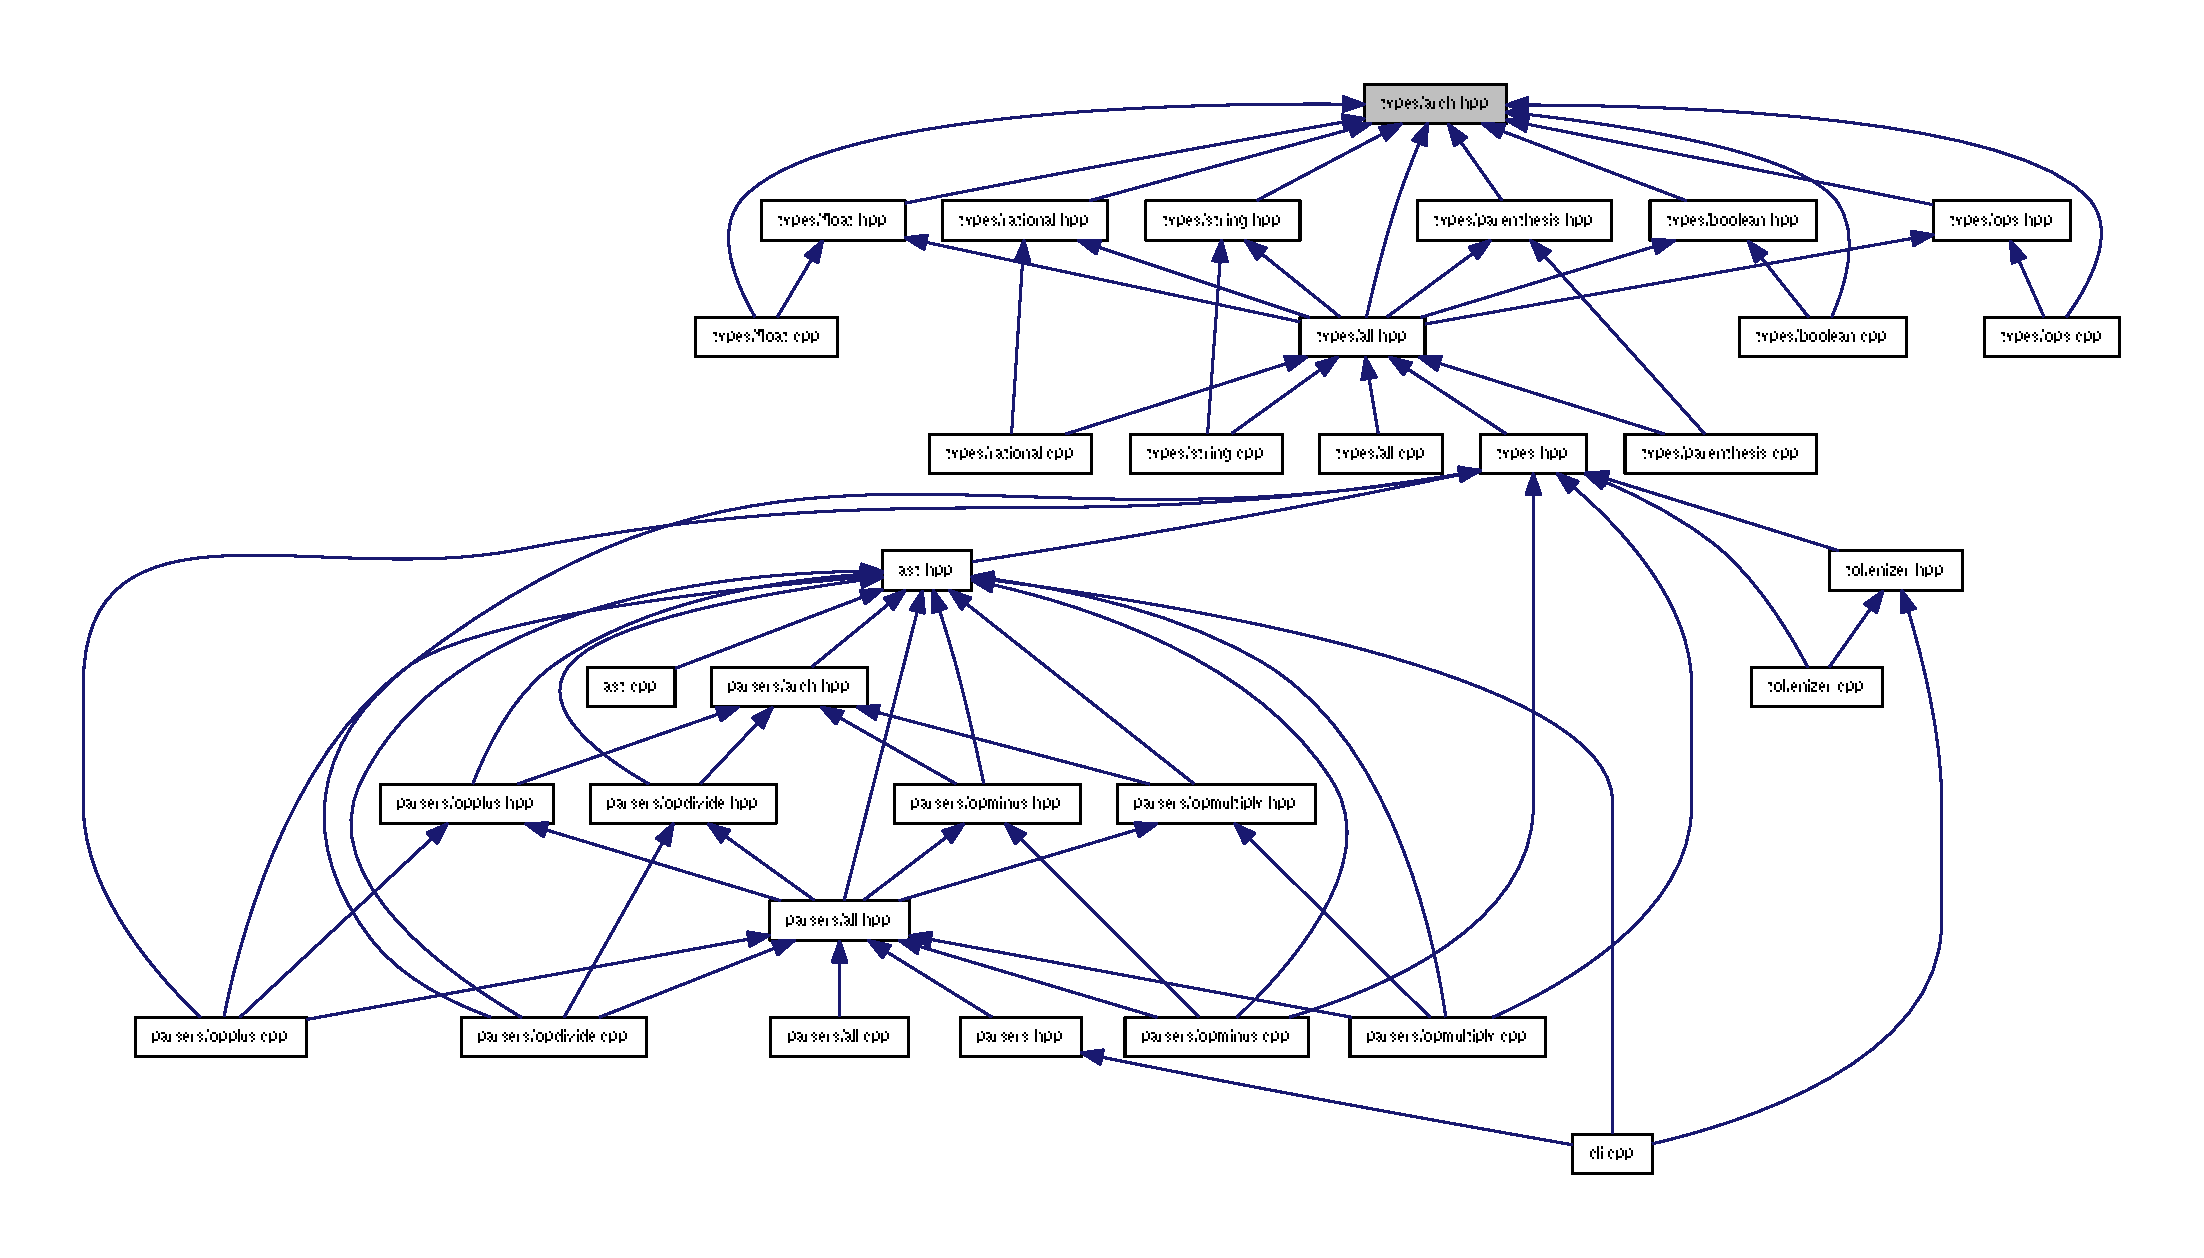
\includegraphics[width=350pt]{types_2arch_8hpp__dep__incl}
\end{center}
\end{figure}
\subsection*{Macros}
\begin{DoxyCompactItemize}
\item 
\#define \hyperlink{types_2arch_8hpp_a669f5b829a7373f20602e4c063e01d99}{P\+A\+R\+S\+E\+R\+\_\+\+D\+E\+C\+L\+A\+R\+A\+T\+I\+O\+N}(N\+A\+M\+E\+\_\+,  T\+Y\+P\+E\+\_\+,  I\+N\+F\+O\+T\+Y\+P\+E\+\_\+)
\end{DoxyCompactItemize}
\subsection*{Enumerations}
\begin{DoxyCompactItemize}
\item 
enum \hyperlink{types_2arch_8hpp_aa520fbf142ba1e7e659590c07da31921}{Token\+Type} \{ \\*
\hyperlink{types_2arch_8hpp_aa520fbf142ba1e7e659590c07da31921a0e229922772e1ebbe231bb76b1d0674e}{Left\+Parenthesis}, 
\hyperlink{types_2arch_8hpp_aa520fbf142ba1e7e659590c07da31921aa6ae499ba91edf718de60cefdb91e070}{Right\+Parenthesis}, 
\hyperlink{types_2arch_8hpp_aa520fbf142ba1e7e659590c07da31921a553e6f09de6793cb7e48368fae2c7afe}{Op\+Plus}, 
\hyperlink{types_2arch_8hpp_aa520fbf142ba1e7e659590c07da31921aaa3c8287ef3b1b2f65ca22def9d514c8}{Op\+Minus}, 
\\*
\hyperlink{types_2arch_8hpp_aa520fbf142ba1e7e659590c07da31921aa18a9690cbc2e7c5e8df90b8278b9221}{Op\+Multiply}, 
\hyperlink{types_2arch_8hpp_aa520fbf142ba1e7e659590c07da31921a6271add987abf4c1f4c420ffa7b505ac}{Op\+Divide}, 
\hyperlink{types_2arch_8hpp_aa520fbf142ba1e7e659590c07da31921ad67b0ee7230dcecb610254e4e5e589cd}{Float}, 
\hyperlink{types_2arch_8hpp_aa520fbf142ba1e7e659590c07da31921ac484461d6c31e2ef0d6ea82009ad1575}{Rational}, 
\\*
\hyperlink{types_2arch_8hpp_aa520fbf142ba1e7e659590c07da31921ade17ec82ff106e0c2b4417f5ca231eae}{String}, 
\hyperlink{types_2arch_8hpp_aa520fbf142ba1e7e659590c07da31921a3e74f2723415f1cc3cc2f3883f68add8}{Boolean}
 \}
\end{DoxyCompactItemize}


\subsection{Macro Definition Documentation}
\hypertarget{types_2arch_8hpp_a669f5b829a7373f20602e4c063e01d99}{}\index{types/arch.\+hpp@{types/arch.\+hpp}!P\+A\+R\+S\+E\+R\+\_\+\+D\+E\+C\+L\+A\+R\+A\+T\+I\+O\+N@{P\+A\+R\+S\+E\+R\+\_\+\+D\+E\+C\+L\+A\+R\+A\+T\+I\+O\+N}}
\index{P\+A\+R\+S\+E\+R\+\_\+\+D\+E\+C\+L\+A\+R\+A\+T\+I\+O\+N@{P\+A\+R\+S\+E\+R\+\_\+\+D\+E\+C\+L\+A\+R\+A\+T\+I\+O\+N}!types/arch.\+hpp@{types/arch.\+hpp}}
\subsubsection[{P\+A\+R\+S\+E\+R\+\_\+\+D\+E\+C\+L\+A\+R\+A\+T\+I\+O\+N}]{\setlength{\rightskip}{0pt plus 5cm}\#define P\+A\+R\+S\+E\+R\+\_\+\+D\+E\+C\+L\+A\+R\+A\+T\+I\+O\+N(
\begin{DoxyParamCaption}
\item[{}]{N\+A\+M\+E\+\_\+, }
\item[{}]{T\+Y\+P\+E\+\_\+, }
\item[{}]{I\+N\+F\+O\+T\+Y\+P\+E\+\_\+}
\end{DoxyParamCaption}
)}\label{types_2arch_8hpp_a669f5b829a7373f20602e4c063e01d99}
{\bfseries Value\+:}
\begin{DoxyCode}
\textcolor{keyword}{struct }NAME\_ \(\backslash\)
\{               \(\backslash\)
    typedef INFOTYPE\_ InfoType; \(\backslash\)
    static \textcolor{keyword}{const} \hyperlink{types_2arch_8hpp_aa520fbf142ba1e7e659590c07da31921}{TokenType} type;      \(\backslash\)
    static \textcolor{keywordtype}{bool} judge(\textcolor{keyword}{const} std::string& token); \(\backslash\)
    static InfoType \textcolor{keyword}{get}(\textcolor{keyword}{const} std::string& token);  \(\backslash\)
\};
\end{DoxyCode}


Definition at line 31 of file arch.\+hpp.



\subsection{Enumeration Type Documentation}
\hypertarget{types_2arch_8hpp_aa520fbf142ba1e7e659590c07da31921}{}\index{types/arch.\+hpp@{types/arch.\+hpp}!Token\+Type@{Token\+Type}}
\index{Token\+Type@{Token\+Type}!types/arch.\+hpp@{types/arch.\+hpp}}
\subsubsection[{Token\+Type}]{\setlength{\rightskip}{0pt plus 5cm}enum {\bf Token\+Type}}\label{types_2arch_8hpp_aa520fbf142ba1e7e659590c07da31921}
\begin{Desc}
\item[Enumerator]\par
\begin{description}
\index{Left\+Parenthesis@{Left\+Parenthesis}!types/arch.\+hpp@{types/arch.\+hpp}}\index{types/arch.\+hpp@{types/arch.\+hpp}!Left\+Parenthesis@{Left\+Parenthesis}}\item[{\em 
\hypertarget{types_2arch_8hpp_aa520fbf142ba1e7e659590c07da31921a0e229922772e1ebbe231bb76b1d0674e}{}Left\+Parenthesis\label{types_2arch_8hpp_aa520fbf142ba1e7e659590c07da31921a0e229922772e1ebbe231bb76b1d0674e}
}]\index{Right\+Parenthesis@{Right\+Parenthesis}!types/arch.\+hpp@{types/arch.\+hpp}}\index{types/arch.\+hpp@{types/arch.\+hpp}!Right\+Parenthesis@{Right\+Parenthesis}}\item[{\em 
\hypertarget{types_2arch_8hpp_aa520fbf142ba1e7e659590c07da31921aa6ae499ba91edf718de60cefdb91e070}{}Right\+Parenthesis\label{types_2arch_8hpp_aa520fbf142ba1e7e659590c07da31921aa6ae499ba91edf718de60cefdb91e070}
}]\index{Op\+Plus@{Op\+Plus}!types/arch.\+hpp@{types/arch.\+hpp}}\index{types/arch.\+hpp@{types/arch.\+hpp}!Op\+Plus@{Op\+Plus}}\item[{\em 
\hypertarget{types_2arch_8hpp_aa520fbf142ba1e7e659590c07da31921a553e6f09de6793cb7e48368fae2c7afe}{}Op\+Plus\label{types_2arch_8hpp_aa520fbf142ba1e7e659590c07da31921a553e6f09de6793cb7e48368fae2c7afe}
}]\index{Op\+Minus@{Op\+Minus}!types/arch.\+hpp@{types/arch.\+hpp}}\index{types/arch.\+hpp@{types/arch.\+hpp}!Op\+Minus@{Op\+Minus}}\item[{\em 
\hypertarget{types_2arch_8hpp_aa520fbf142ba1e7e659590c07da31921aaa3c8287ef3b1b2f65ca22def9d514c8}{}Op\+Minus\label{types_2arch_8hpp_aa520fbf142ba1e7e659590c07da31921aaa3c8287ef3b1b2f65ca22def9d514c8}
}]\index{Op\+Multiply@{Op\+Multiply}!types/arch.\+hpp@{types/arch.\+hpp}}\index{types/arch.\+hpp@{types/arch.\+hpp}!Op\+Multiply@{Op\+Multiply}}\item[{\em 
\hypertarget{types_2arch_8hpp_aa520fbf142ba1e7e659590c07da31921aa18a9690cbc2e7c5e8df90b8278b9221}{}Op\+Multiply\label{types_2arch_8hpp_aa520fbf142ba1e7e659590c07da31921aa18a9690cbc2e7c5e8df90b8278b9221}
}]\index{Op\+Divide@{Op\+Divide}!types/arch.\+hpp@{types/arch.\+hpp}}\index{types/arch.\+hpp@{types/arch.\+hpp}!Op\+Divide@{Op\+Divide}}\item[{\em 
\hypertarget{types_2arch_8hpp_aa520fbf142ba1e7e659590c07da31921a6271add987abf4c1f4c420ffa7b505ac}{}Op\+Divide\label{types_2arch_8hpp_aa520fbf142ba1e7e659590c07da31921a6271add987abf4c1f4c420ffa7b505ac}
}]\index{Float@{Float}!types/arch.\+hpp@{types/arch.\+hpp}}\index{types/arch.\+hpp@{types/arch.\+hpp}!Float@{Float}}\item[{\em 
\hypertarget{types_2arch_8hpp_aa520fbf142ba1e7e659590c07da31921ad67b0ee7230dcecb610254e4e5e589cd}{}Float\label{types_2arch_8hpp_aa520fbf142ba1e7e659590c07da31921ad67b0ee7230dcecb610254e4e5e589cd}
}]\index{Rational@{Rational}!types/arch.\+hpp@{types/arch.\+hpp}}\index{types/arch.\+hpp@{types/arch.\+hpp}!Rational@{Rational}}\item[{\em 
\hypertarget{types_2arch_8hpp_aa520fbf142ba1e7e659590c07da31921ac484461d6c31e2ef0d6ea82009ad1575}{}Rational\label{types_2arch_8hpp_aa520fbf142ba1e7e659590c07da31921ac484461d6c31e2ef0d6ea82009ad1575}
}]\index{String@{String}!types/arch.\+hpp@{types/arch.\+hpp}}\index{types/arch.\+hpp@{types/arch.\+hpp}!String@{String}}\item[{\em 
\hypertarget{types_2arch_8hpp_aa520fbf142ba1e7e659590c07da31921ade17ec82ff106e0c2b4417f5ca231eae}{}String\label{types_2arch_8hpp_aa520fbf142ba1e7e659590c07da31921ade17ec82ff106e0c2b4417f5ca231eae}
}]\index{Boolean@{Boolean}!types/arch.\+hpp@{types/arch.\+hpp}}\index{types/arch.\+hpp@{types/arch.\+hpp}!Boolean@{Boolean}}\item[{\em 
\hypertarget{types_2arch_8hpp_aa520fbf142ba1e7e659590c07da31921a3e74f2723415f1cc3cc2f3883f68add8}{}Boolean\label{types_2arch_8hpp_aa520fbf142ba1e7e659590c07da31921a3e74f2723415f1cc3cc2f3883f68add8}
}]\end{description}
\end{Desc}


Definition at line 17 of file arch.\+hpp.


\hypertarget{opminus_8cpp}{}\section{parsers/opminus.cpp File Reference}
\label{opminus_8cpp}\index{parsers/opminus.\+cpp@{parsers/opminus.\+cpp}}
{\ttfamily \#include \char`\"{}opminus.\+hpp\char`\"{}}\\*
{\ttfamily \#include \char`\"{}ast.\+hpp\char`\"{}}\\*
{\ttfamily \#include \char`\"{}all.\+hpp\char`\"{}}\\*
{\ttfamily \#include \char`\"{}types.\+hpp\char`\"{}}\\*
{\ttfamily \#include $<$algorithm$>$}\\*
{\ttfamily \#include $<$cassert$>$}\\*
{\ttfamily \#include $<$stdexcept$>$}\\*
{\ttfamily \#include $<$string$>$}\\*
Include dependency graph for opminus.\+cpp\+:
\nopagebreak
\begin{figure}[H]
\begin{center}
\leavevmode
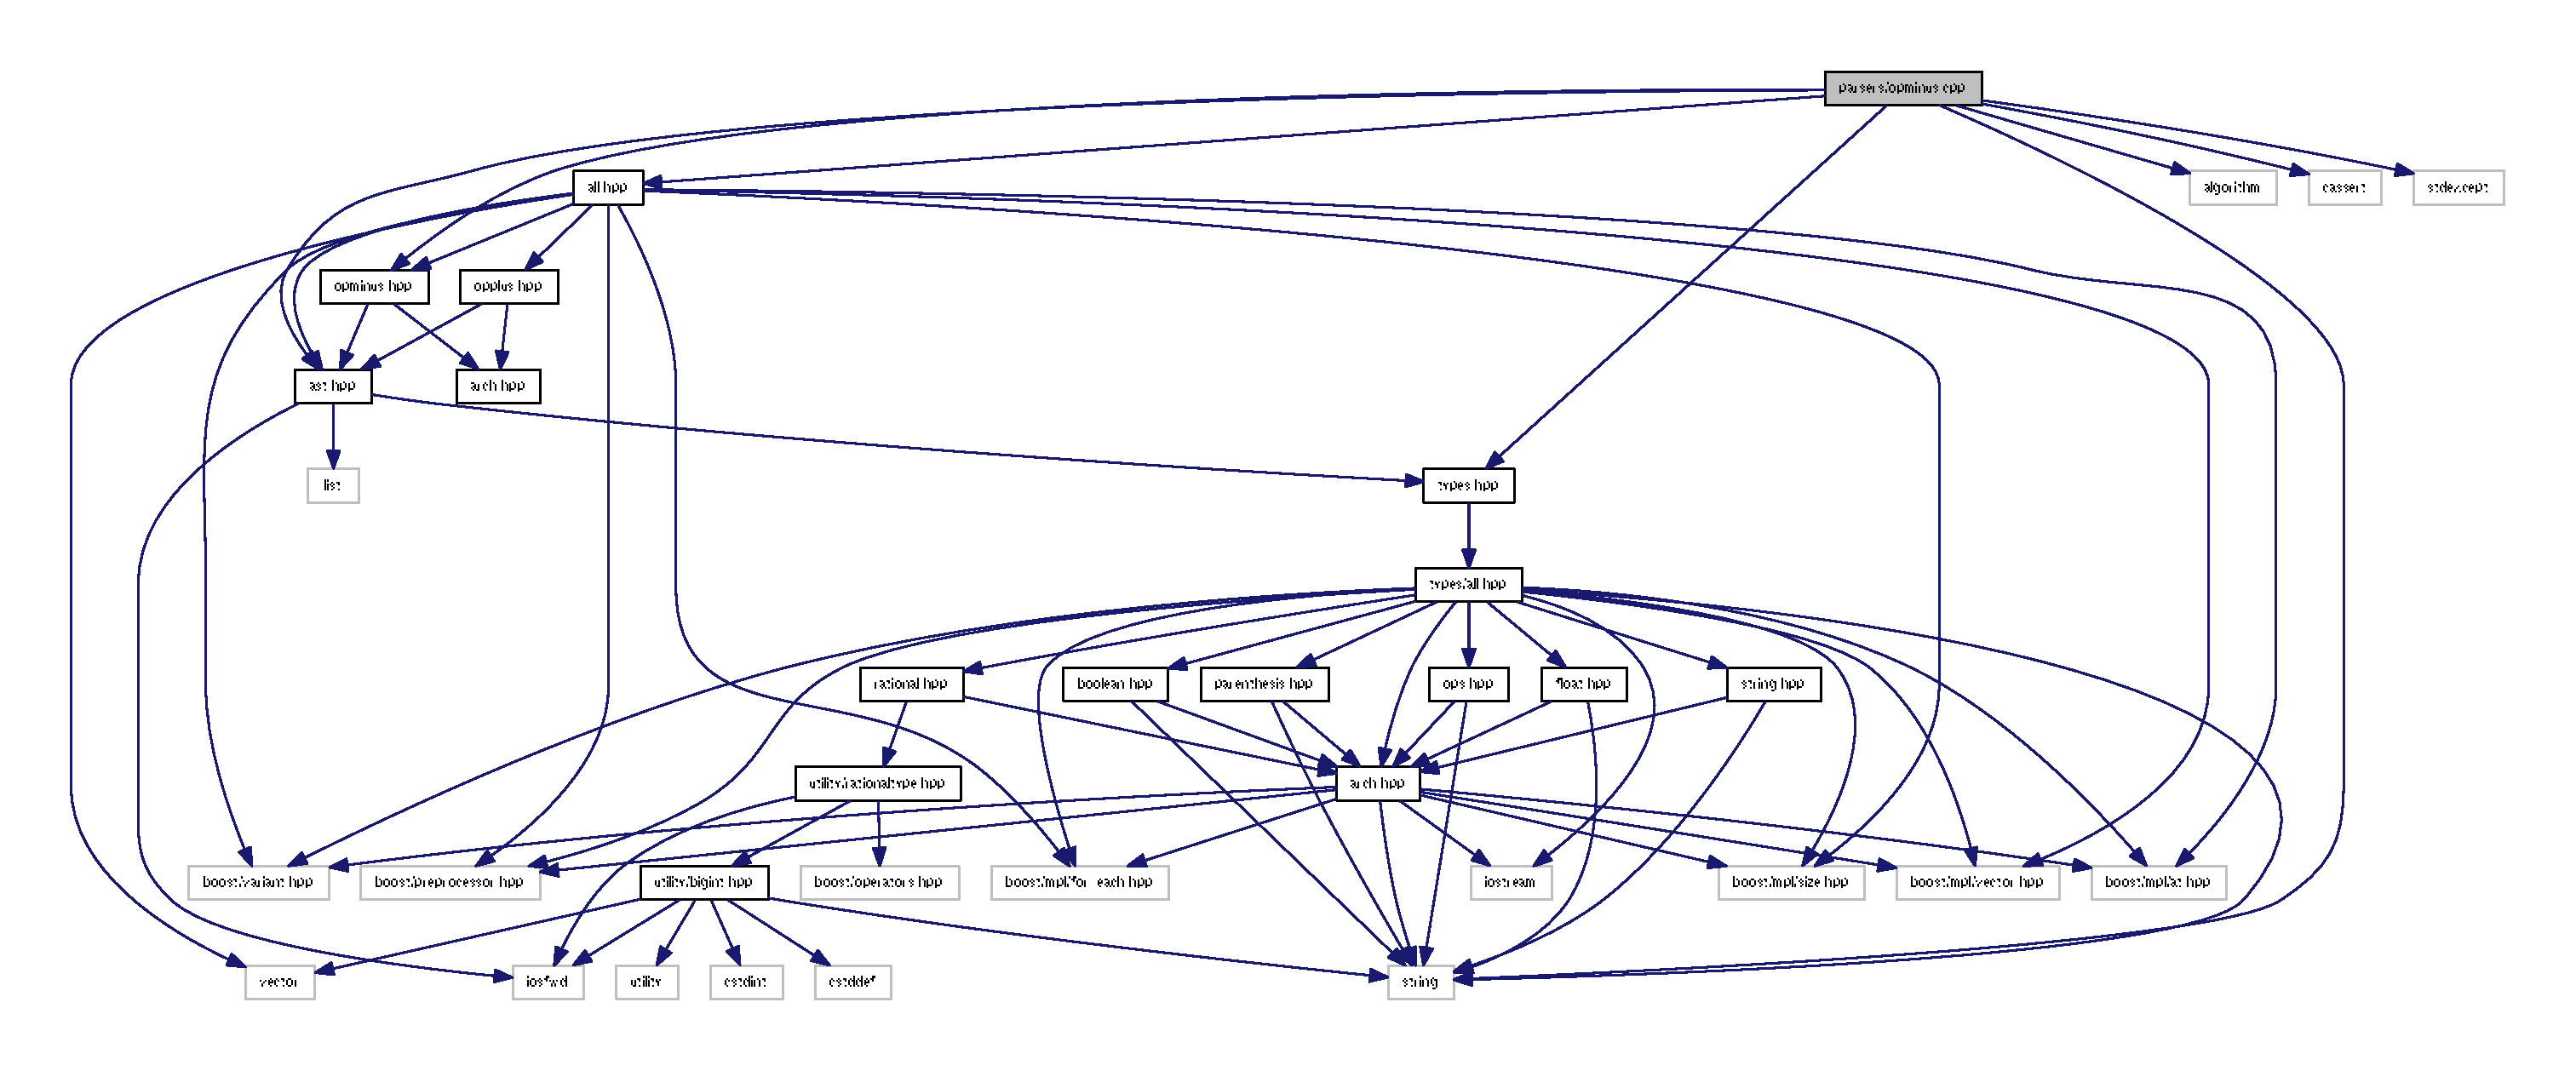
\includegraphics[width=350pt]{opminus_8cpp__incl}
\end{center}
\end{figure}

\hypertarget{opminus_8hpp}{}\section{parsers/opminus.hpp File Reference}
\label{opminus_8hpp}\index{parsers/opminus.\+hpp@{parsers/opminus.\+hpp}}
{\ttfamily \#include \char`\"{}ast.\+hpp\char`\"{}}\\*
{\ttfamily \#include \char`\"{}arch.\+hpp\char`\"{}}\\*
Include dependency graph for opminus.\+hpp\+:
\nopagebreak
\begin{figure}[H]
\begin{center}
\leavevmode
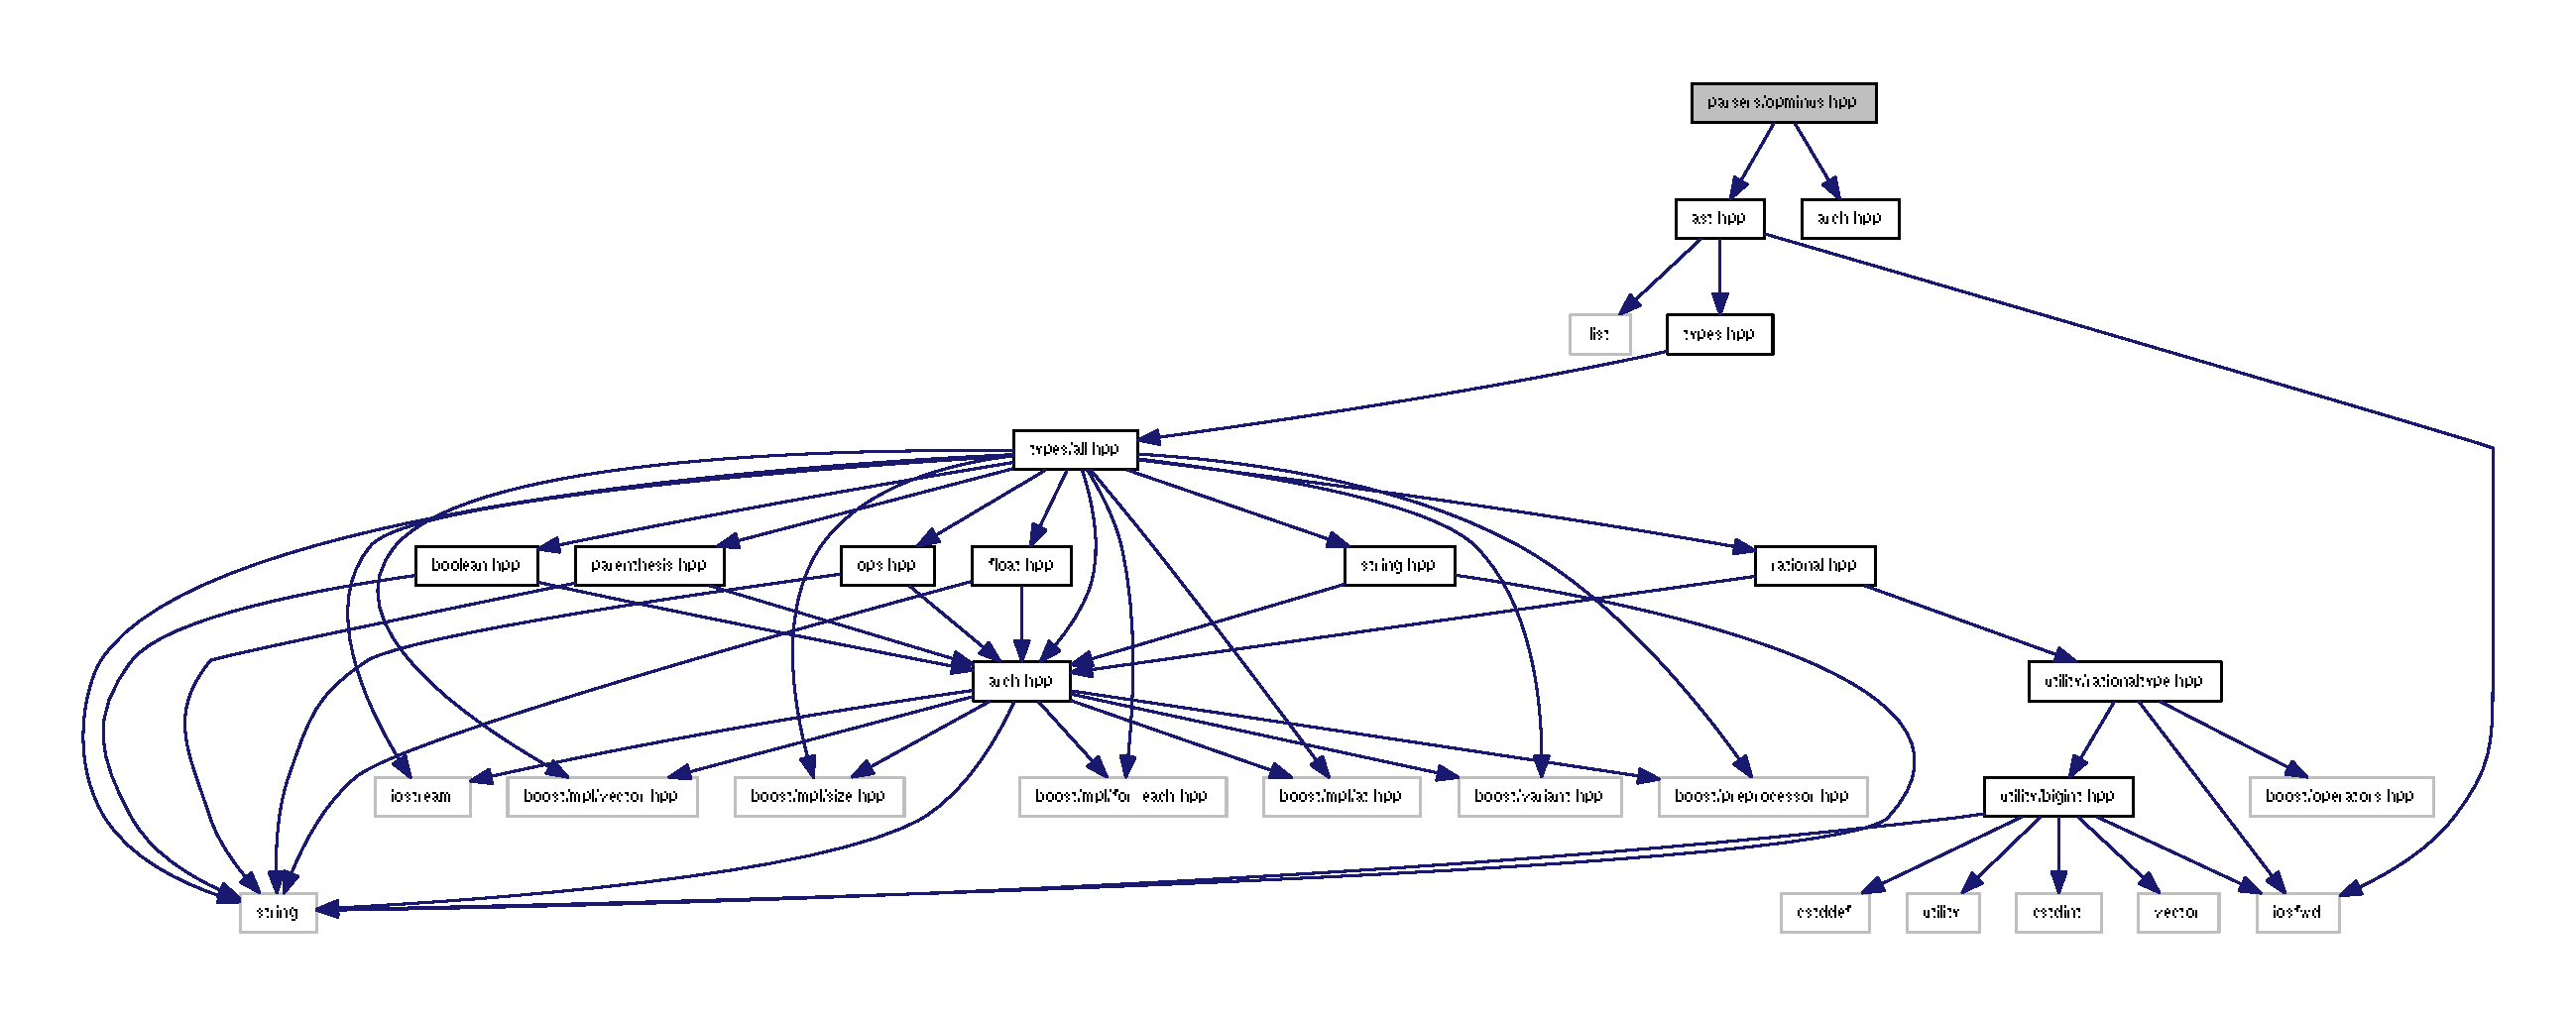
\includegraphics[width=350pt]{opminus_8hpp__incl}
\end{center}
\end{figure}
This graph shows which files directly or indirectly include this file\+:
\nopagebreak
\begin{figure}[H]
\begin{center}
\leavevmode
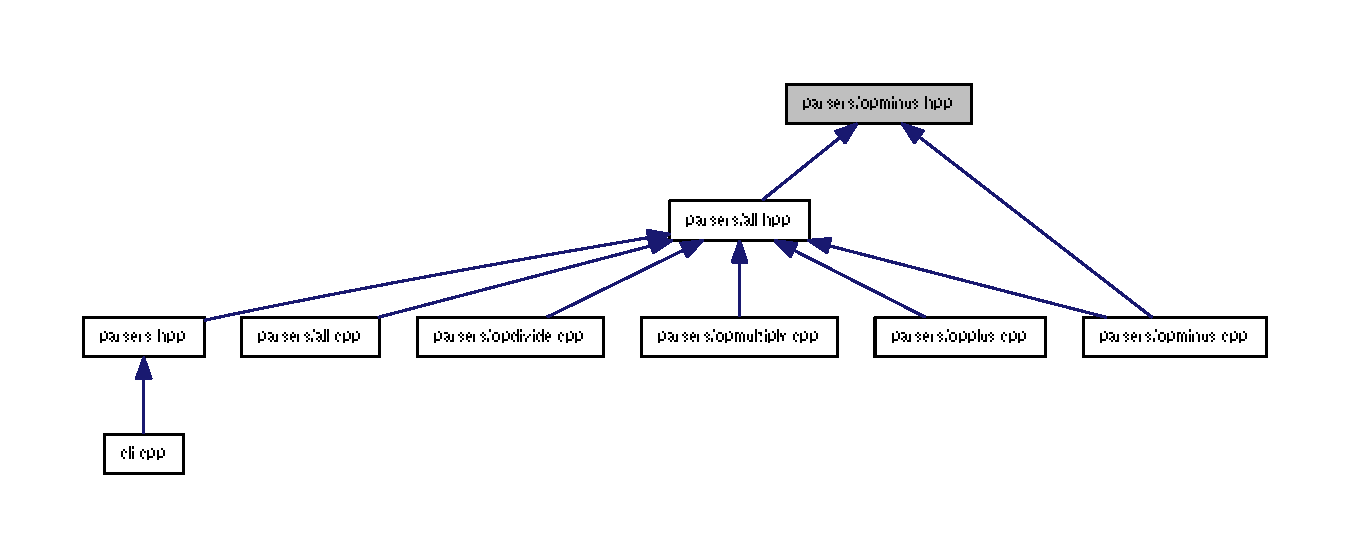
\includegraphics[width=350pt]{opminus_8hpp__dep__incl}
\end{center}
\end{figure}
\subsection*{Classes}
\begin{DoxyCompactItemize}
\item 
class \hyperlink{class_op_minus_a_s_t_parser}{Op\+Minus\+A\+S\+T\+Parser}
\end{DoxyCompactItemize}

\hypertarget{opplus_8cpp}{}\section{parsers/opplus.cpp File Reference}
\label{opplus_8cpp}\index{parsers/opplus.\+cpp@{parsers/opplus.\+cpp}}
{\ttfamily \#include \char`\"{}opplus.\+hpp\char`\"{}}\\*
{\ttfamily \#include \char`\"{}ast.\+hpp\char`\"{}}\\*
{\ttfamily \#include \char`\"{}all.\+hpp\char`\"{}}\\*
{\ttfamily \#include \char`\"{}types.\+hpp\char`\"{}}\\*
{\ttfamily \#include $<$algorithm$>$}\\*
{\ttfamily \#include $<$cassert$>$}\\*
{\ttfamily \#include $<$string$>$}\\*
{\ttfamily \#include $<$stdexcept$>$}\\*
Include dependency graph for opplus.\+cpp\+:
\nopagebreak
\begin{figure}[H]
\begin{center}
\leavevmode
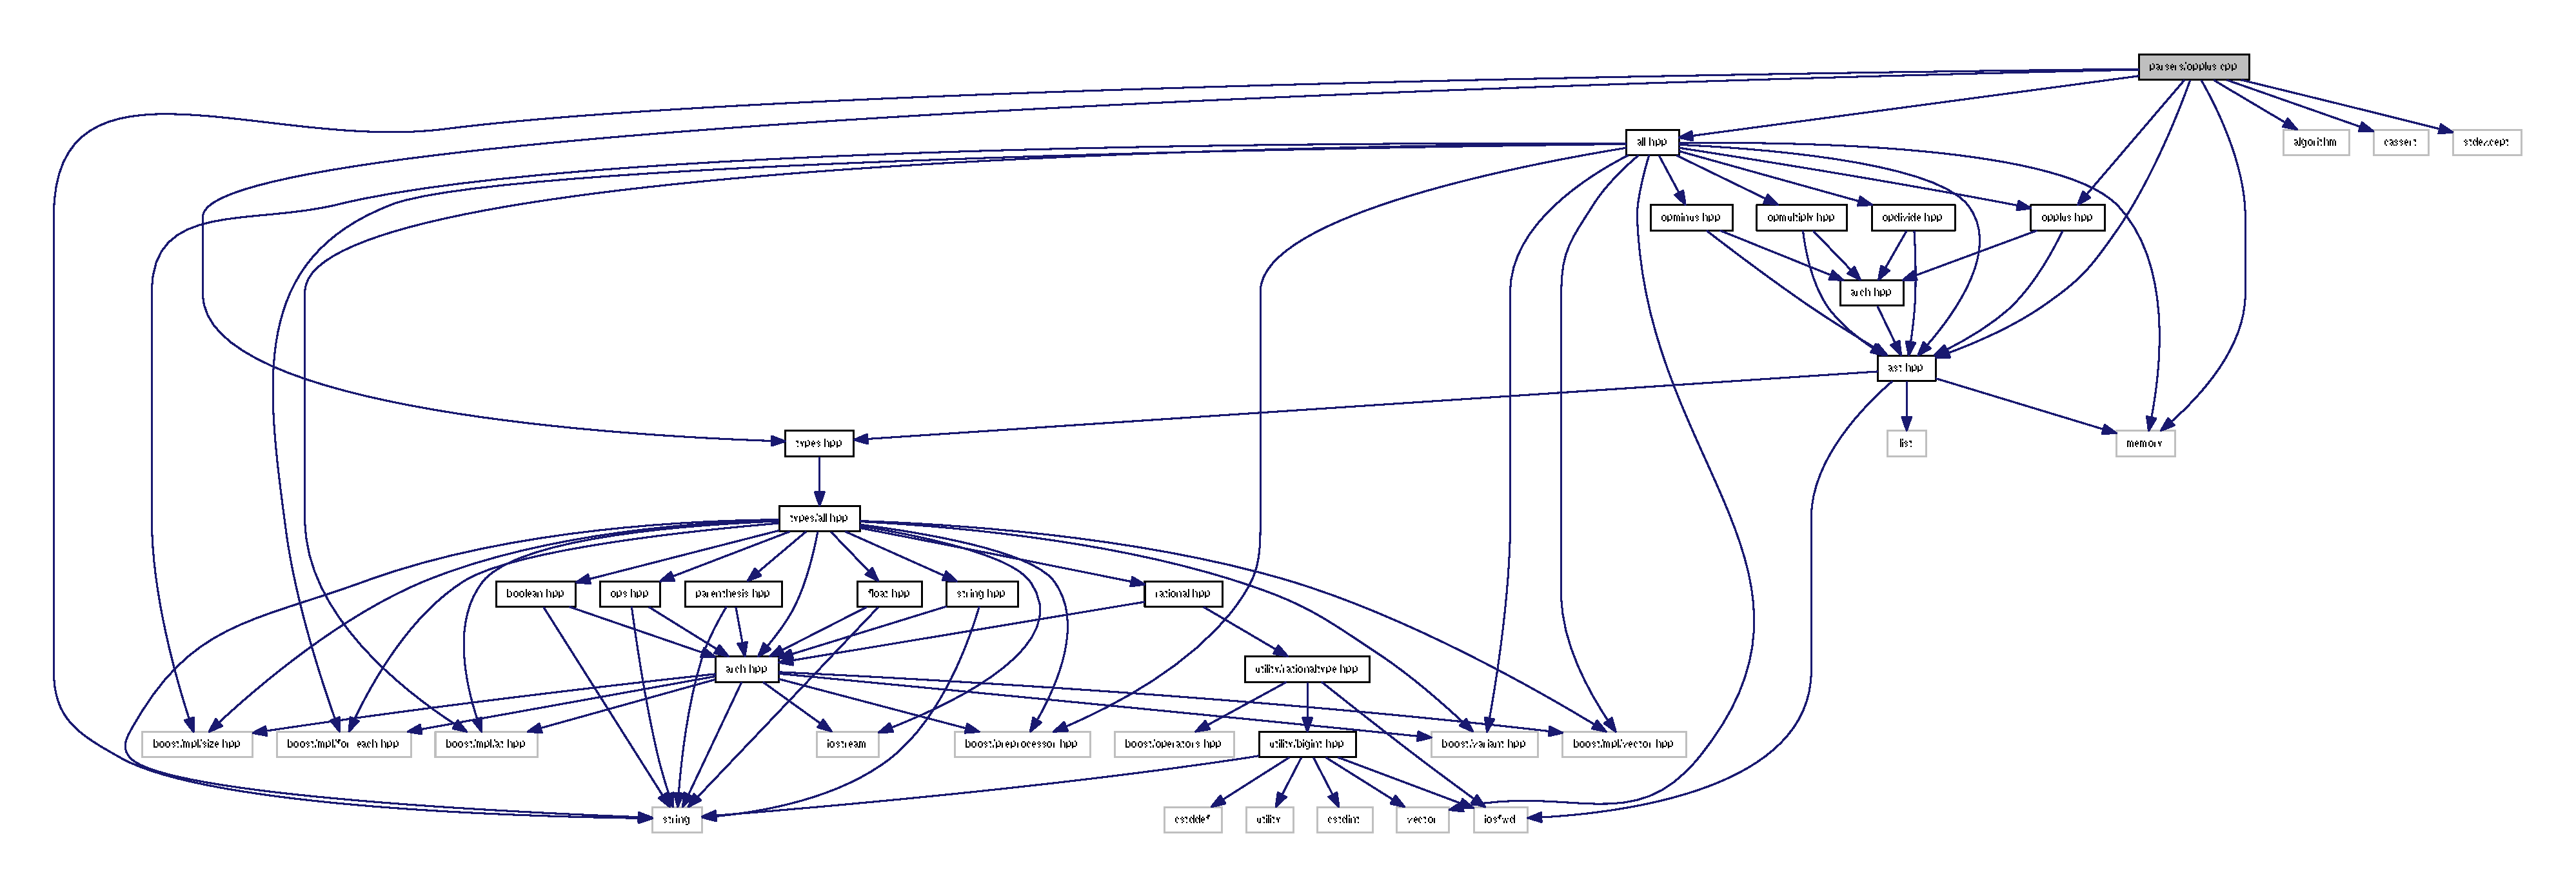
\includegraphics[width=350pt]{opplus_8cpp__incl}
\end{center}
\end{figure}

\hypertarget{opplus_8hpp}{}\section{parsers/opplus.hpp File Reference}
\label{opplus_8hpp}\index{parsers/opplus.\+hpp@{parsers/opplus.\+hpp}}
{\ttfamily \#include \char`\"{}ast.\+hpp\char`\"{}}\\*
{\ttfamily \#include \char`\"{}arch.\+hpp\char`\"{}}\\*
Include dependency graph for opplus.\+hpp\+:
\nopagebreak
\begin{figure}[H]
\begin{center}
\leavevmode
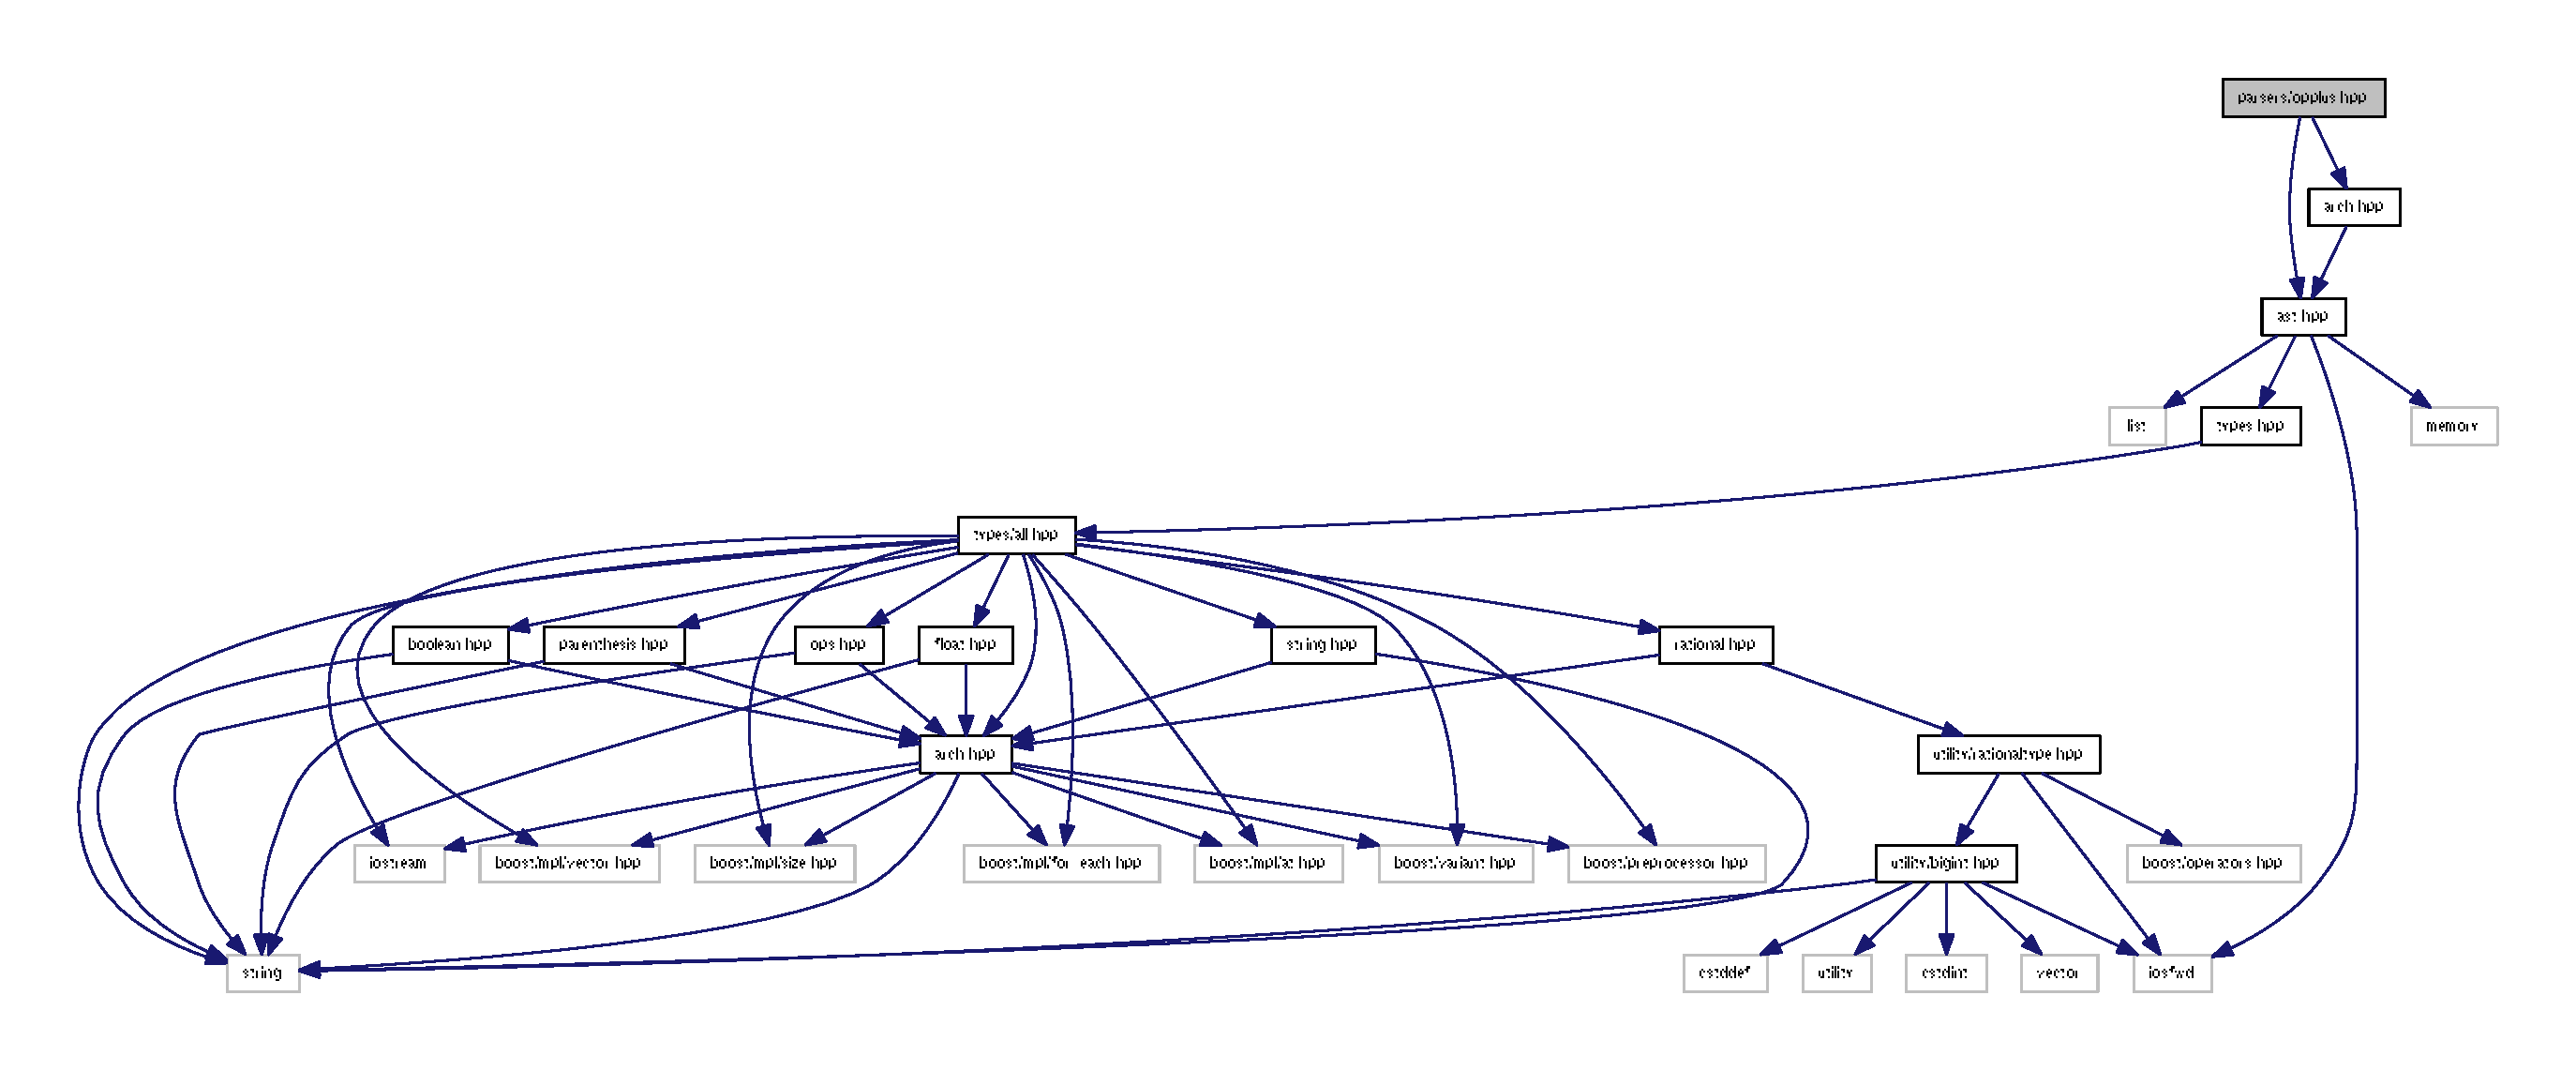
\includegraphics[width=350pt]{opplus_8hpp__incl}
\end{center}
\end{figure}
This graph shows which files directly or indirectly include this file\+:
\nopagebreak
\begin{figure}[H]
\begin{center}
\leavevmode
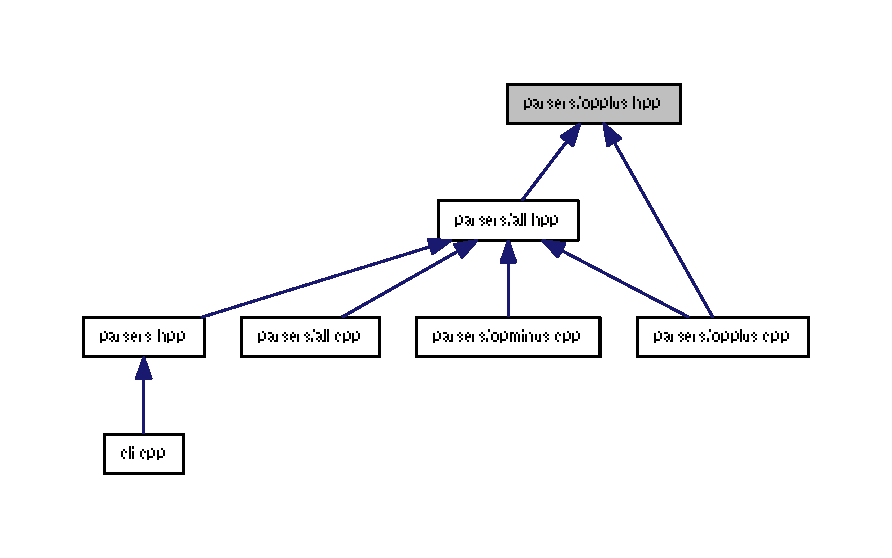
\includegraphics[width=350pt]{opplus_8hpp__dep__incl}
\end{center}
\end{figure}
\subsection*{Classes}
\begin{DoxyCompactItemize}
\item 
class \hyperlink{class_op_plus_a_s_t_parser}{Op\+Plus\+A\+S\+T\+Parser}
\end{DoxyCompactItemize}

\hypertarget{preprocessor_8cpp}{}\section{preprocessor.\+cpp File Reference}
\label{preprocessor_8cpp}\index{preprocessor.\+cpp@{preprocessor.\+cpp}}
{\ttfamily \#include $<$istream$>$}\\*
{\ttfamily \#include $<$string$>$}\\*
{\ttfamily \#include $<$cstddef$>$}\\*
{\ttfamily \#include \char`\"{}preprocessor.\+hpp\char`\"{}}\\*
Include dependency graph for preprocessor.\+cpp\+:\nopagebreak
\begin{figure}[H]
\begin{center}
\leavevmode
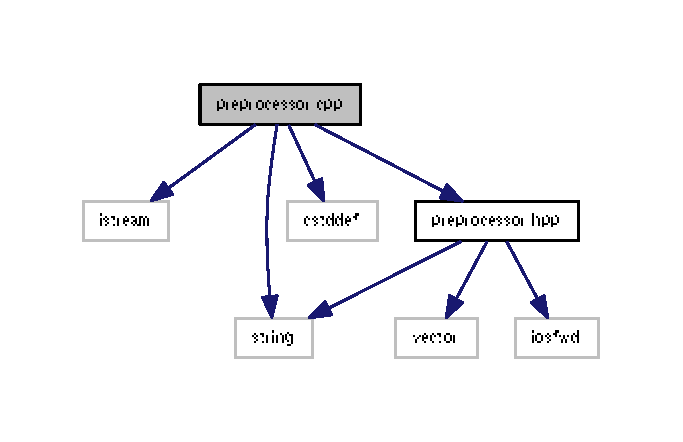
\includegraphics[width=328pt]{preprocessor_8cpp__incl}
\end{center}
\end{figure}

\hypertarget{preprocessor_8hpp}{}\section{preprocessor.\+hpp File Reference}
\label{preprocessor_8hpp}\index{preprocessor.\+hpp@{preprocessor.\+hpp}}
{\ttfamily \#include $<$string$>$}\\*
{\ttfamily \#include $<$vector$>$}\\*
{\ttfamily \#include $<$iosfwd$>$}\\*
Include dependency graph for preprocessor.\+hpp\+:\nopagebreak
\begin{figure}[H]
\begin{center}
\leavevmode
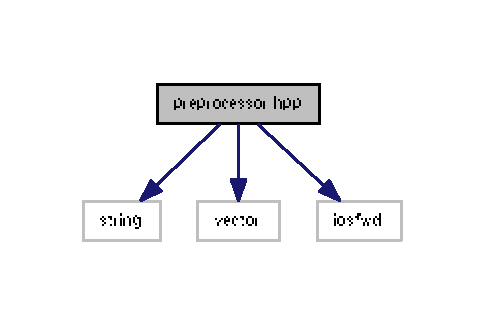
\includegraphics[width=233pt]{preprocessor_8hpp__incl}
\end{center}
\end{figure}
This graph shows which files directly or indirectly include this file\+:
\nopagebreak
\begin{figure}[H]
\begin{center}
\leavevmode
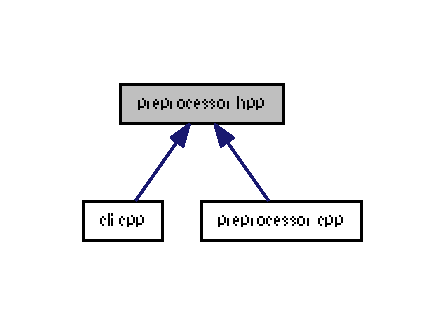
\includegraphics[width=214pt]{preprocessor_8hpp__dep__incl}
\end{center}
\end{figure}
\subsection*{Classes}
\begin{DoxyCompactItemize}
\item 
class \hyperlink{class_scheme_unit}{Scheme\+Unit}
\end{DoxyCompactItemize}

\hypertarget{_r_e_a_d_m_e_8md}{}\section{R\+E\+A\+D\+M\+E.\+md File Reference}
\label{_r_e_a_d_m_e_8md}\index{R\+E\+A\+D\+M\+E.\+md@{R\+E\+A\+D\+M\+E.\+md}}

\hypertarget{asttest_8cpp}{}\section{test/asttest.cpp File Reference}
\label{asttest_8cpp}\index{test/asttest.\+cpp@{test/asttest.\+cpp}}

\hypertarget{biginttest_8cpp}{}\section{test/biginttest.cpp File Reference}
\label{biginttest_8cpp}\index{test/biginttest.\+cpp@{test/biginttest.\+cpp}}
{\ttfamily \#include \char`\"{}utility/bigint.\+hpp\char`\"{}}\\*
{\ttfamily \#include $<$iostream$>$}\\*
{\ttfamily \#include $<$string$>$}\\*
Include dependency graph for biginttest.\+cpp\+:
\nopagebreak
\begin{figure}[H]
\begin{center}
\leavevmode
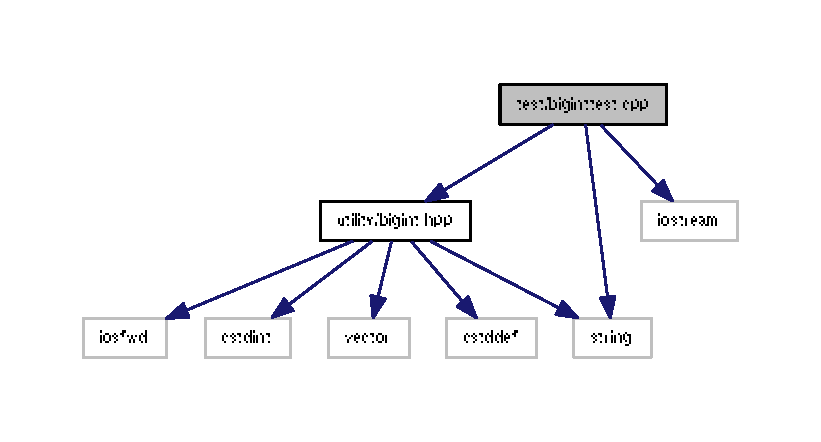
\includegraphics[width=350pt]{biginttest_8cpp__incl}
\end{center}
\end{figure}
\subsection*{Functions}
\begin{DoxyCompactItemize}
\item 
int \hyperlink{biginttest_8cpp_ae66f6b31b5ad750f1fe042a706a4e3d4}{main} ()
\end{DoxyCompactItemize}


\subsection{Function Documentation}
\hypertarget{biginttest_8cpp_ae66f6b31b5ad750f1fe042a706a4e3d4}{}\index{biginttest.\+cpp@{biginttest.\+cpp}!main@{main}}
\index{main@{main}!biginttest.\+cpp@{biginttest.\+cpp}}
\subsubsection[{main}]{\setlength{\rightskip}{0pt plus 5cm}int main (
\begin{DoxyParamCaption}
{}
\end{DoxyParamCaption}
)}\label{biginttest_8cpp_ae66f6b31b5ad750f1fe042a706a4e3d4}


Definition at line 8 of file biginttest.\+cpp.


\hypertarget{parserstest_8cpp}{}\section{test/parserstest.cpp File Reference}
\label{parserstest_8cpp}\index{test/parserstest.\+cpp@{test/parserstest.\+cpp}}

\hypertarget{preprocessortest_8cpp}{}\section{test/preprocessortest.cpp File Reference}
\label{preprocessortest_8cpp}\index{test/preprocessortest.\+cpp@{test/preprocessortest.\+cpp}}
{\ttfamily \#include \char`\"{}preprocessor.\+hpp\char`\"{}}\\*
{\ttfamily \#include $<$iostream$>$}\\*
{\ttfamily \#include $<$fstream$>$}\\*
Include dependency graph for preprocessortest.\+cpp\+:
\nopagebreak
\begin{figure}[H]
\begin{center}
\leavevmode
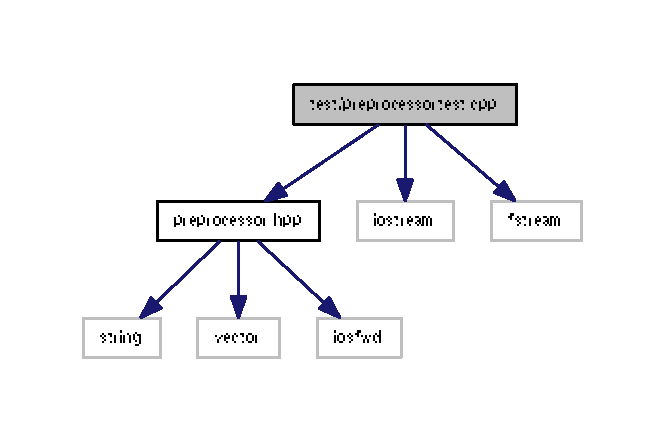
\includegraphics[width=319pt]{preprocessortest_8cpp__incl}
\end{center}
\end{figure}
\subsection*{Functions}
\begin{DoxyCompactItemize}
\item 
ifstream \hyperlink{preprocessortest_8cpp_a777949afad88957e993568613aa2dd3d}{stre} (\char`\"{}preprocessor.\+test\char`\"{})
\item 
int \hyperlink{preprocessortest_8cpp_ae66f6b31b5ad750f1fe042a706a4e3d4}{main} ()
\end{DoxyCompactItemize}
\subsection*{Variables}
\begin{DoxyCompactItemize}
\item 
\hyperlink{class_scheme_unit}{Scheme\+Unit} \hyperlink{preprocessortest_8cpp_a10d1ea193b80aa2128e080646057d11c}{s} (\hyperlink{preprocessortest_8cpp_a777949afad88957e993568613aa2dd3d}{stre})
\end{DoxyCompactItemize}


\subsection{Function Documentation}
\hypertarget{preprocessortest_8cpp_ae66f6b31b5ad750f1fe042a706a4e3d4}{}\index{preprocessortest.\+cpp@{preprocessortest.\+cpp}!main@{main}}
\index{main@{main}!preprocessortest.\+cpp@{preprocessortest.\+cpp}}
\subsubsection[{main}]{\setlength{\rightskip}{0pt plus 5cm}int main (
\begin{DoxyParamCaption}
{}
\end{DoxyParamCaption}
)}\label{preprocessortest_8cpp_ae66f6b31b5ad750f1fe042a706a4e3d4}


Definition at line 7 of file preprocessortest.\+cpp.

\hypertarget{preprocessortest_8cpp_a777949afad88957e993568613aa2dd3d}{}\index{preprocessortest.\+cpp@{preprocessortest.\+cpp}!stre@{stre}}
\index{stre@{stre}!preprocessortest.\+cpp@{preprocessortest.\+cpp}}
\subsubsection[{stre}]{\setlength{\rightskip}{0pt plus 5cm}ifstream stre (
\begin{DoxyParamCaption}
\item[{\char`\"{}preprocessor.\+test\char`\"{}}]{}
\end{DoxyParamCaption}
)}\label{preprocessortest_8cpp_a777949afad88957e993568613aa2dd3d}


\subsection{Variable Documentation}
\hypertarget{preprocessortest_8cpp_a10d1ea193b80aa2128e080646057d11c}{}\index{preprocessortest.\+cpp@{preprocessortest.\+cpp}!s@{s}}
\index{s@{s}!preprocessortest.\+cpp@{preprocessortest.\+cpp}}
\subsubsection[{s}]{\setlength{\rightskip}{0pt plus 5cm}{\bf Scheme\+Unit} s({\bf stre})}\label{preprocessortest_8cpp_a10d1ea193b80aa2128e080646057d11c}

\hypertarget{rationaltypetest_8cpp}{}\section{test/rationaltypetest.cpp File Reference}
\label{rationaltypetest_8cpp}\index{test/rationaltypetest.\+cpp@{test/rationaltypetest.\+cpp}}

\hypertarget{tokenizertest_8cpp}{}\section{test/tokenizertest.cpp File Reference}
\label{tokenizertest_8cpp}\index{test/tokenizertest.\+cpp@{test/tokenizertest.\+cpp}}
{\ttfamily \#include \char`\"{}preprocessor.\+hpp\char`\"{}}\\*
{\ttfamily \#include \char`\"{}tokenizer.\+hpp\char`\"{}}\\*
{\ttfamily \#include $<$iostream$>$}\\*
{\ttfamily \#include $<$fstream$>$}\\*
{\ttfamily \#include $<$algorithm$>$}\\*
{\ttfamily \#include $<$string$>$}\\*
Include dependency graph for tokenizertest.\+cpp\+:
\nopagebreak
\begin{figure}[H]
\begin{center}
\leavevmode
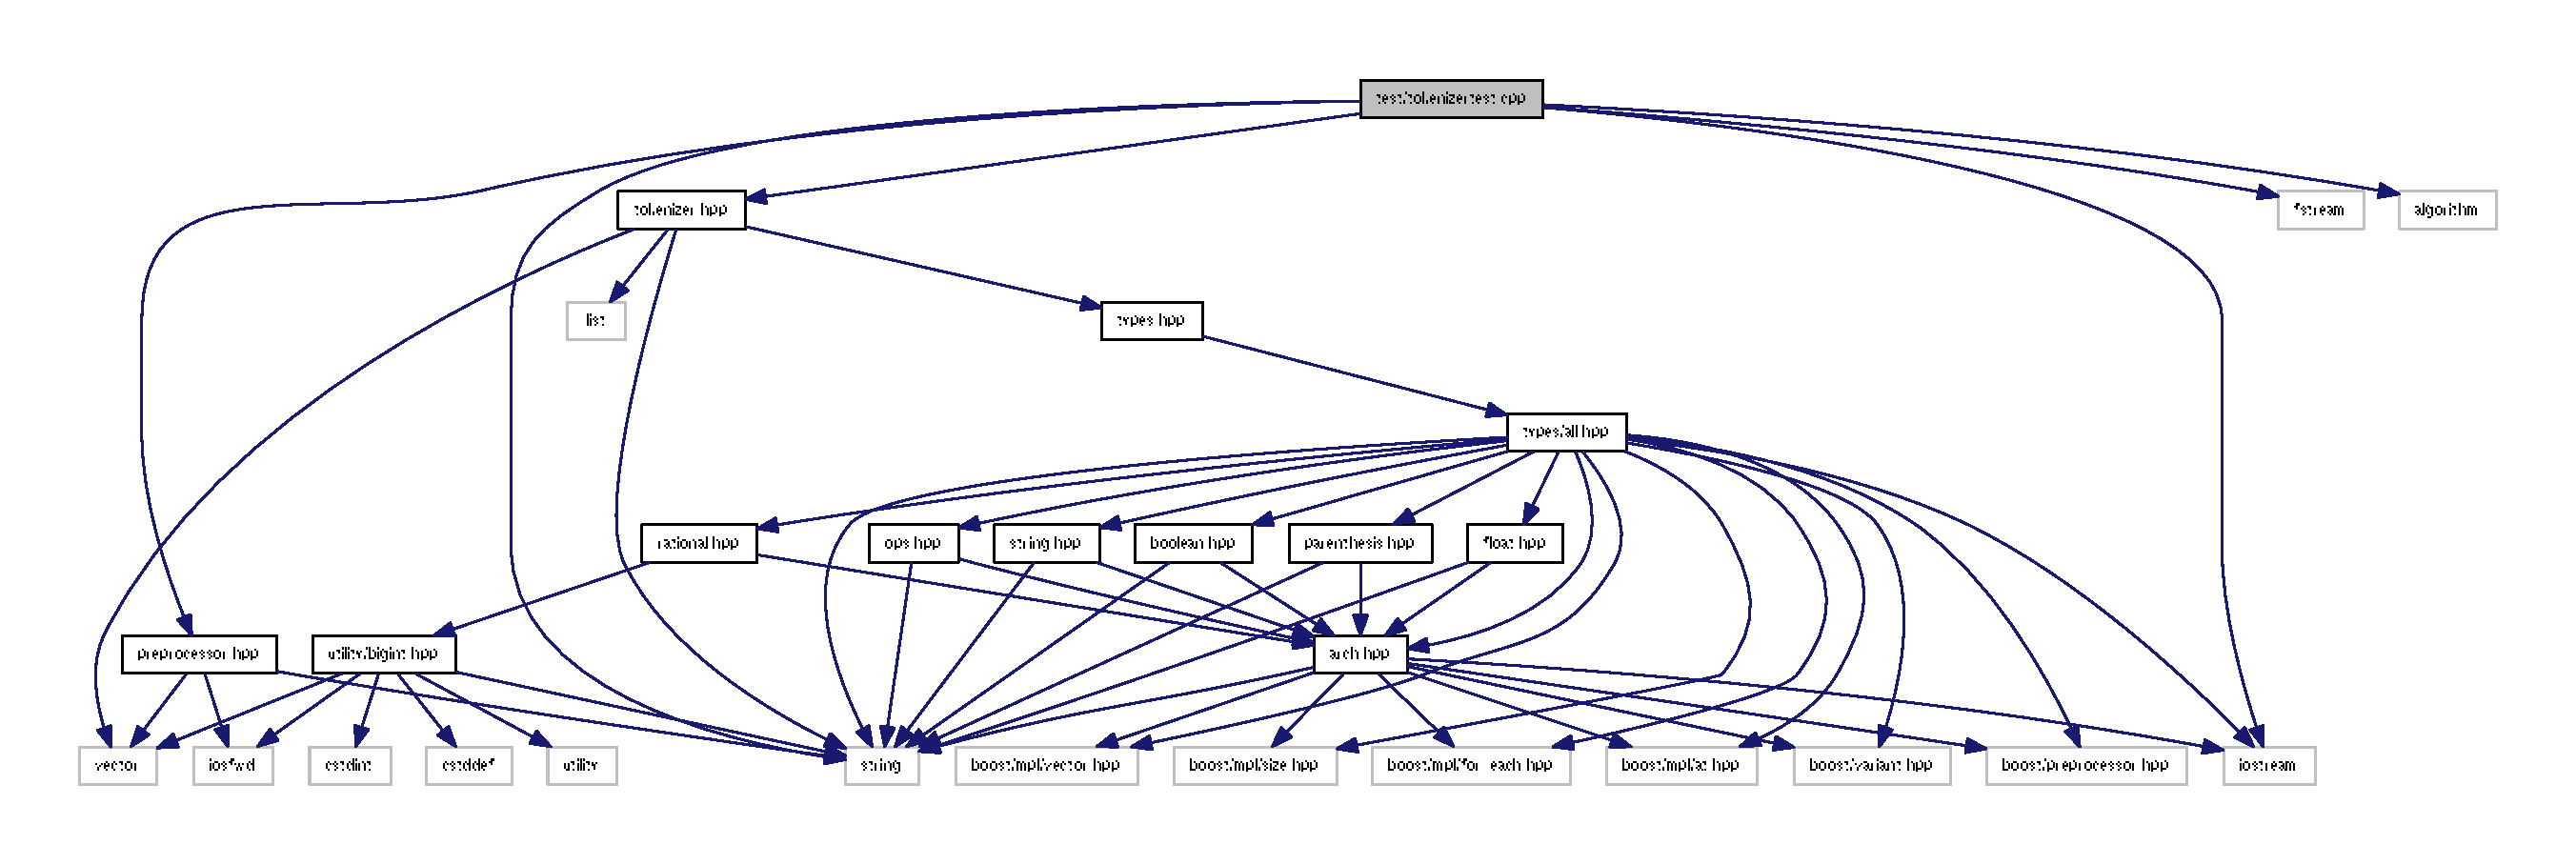
\includegraphics[width=350pt]{tokenizertest_8cpp__incl}
\end{center}
\end{figure}
\subsection*{Functions}
\begin{DoxyCompactItemize}
\item 
int \hyperlink{tokenizertest_8cpp_ae66f6b31b5ad750f1fe042a706a4e3d4}{main} ()
\end{DoxyCompactItemize}


\subsection{Function Documentation}
\hypertarget{tokenizertest_8cpp_ae66f6b31b5ad750f1fe042a706a4e3d4}{}\index{tokenizertest.\+cpp@{tokenizertest.\+cpp}!main@{main}}
\index{main@{main}!tokenizertest.\+cpp@{tokenizertest.\+cpp}}
\subsubsection[{main}]{\setlength{\rightskip}{0pt plus 5cm}int main (
\begin{DoxyParamCaption}
{}
\end{DoxyParamCaption}
)}\label{tokenizertest_8cpp_ae66f6b31b5ad750f1fe042a706a4e3d4}


Definition at line 9 of file tokenizertest.\+cpp.


\hypertarget{typestest_8cpp}{}\section{test/typestest.cpp File Reference}
\label{typestest_8cpp}\index{test/typestest.\+cpp@{test/typestest.\+cpp}}
{\ttfamily \#include \char`\"{}types.\+hpp\char`\"{}}\\*
{\ttfamily \#include $<$iostream$>$}\\*
{\ttfamily \#include $<$string$>$}\\*
Include dependency graph for typestest.\+cpp\+:
\nopagebreak
\begin{figure}[H]
\begin{center}
\leavevmode
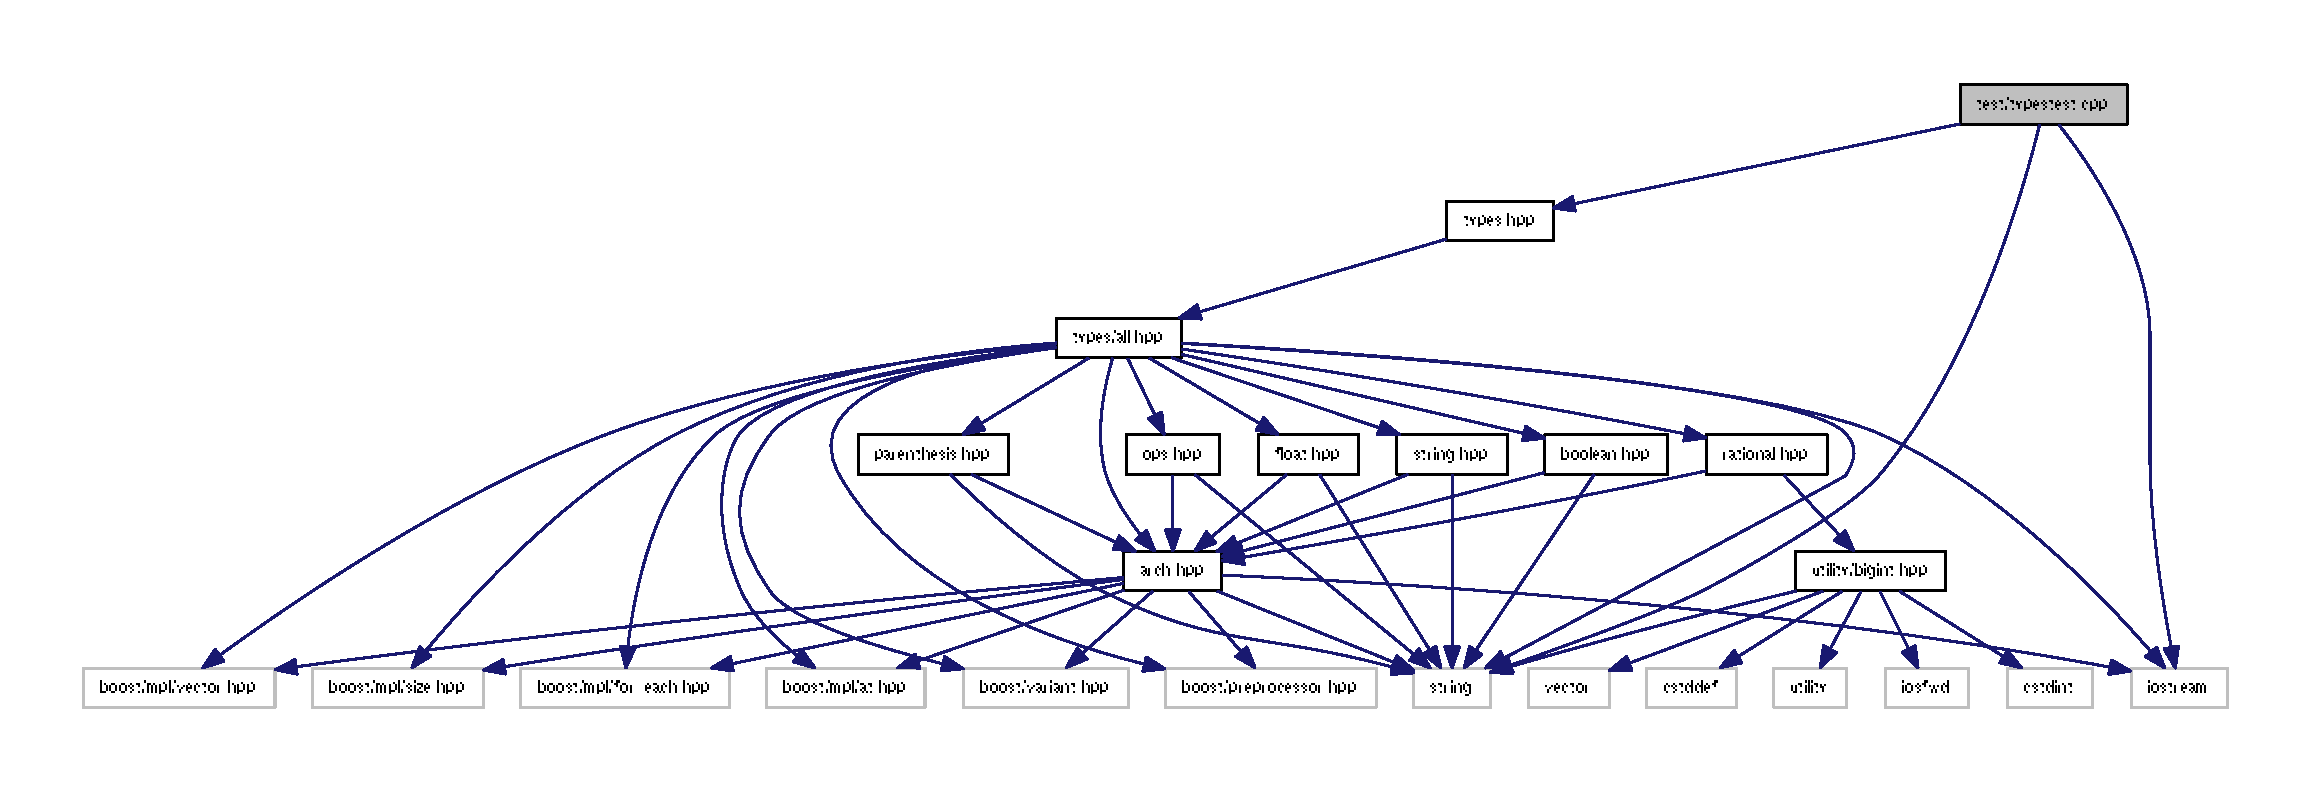
\includegraphics[width=350pt]{typestest_8cpp__incl}
\end{center}
\end{figure}
\subsection*{Functions}
\begin{DoxyCompactItemize}
\item 
int \hyperlink{typestest_8cpp_ae66f6b31b5ad750f1fe042a706a4e3d4}{main} ()
\end{DoxyCompactItemize}


\subsection{Function Documentation}
\hypertarget{typestest_8cpp_ae66f6b31b5ad750f1fe042a706a4e3d4}{}\index{typestest.\+cpp@{typestest.\+cpp}!main@{main}}
\index{main@{main}!typestest.\+cpp@{typestest.\+cpp}}
\subsubsection[{main}]{\setlength{\rightskip}{0pt plus 5cm}int main (
\begin{DoxyParamCaption}
{}
\end{DoxyParamCaption}
)}\label{typestest_8cpp_ae66f6b31b5ad750f1fe042a706a4e3d4}


Definition at line 6 of file typestest.\+cpp.


\hypertarget{tokenizer_8cpp}{}\section{tokenizer.\+cpp File Reference}
\label{tokenizer_8cpp}\index{tokenizer.\+cpp@{tokenizer.\+cpp}}
{\ttfamily \#include \char`\"{}tokenizer.\+hpp\char`\"{}}\\*
{\ttfamily \#include \char`\"{}types.\+hpp\char`\"{}}\\*
{\ttfamily \#include $<$string$>$}\\*
{\ttfamily \#include $<$vector$>$}\\*
{\ttfamily \#include $<$list$>$}\\*
{\ttfamily \#include $<$cstddef$>$}\\*
{\ttfamily \#include $<$algorithm$>$}\\*
{\ttfamily \#include $<$iostream$>$}\\*
Include dependency graph for tokenizer.\+cpp\+:
% FIG 0

\hypertarget{tokenizer_8hpp}{}\section{tokenizer.\+hpp File Reference}
\label{tokenizer_8hpp}\index{tokenizer.\+hpp@{tokenizer.\+hpp}}
{\ttfamily \#include $<$string$>$}\\*
{\ttfamily \#include $<$list$>$}\\*
{\ttfamily \#include $<$vector$>$}\\*
{\ttfamily \#include \char`\"{}types.\+hpp\char`\"{}}\\*
Include dependency graph for tokenizer.\+hpp\+:\nopagebreak
\begin{figure}[H]
\begin{center}
\leavevmode
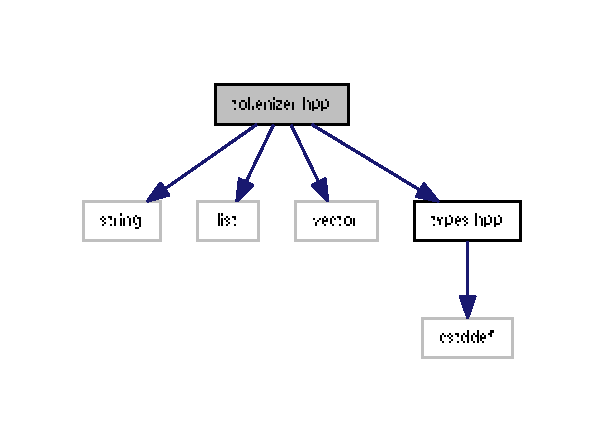
\includegraphics[width=290pt]{tokenizer_8hpp__incl}
\end{center}
\end{figure}
This graph shows which files directly or indirectly include this file\+:\nopagebreak
\begin{figure}[H]
\begin{center}
\leavevmode
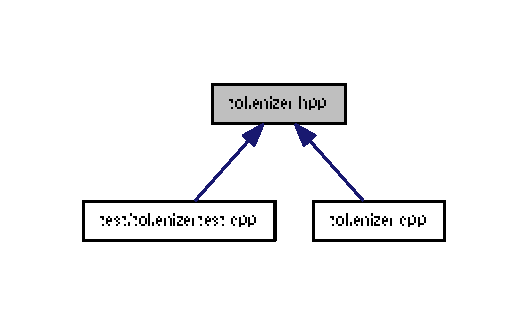
\includegraphics[width=254pt]{tokenizer_8hpp__dep__incl}
\end{center}
\end{figure}
\subsection*{Classes}
\begin{DoxyCompactItemize}
\item 
class \hyperlink{class_tokenizer}{Tokenizer}
\end{DoxyCompactItemize}

\hypertarget{types_8hpp}{}\section{types.\+hpp File Reference}
\label{types_8hpp}\index{types.\+hpp@{types.\+hpp}}
{\ttfamily \#include \char`\"{}types/all.\+hpp\char`\"{}}\\*
Include dependency graph for types.\+hpp\+:
\nopagebreak
\begin{figure}[H]
\begin{center}
\leavevmode
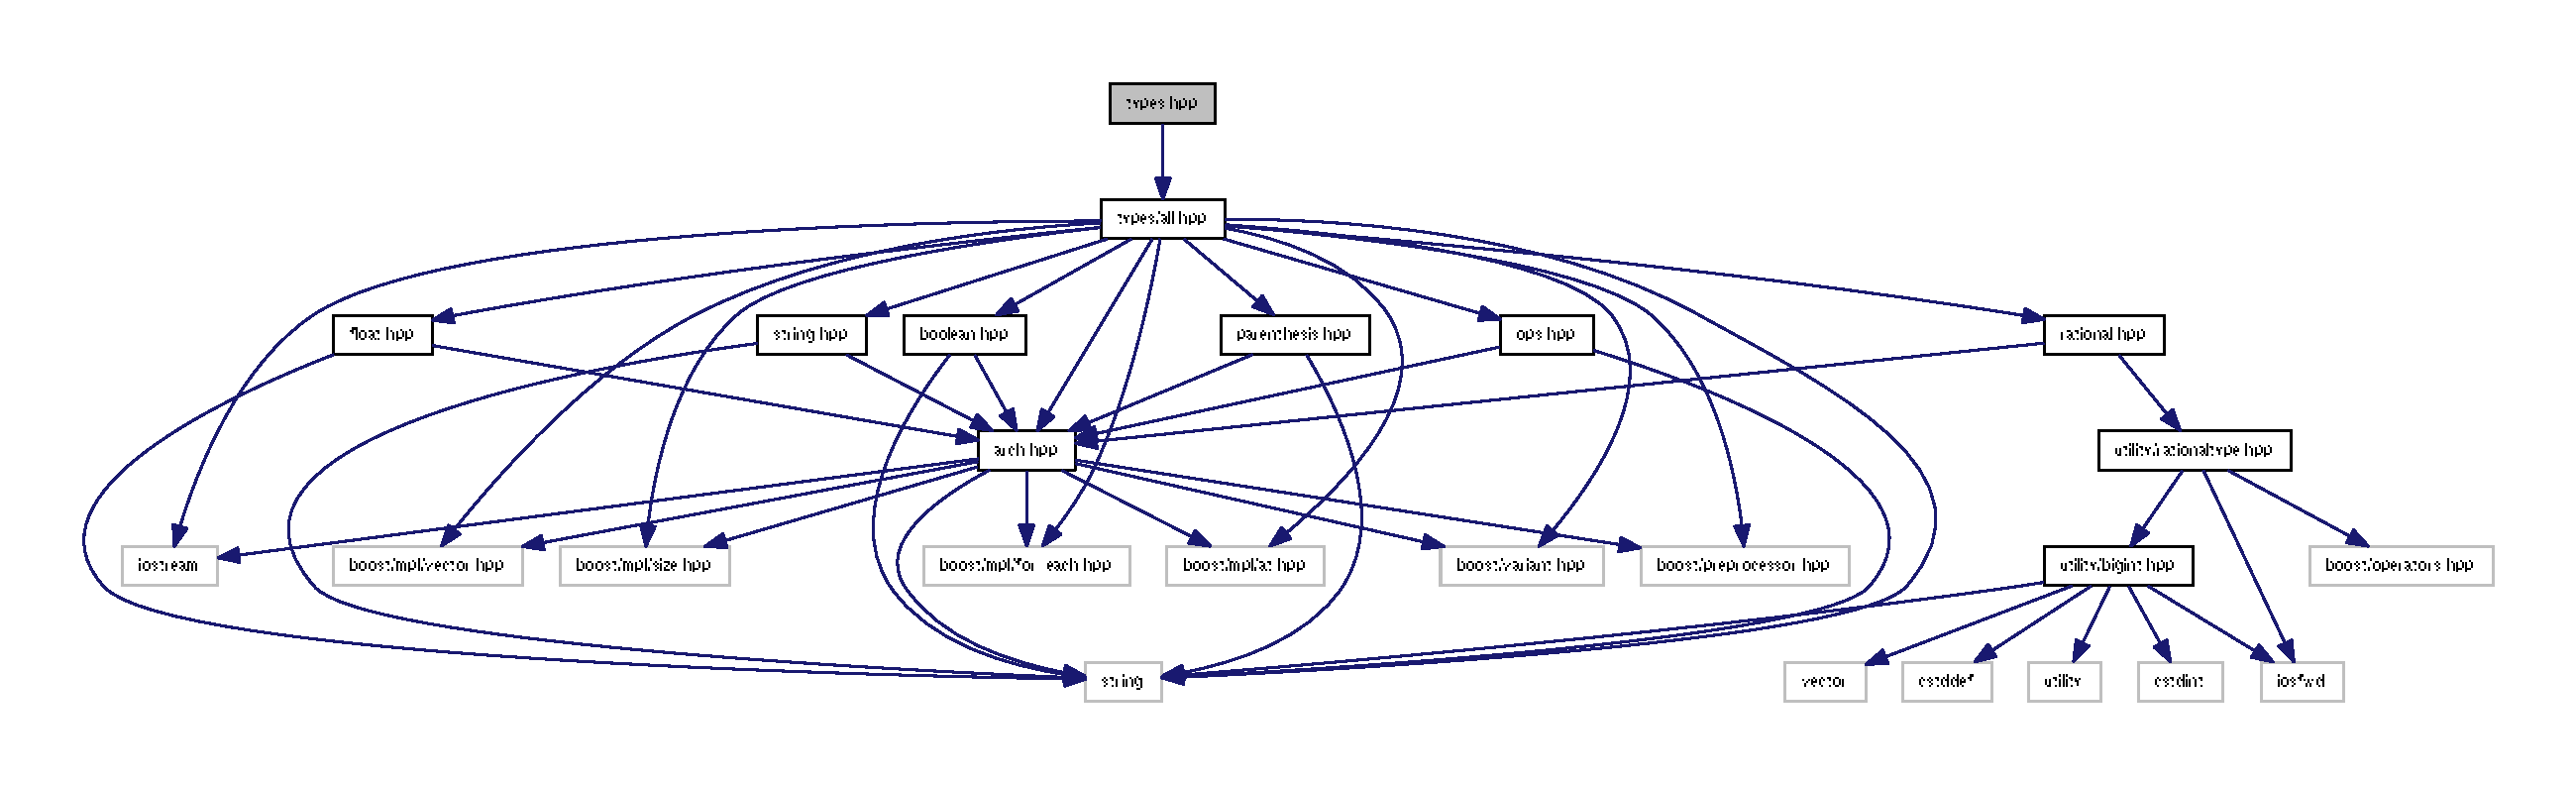
\includegraphics[width=350pt]{types_8hpp__incl}
\end{center}
\end{figure}
This graph shows which files directly or indirectly include this file\+:
\nopagebreak
\begin{figure}[H]
\begin{center}
\leavevmode
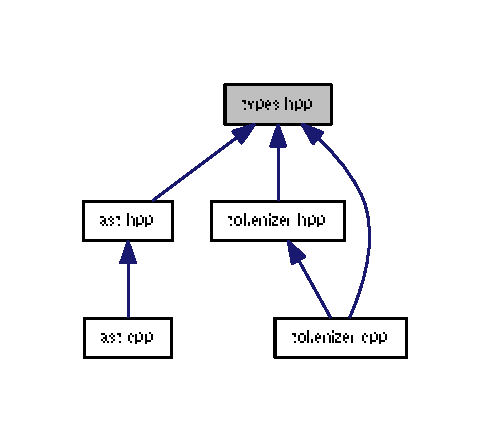
\includegraphics[width=350pt]{types_8hpp__dep__incl}
\end{center}
\end{figure}

\hypertarget{boolean_8cpp}{}\section{types/boolean.cpp File Reference}
\label{boolean_8cpp}\index{types/boolean.\+cpp@{types/boolean.\+cpp}}
{\ttfamily \#include \char`\"{}boolean.\+hpp\char`\"{}}\\*
{\ttfamily \#include \char`\"{}arch.\+hpp\char`\"{}}\\*
{\ttfamily \#include $<$string$>$}\\*
Include dependency graph for boolean.\+cpp\+:\nopagebreak
\begin{figure}[H]
\begin{center}
\leavevmode
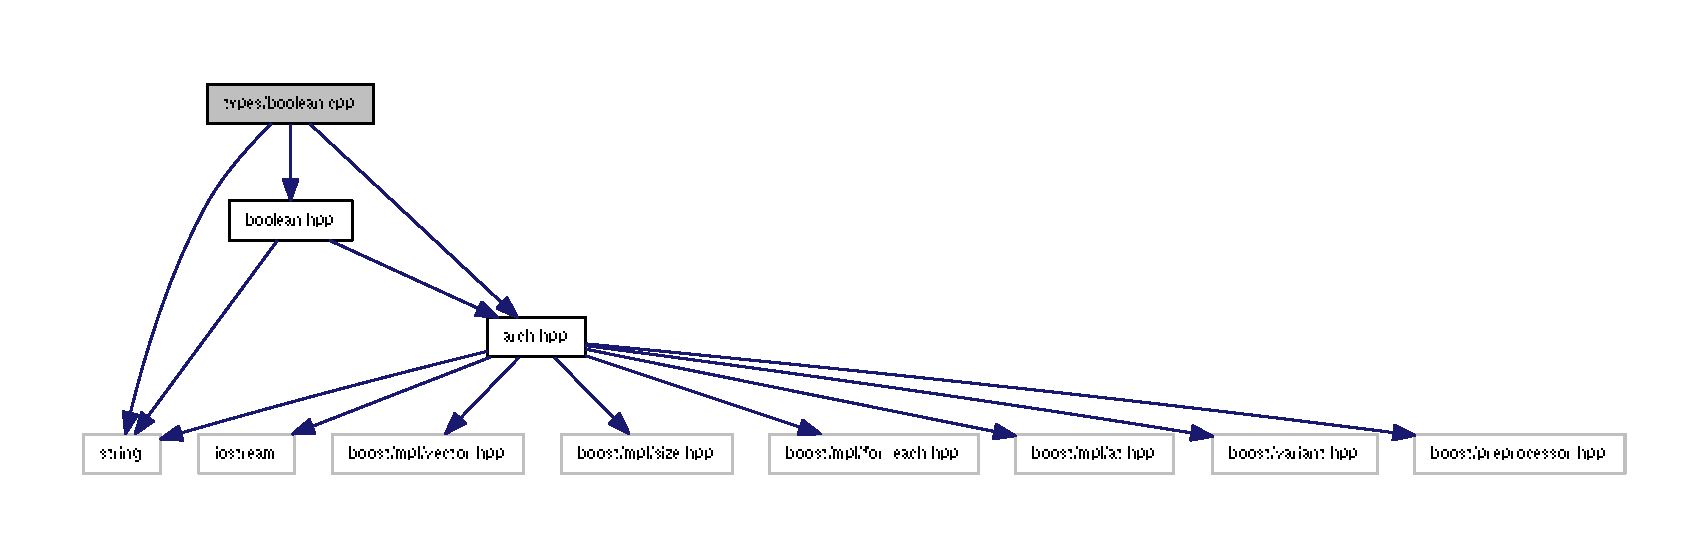
\includegraphics[width=350pt]{boolean_8cpp__incl}
\end{center}
\end{figure}

\hypertarget{boolean_8hpp}{}\section{types/boolean.hpp File Reference}
\label{boolean_8hpp}\index{types/boolean.\+hpp@{types/boolean.\+hpp}}
{\ttfamily \#include \char`\"{}arch.\+hpp\char`\"{}}\\*
{\ttfamily \#include $<$string$>$}\\*
Include dependency graph for boolean.\+hpp\+:
\nopagebreak
\begin{figure}[H]
\begin{center}
\leavevmode
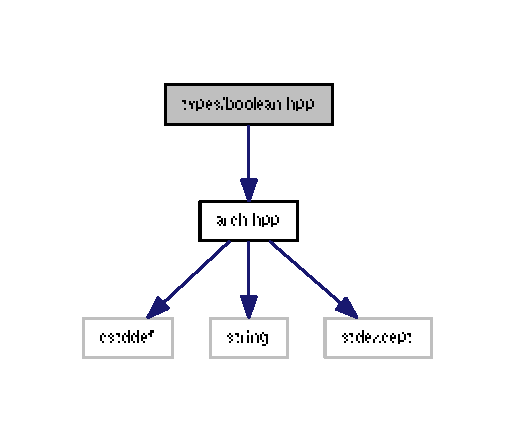
\includegraphics[width=350pt]{boolean_8hpp__incl}
\end{center}
\end{figure}
This graph shows which files directly or indirectly include this file\+:
\nopagebreak
\begin{figure}[H]
\begin{center}
\leavevmode
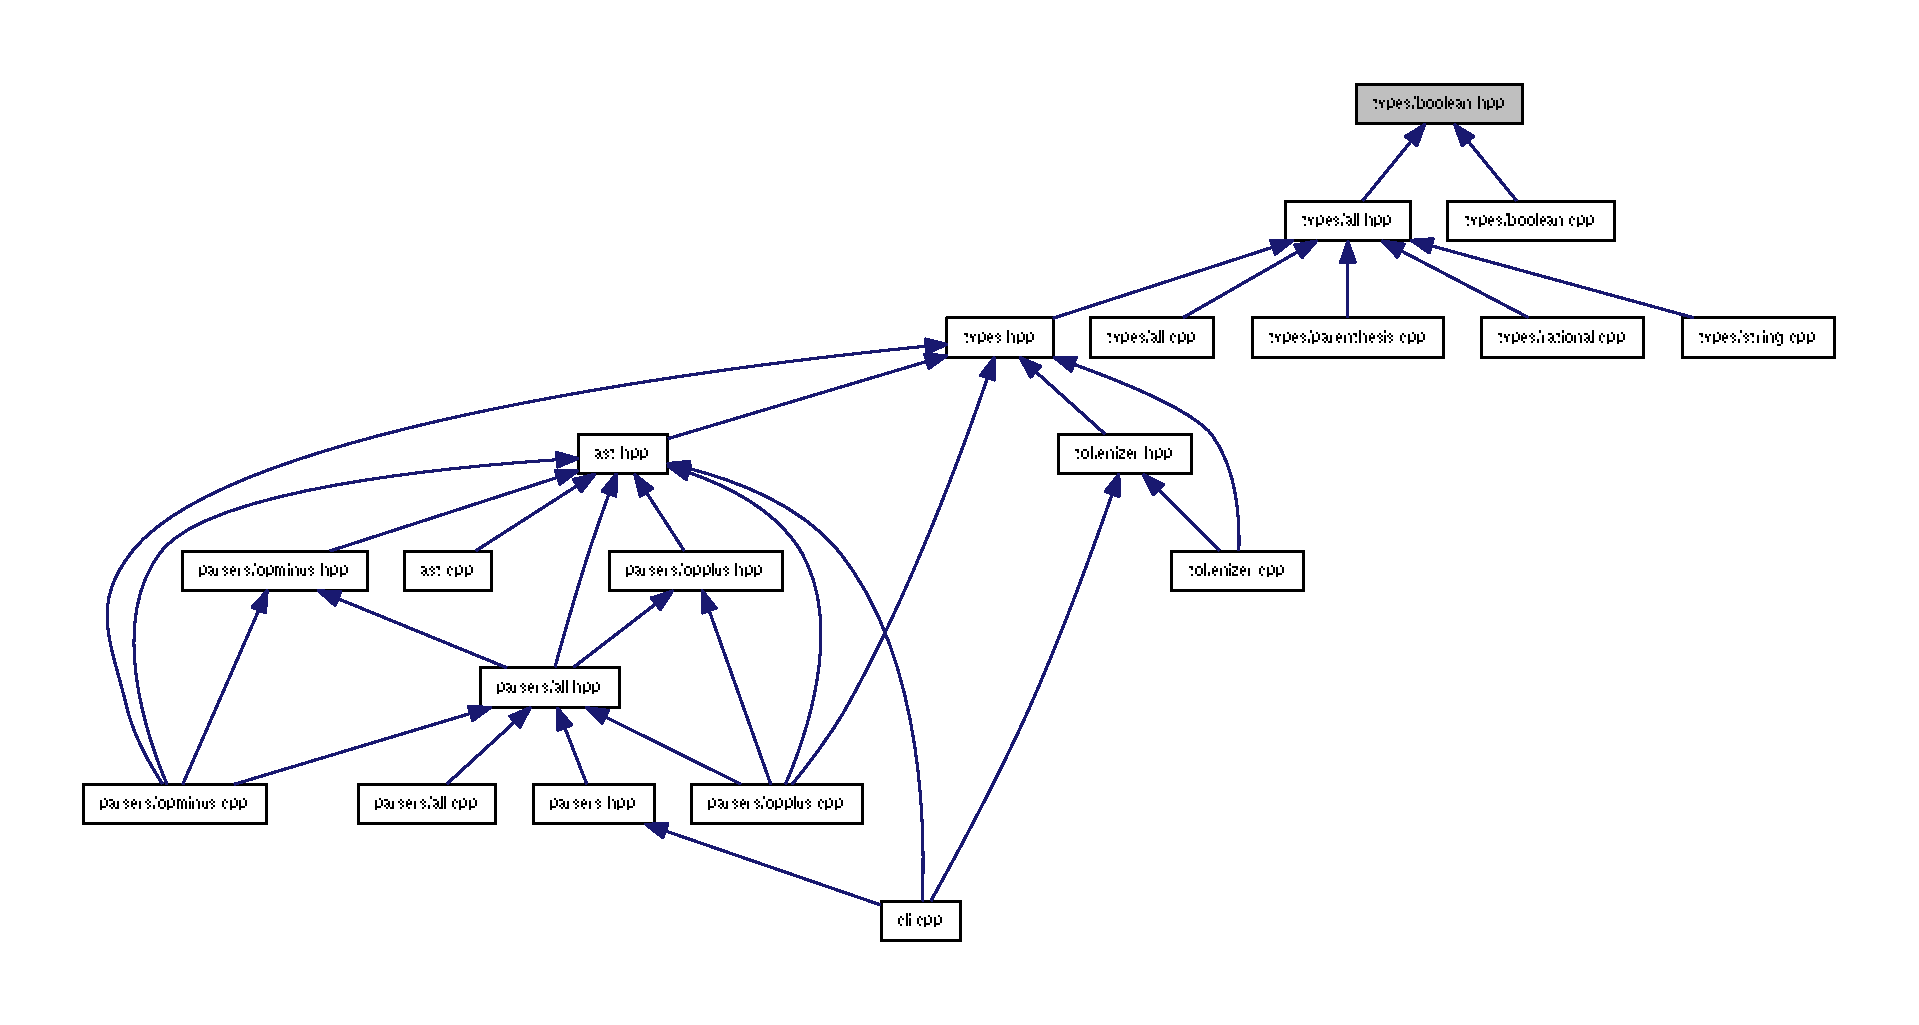
\includegraphics[width=350pt]{boolean_8hpp__dep__incl}
\end{center}
\end{figure}
\subsection*{Typedefs}
\begin{DoxyCompactItemize}
\item 
typedef bool \hyperlink{boolean_8hpp_a0302c79f6d6b93d902af278d1191e054}{Boolean\+Type}
\end{DoxyCompactItemize}


\subsection{Typedef Documentation}
\hypertarget{boolean_8hpp_a0302c79f6d6b93d902af278d1191e054}{}\index{boolean.\+hpp@{boolean.\+hpp}!Boolean\+Type@{Boolean\+Type}}
\index{Boolean\+Type@{Boolean\+Type}!boolean.\+hpp@{boolean.\+hpp}}
\subsubsection[{Boolean\+Type}]{\setlength{\rightskip}{0pt plus 5cm}typedef bool {\bf Boolean\+Type}}\label{boolean_8hpp_a0302c79f6d6b93d902af278d1191e054}


Definition at line 5 of file boolean.\+hpp.


\hypertarget{float_8cpp}{}\section{types/float.cpp File Reference}
\label{float_8cpp}\index{types/float.\+cpp@{types/float.\+cpp}}
{\ttfamily \#include \char`\"{}arch.\+hpp\char`\"{}}\\*
{\ttfamily \#include \char`\"{}float.\+hpp\char`\"{}}\\*
{\ttfamily \#include $<$cstddef$>$}\\*
{\ttfamily \#include $<$string$>$}\\*
{\ttfamily \#include $<$cctype$>$}\\*
{\ttfamily \#include $<$algorithm$>$}\\*
Include dependency graph for float.\+cpp\+:\nopagebreak
\begin{figure}[H]
\begin{center}
\leavevmode
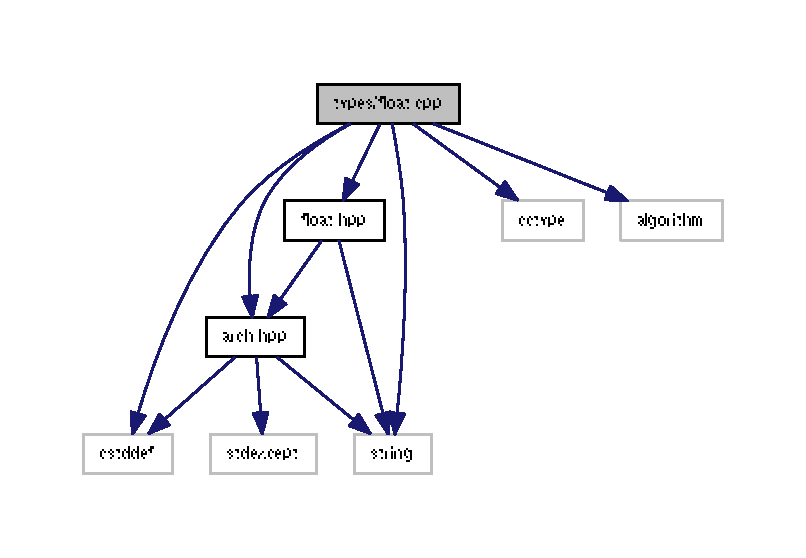
\includegraphics[width=350pt]{float_8cpp__incl}
\end{center}
\end{figure}
\subsection*{Functions}
\begin{DoxyCompactItemize}
\item 
bool \hyperlink{float_8cpp_a2b3841344945adf05970367e441ce957}{is\+Float} (const std\+::string \&token)
\end{DoxyCompactItemize}


\subsection{Function Documentation}
\hypertarget{float_8cpp_a2b3841344945adf05970367e441ce957}{}\index{float.\+cpp@{float.\+cpp}!is\+Float@{is\+Float}}
\index{is\+Float@{is\+Float}!float.\+cpp@{float.\+cpp}}
\subsubsection[{is\+Float}]{\setlength{\rightskip}{0pt plus 5cm}bool is\+Float (
\begin{DoxyParamCaption}
\item[{const std\+::string \&}]{token}
\end{DoxyParamCaption}
)}\label{float_8cpp_a2b3841344945adf05970367e441ce957}


Definition at line 41 of file float.\+cpp.


\hypertarget{float_8hpp}{}\section{types/float.hpp File Reference}
\label{float_8hpp}\index{types/float.\+hpp@{types/float.\+hpp}}
{\ttfamily \#include \char`\"{}arch.\+hpp\char`\"{}}\\*
{\ttfamily \#include $<$string$>$}\\*
Include dependency graph for float.\+hpp\+:\nopagebreak
\begin{figure}[H]
\begin{center}
\leavevmode
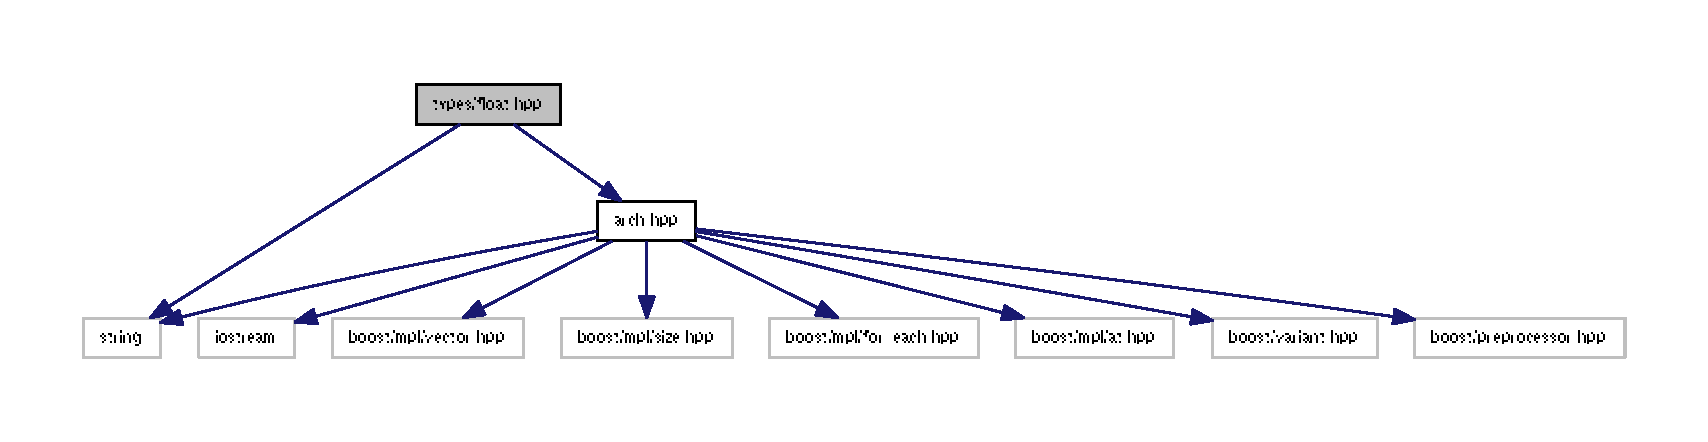
\includegraphics[width=350pt]{float_8hpp__incl}
\end{center}
\end{figure}
This graph shows which files directly or indirectly include this file\+:\nopagebreak
\begin{figure}[H]
\begin{center}
\leavevmode
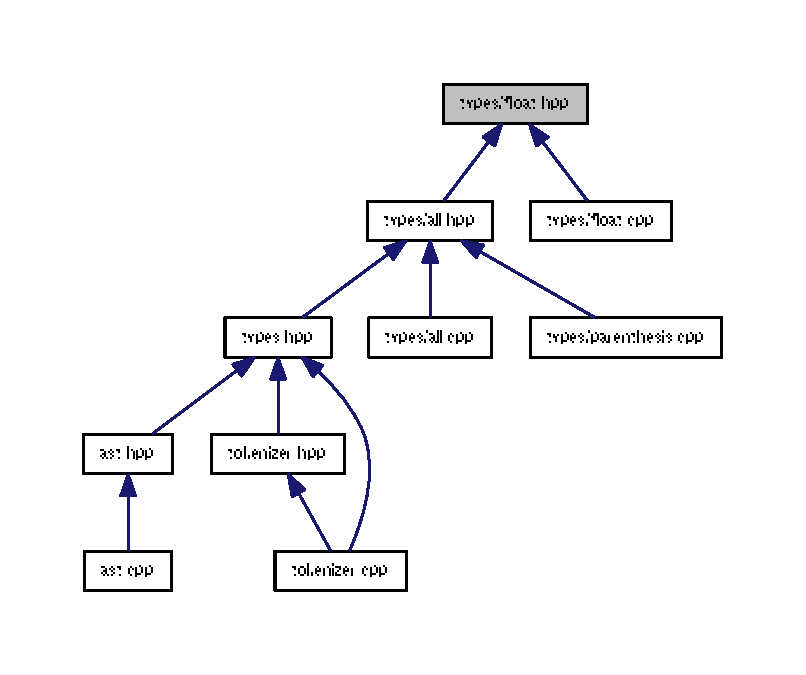
\includegraphics[width=350pt]{float_8hpp__dep__incl}
\end{center}
\end{figure}

\hypertarget{ops_8cpp}{}\section{types/ops.cpp File Reference}
\label{ops_8cpp}\index{types/ops.\+cpp@{types/ops.\+cpp}}
{\ttfamily \#include \char`\"{}arch.\+hpp\char`\"{}}\\*
{\ttfamily \#include \char`\"{}ops.\+hpp\char`\"{}}\\*
{\ttfamily \#include $<$string$>$}\\*
Include dependency graph for ops.\+cpp\+:
\nopagebreak
\begin{figure}[H]
\begin{center}
\leavevmode
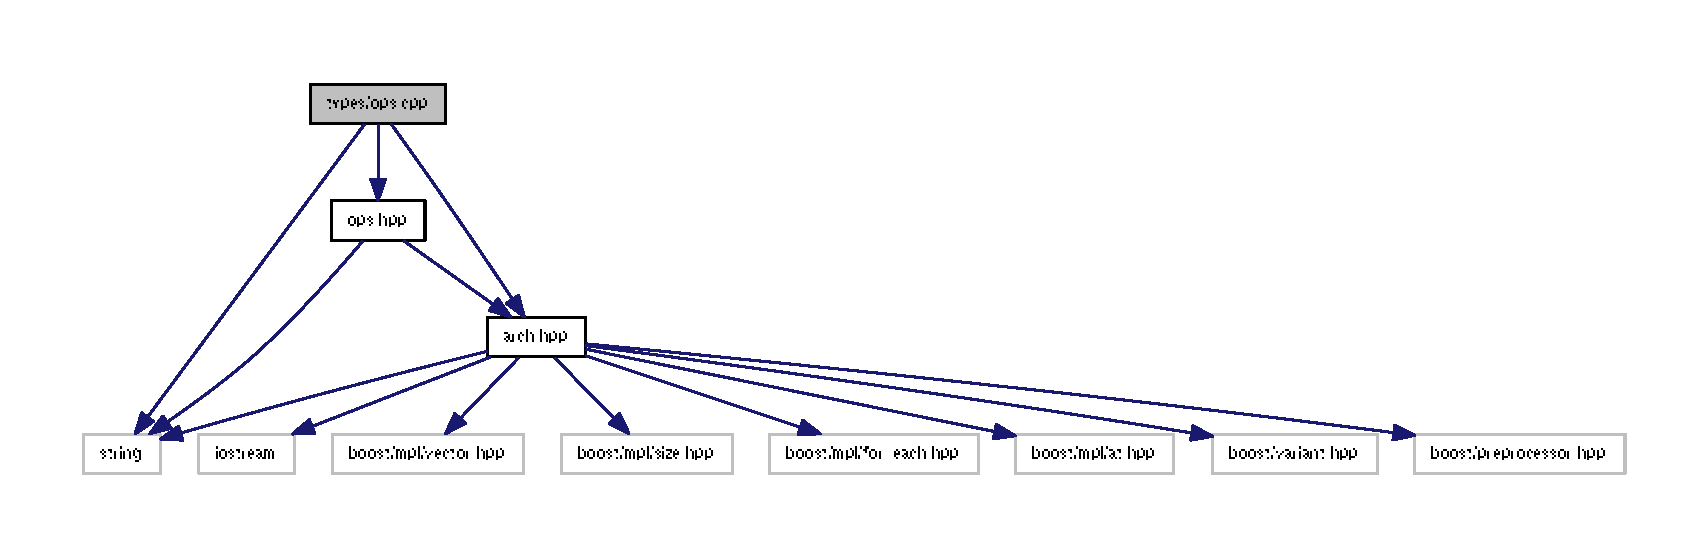
\includegraphics[width=350pt]{ops_8cpp__incl}
\end{center}
\end{figure}

\hypertarget{ops_8hpp}{}\section{types/ops.hpp File Reference}
\label{ops_8hpp}\index{types/ops.\+hpp@{types/ops.\+hpp}}
{\ttfamily \#include $<$string$>$}\\*
{\ttfamily \#include \char`\"{}arch.\+hpp\char`\"{}}\\*
Include dependency graph for ops.\+hpp\+:\nopagebreak
\begin{figure}[H]
\begin{center}
\leavevmode
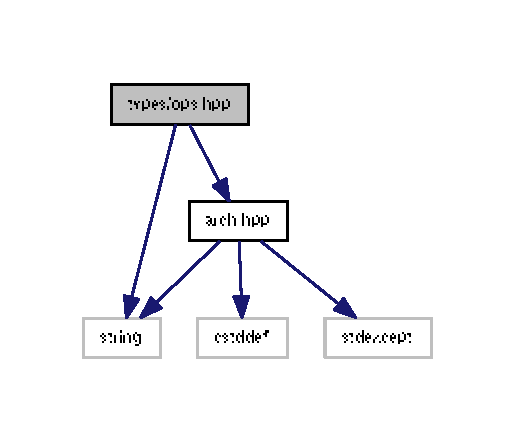
\includegraphics[width=350pt]{ops_8hpp__incl}
\end{center}
\end{figure}
This graph shows which files directly or indirectly include this file\+:\nopagebreak
\begin{figure}[H]
\begin{center}
\leavevmode
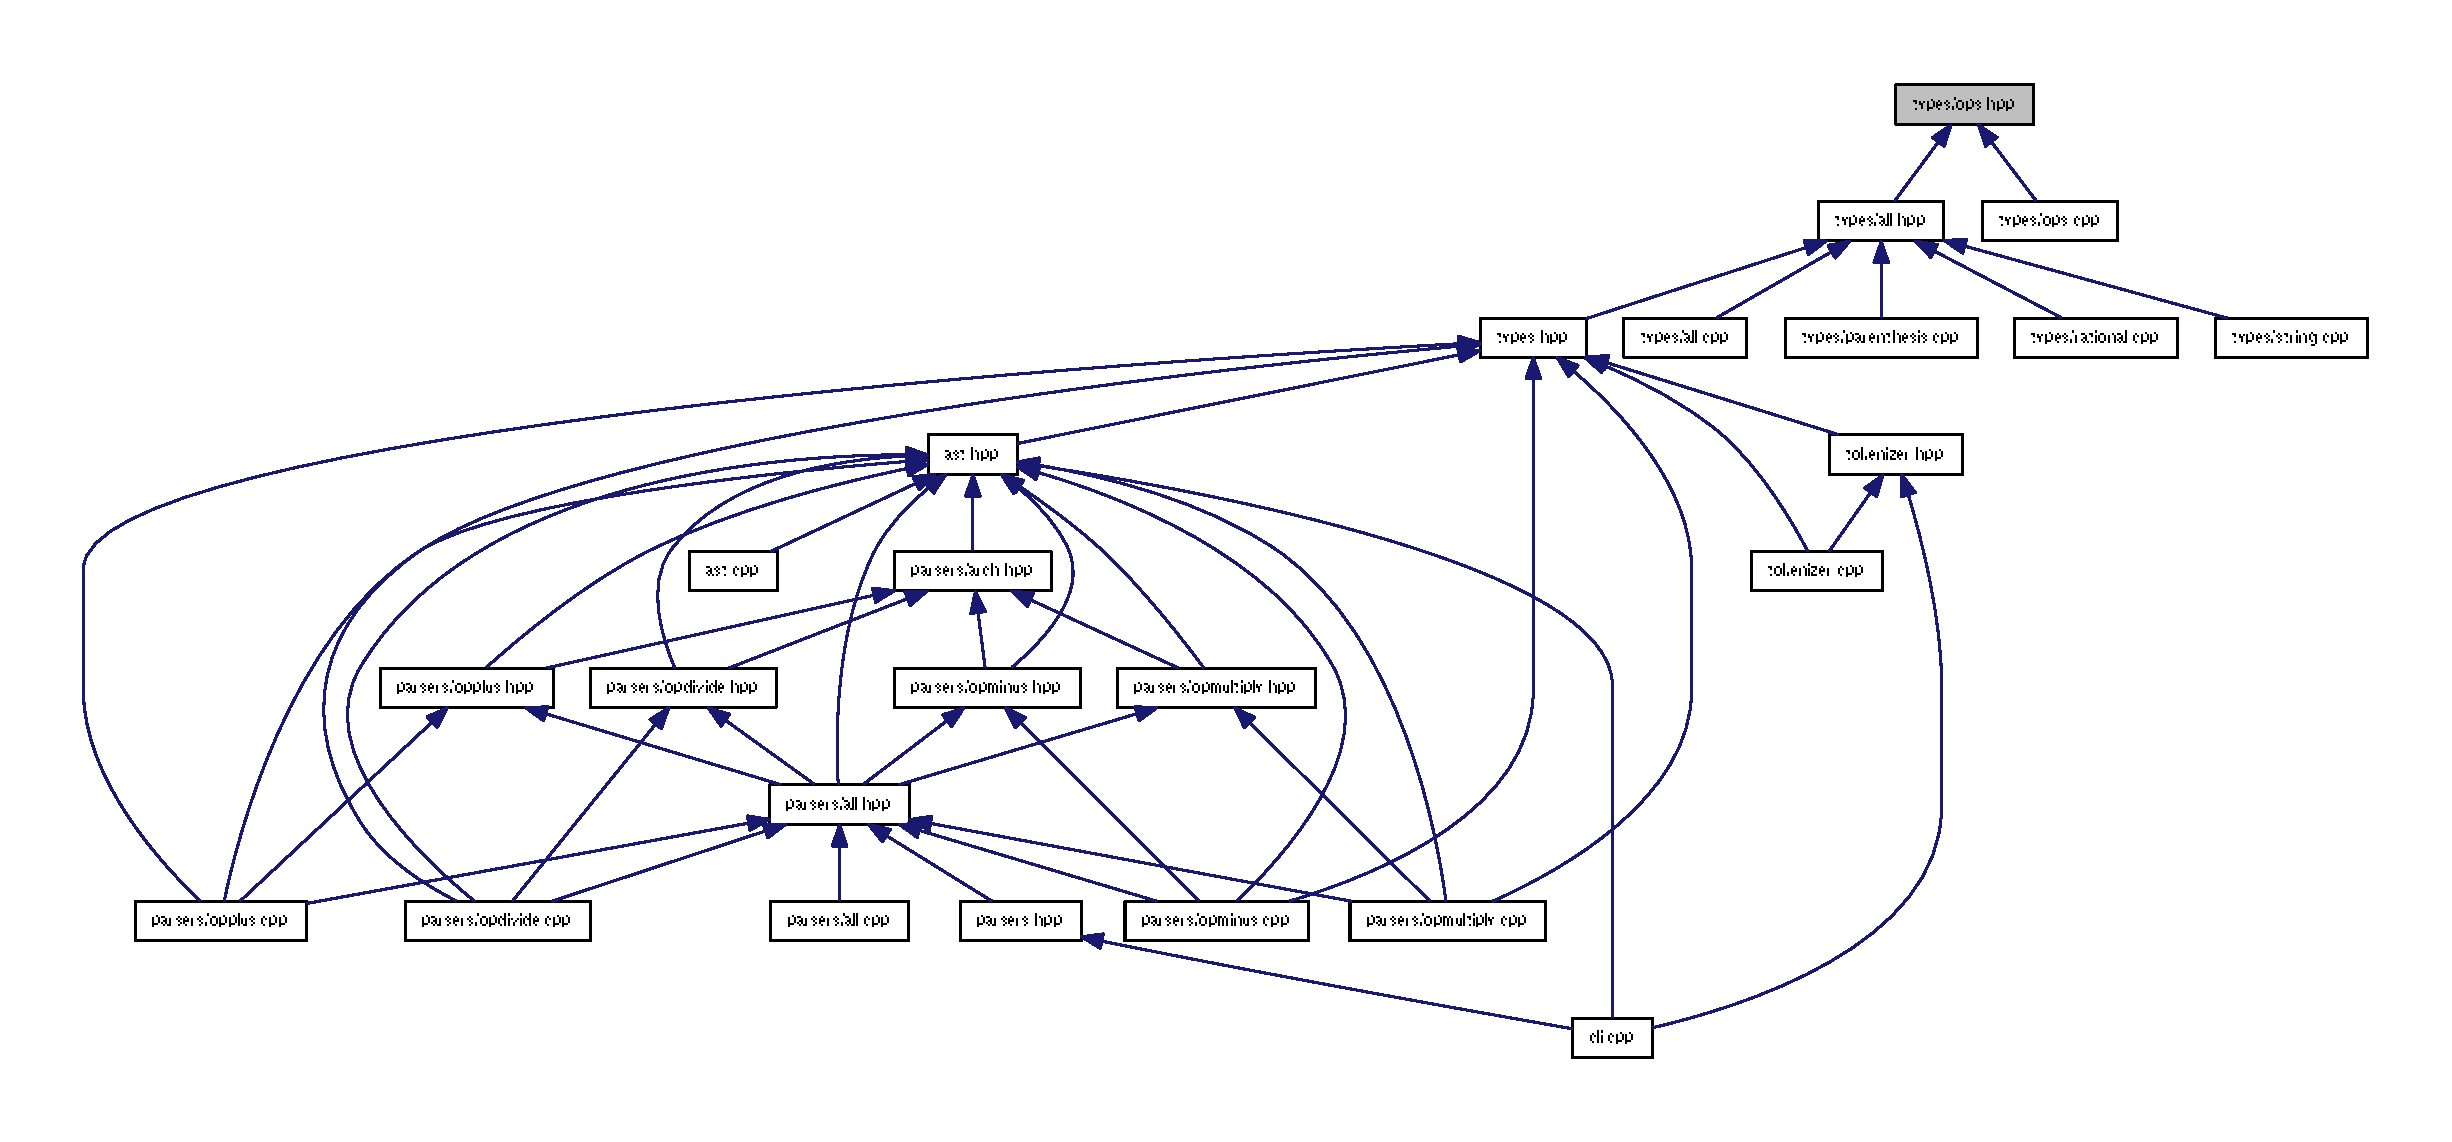
\includegraphics[width=350pt]{ops_8hpp__dep__incl}
\end{center}
\end{figure}

\hypertarget{parenthesis_8cpp}{}\section{types/parenthesis.cpp File Reference}
\label{parenthesis_8cpp}\index{types/parenthesis.\+cpp@{types/parenthesis.\+cpp}}
{\ttfamily \#include \char`\"{}all.\+hpp\char`\"{}}\\*
{\ttfamily \#include \char`\"{}parenthesis.\+hpp\char`\"{}}\\*
Include dependency graph for parenthesis.\+cpp\+:
\nopagebreak
\begin{figure}[H]
\begin{center}
\leavevmode
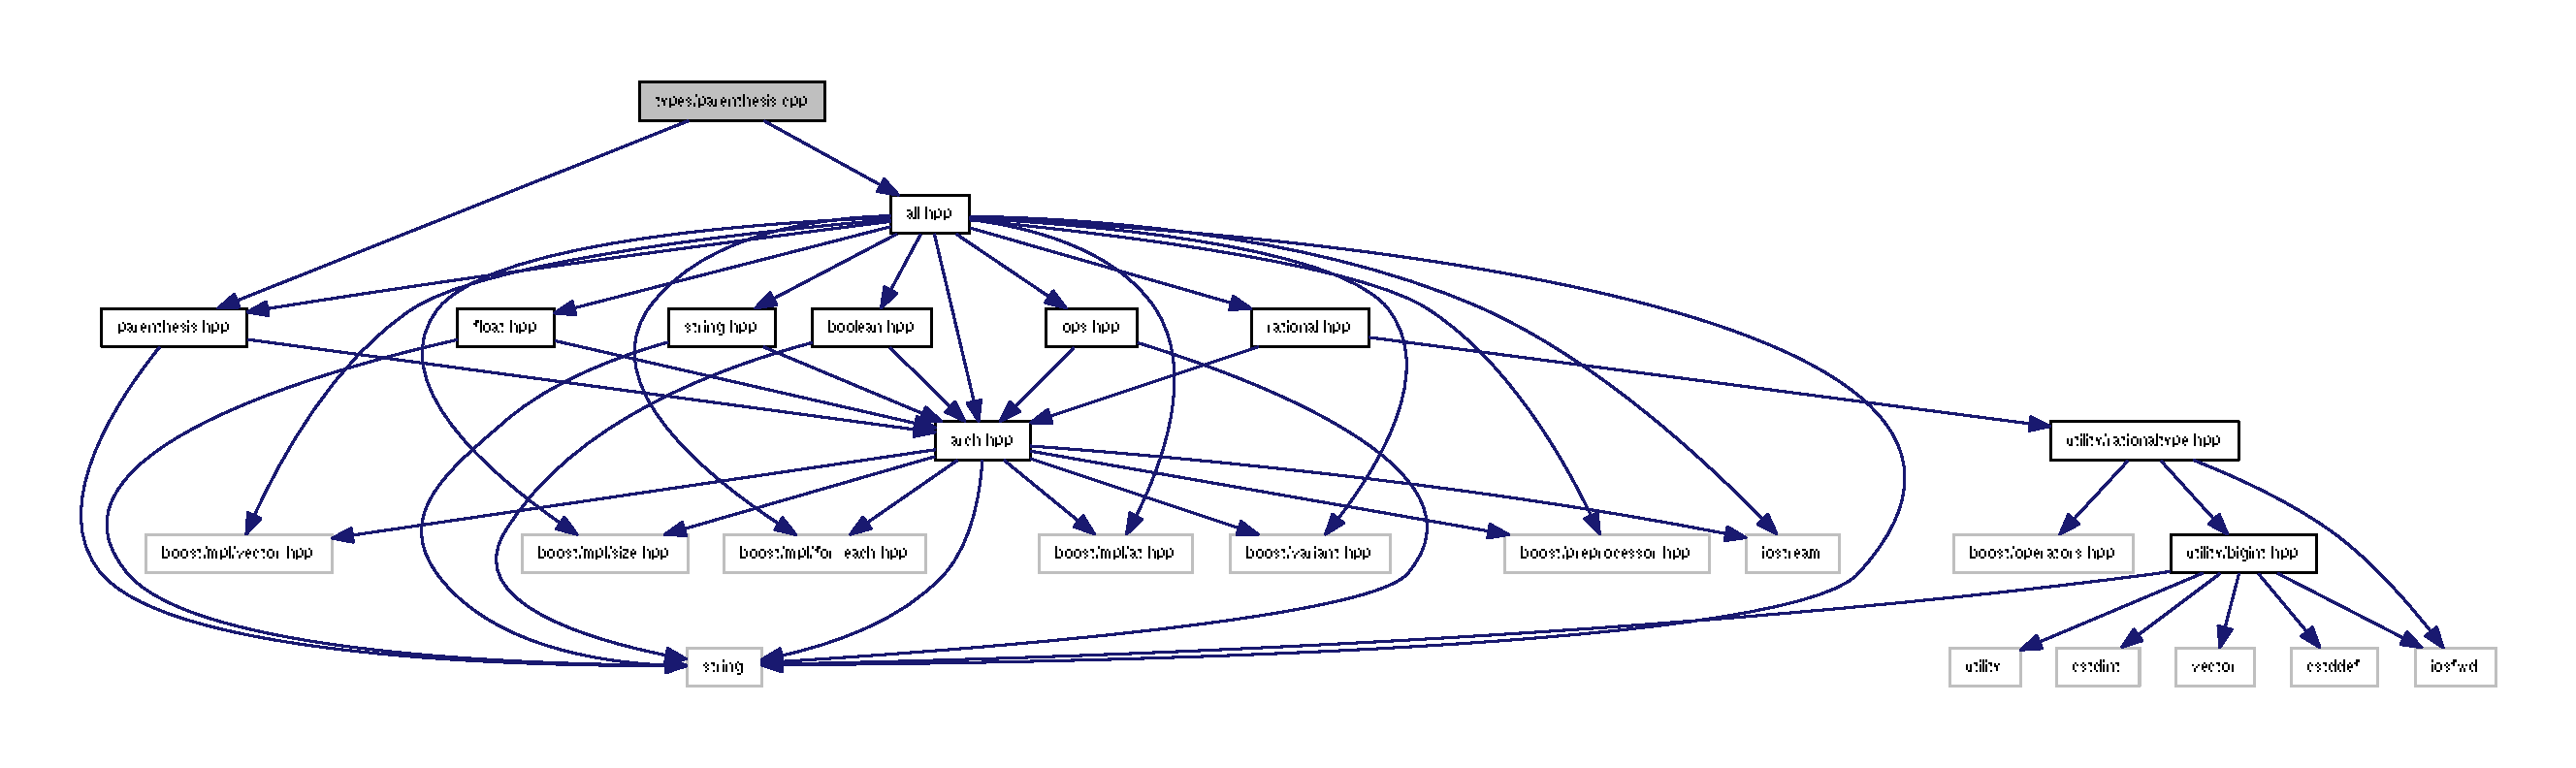
\includegraphics[width=350pt]{parenthesis_8cpp__incl}
\end{center}
\end{figure}

\hypertarget{parenthesis_8hpp}{}\section{types/parenthesis.hpp File Reference}
\label{parenthesis_8hpp}\index{types/parenthesis.\+hpp@{types/parenthesis.\+hpp}}
{\ttfamily \#include \char`\"{}arch.\+hpp\char`\"{}}\\*
{\ttfamily \#include $<$string$>$}\\*
Include dependency graph for parenthesis.\+hpp\+:
\nopagebreak
\begin{figure}[H]
\begin{center}
\leavevmode
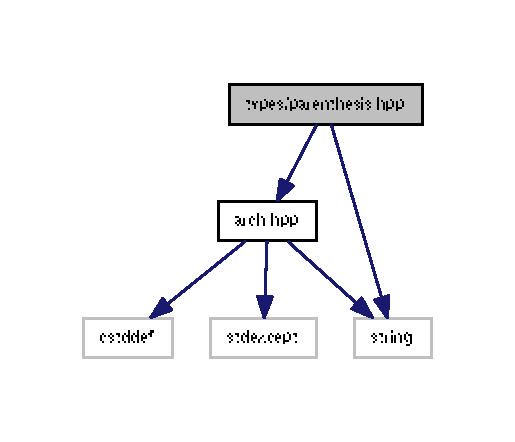
\includegraphics[width=350pt]{parenthesis_8hpp__incl}
\end{center}
\end{figure}
This graph shows which files directly or indirectly include this file\+:
\nopagebreak
\begin{figure}[H]
\begin{center}
\leavevmode
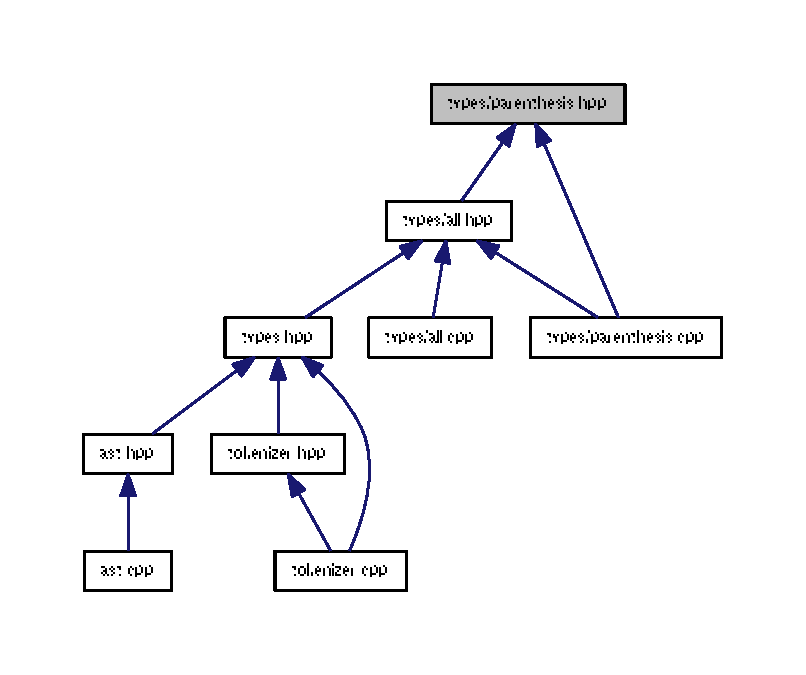
\includegraphics[width=350pt]{parenthesis_8hpp__dep__incl}
\end{center}
\end{figure}

\hypertarget{rational_8cpp}{}\section{types/rational.cpp File Reference}
\label{rational_8cpp}\index{types/rational.\+cpp@{types/rational.\+cpp}}
{\ttfamily \#include \char`\"{}rational.\+hpp\char`\"{}}\\*
{\ttfamily \#include \char`\"{}all.\+hpp\char`\"{}}\\*
{\ttfamily \#include \char`\"{}utility/simplenum.\+hpp\char`\"{}}\\*
{\ttfamily \#include $<$sstream$>$}\\*
Include dependency graph for rational.\+cpp\+:\nopagebreak
\begin{figure}[H]
\begin{center}
\leavevmode
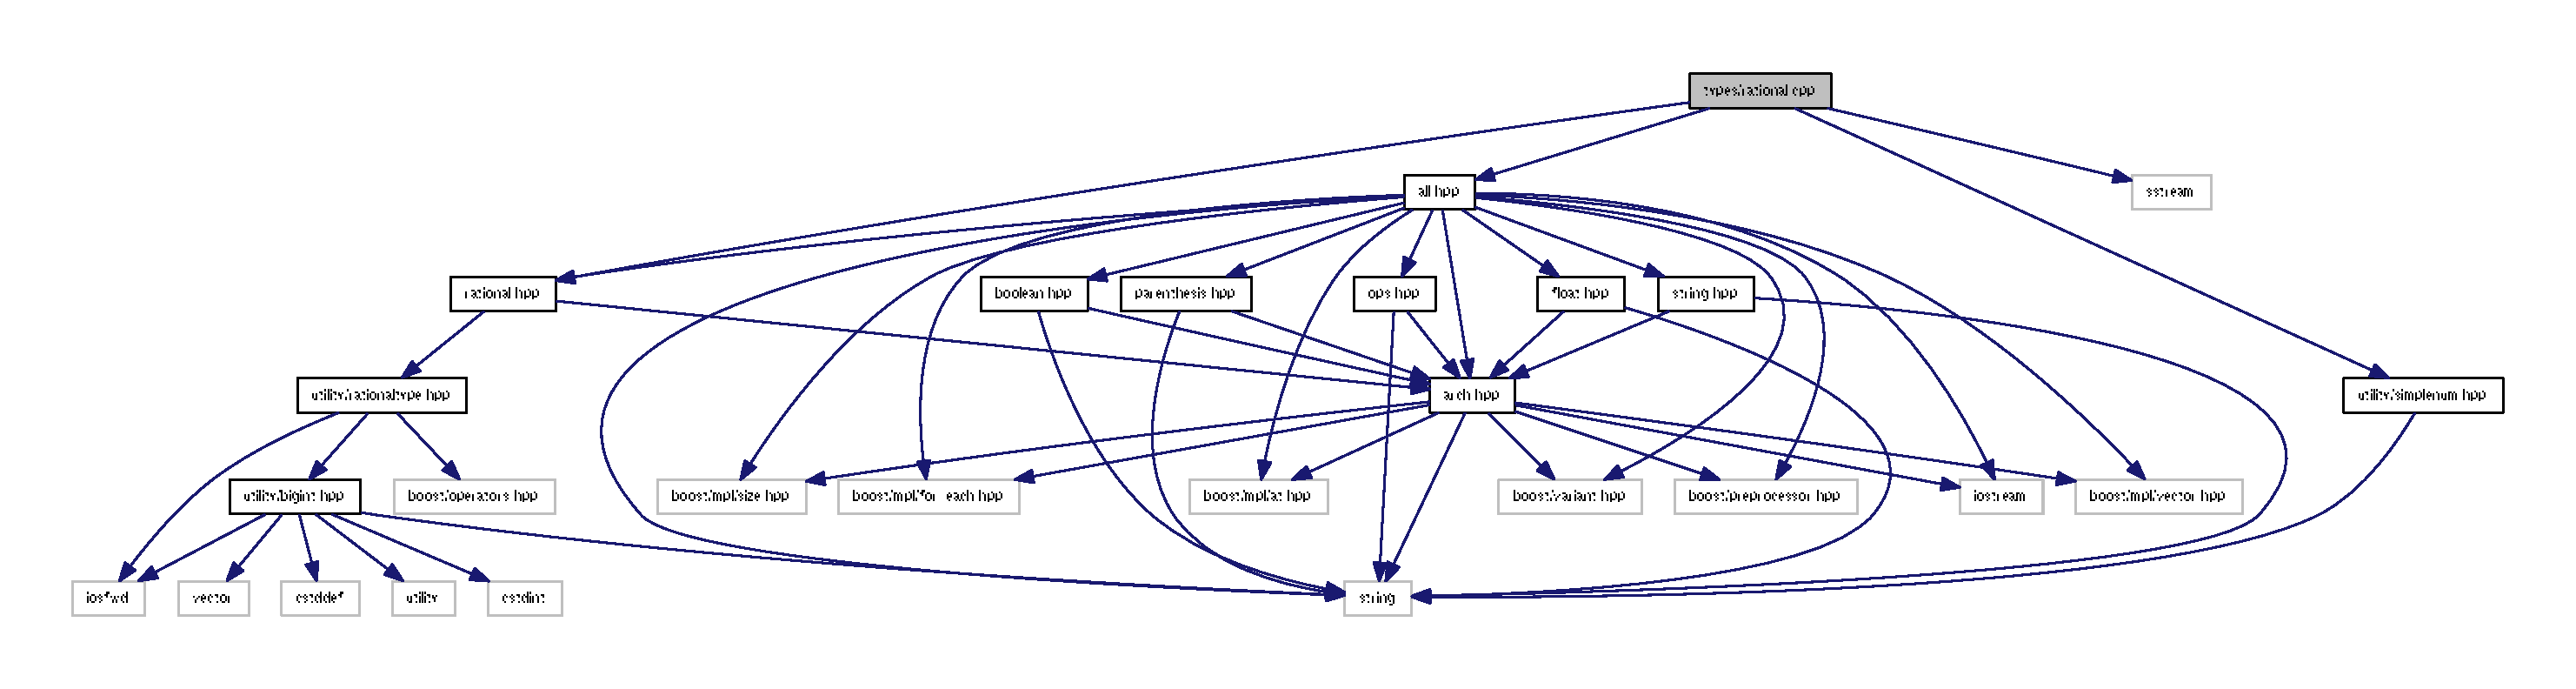
\includegraphics[width=350pt]{rational_8cpp__incl}
\end{center}
\end{figure}

\hypertarget{rational_8hpp}{}\section{types/rational.hpp File Reference}
\label{rational_8hpp}\index{types/rational.\+hpp@{types/rational.\+hpp}}
{\ttfamily \#include \char`\"{}arch.\+hpp\char`\"{}}\\*
{\ttfamily \#include \char`\"{}utility/bigint.\+hpp\char`\"{}}\\*
Include dependency graph for rational.\+hpp\+:\nopagebreak
\begin{figure}[H]
\begin{center}
\leavevmode
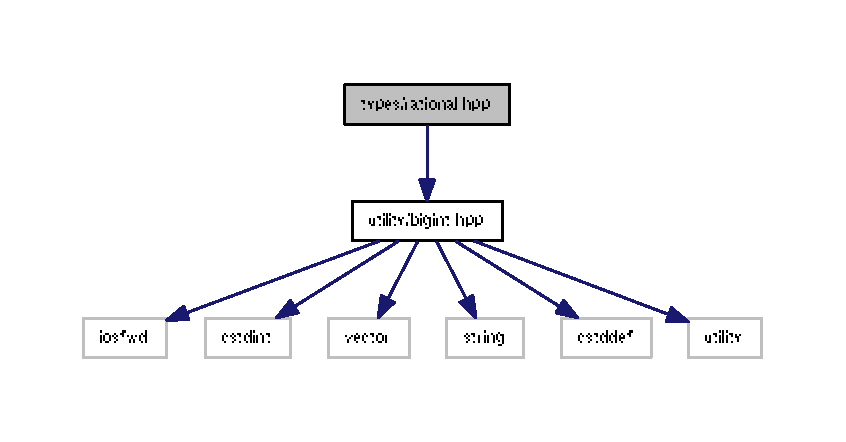
\includegraphics[width=350pt]{rational_8hpp__incl}
\end{center}
\end{figure}
This graph shows which files directly or indirectly include this file\+:\nopagebreak
\begin{figure}[H]
\begin{center}
\leavevmode
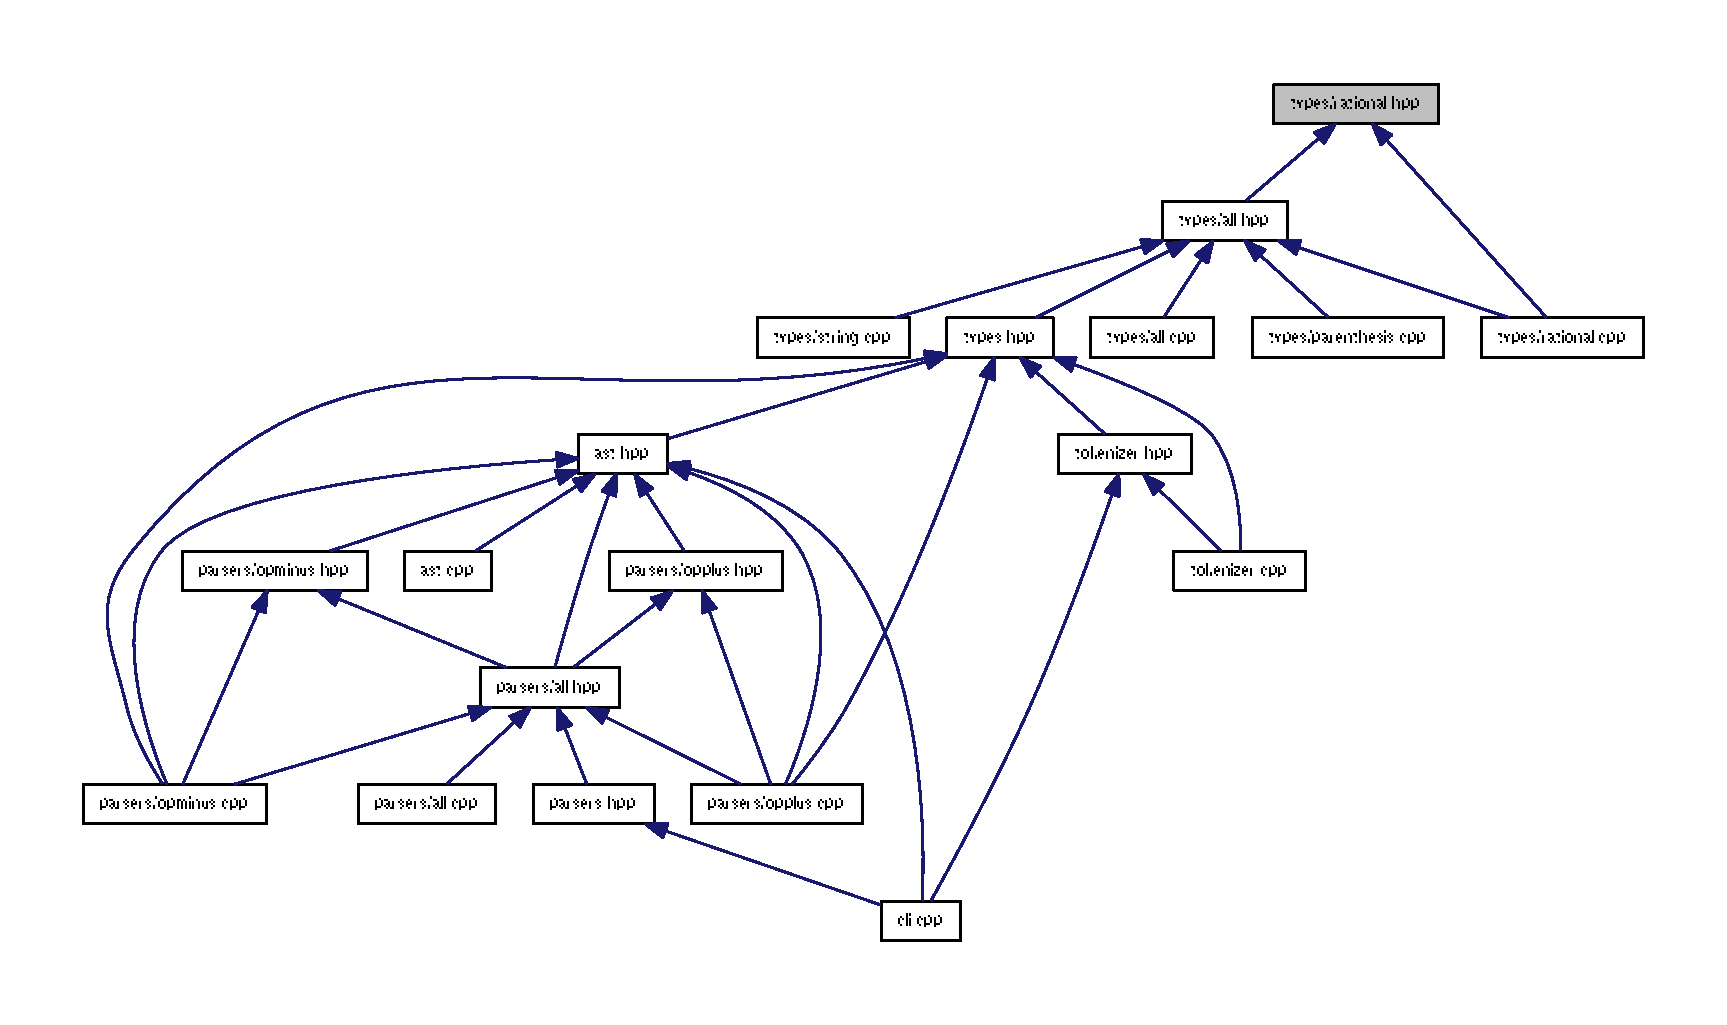
\includegraphics[width=350pt]{rational_8hpp__dep__incl}
\end{center}
\end{figure}
\subsection*{Classes}
\begin{DoxyCompactItemize}
\item 
class \hyperlink{class_rational_type}{Rational\+Type}
\end{DoxyCompactItemize}

\hypertarget{string_8cpp}{}\section{types/string.cpp File Reference}
\label{string_8cpp}\index{types/string.\+cpp@{types/string.\+cpp}}
{\ttfamily \#include \char`\"{}string.\+hpp\char`\"{}}\\*
{\ttfamily \#include \char`\"{}all.\+hpp\char`\"{}}\\*
{\ttfamily \#include \char`\"{}utility/strutility.\+hpp\char`\"{}}\\*
{\ttfamily \#include $<$string$>$}\\*
Include dependency graph for string.\+cpp\+:\nopagebreak
\begin{figure}[H]
\begin{center}
\leavevmode
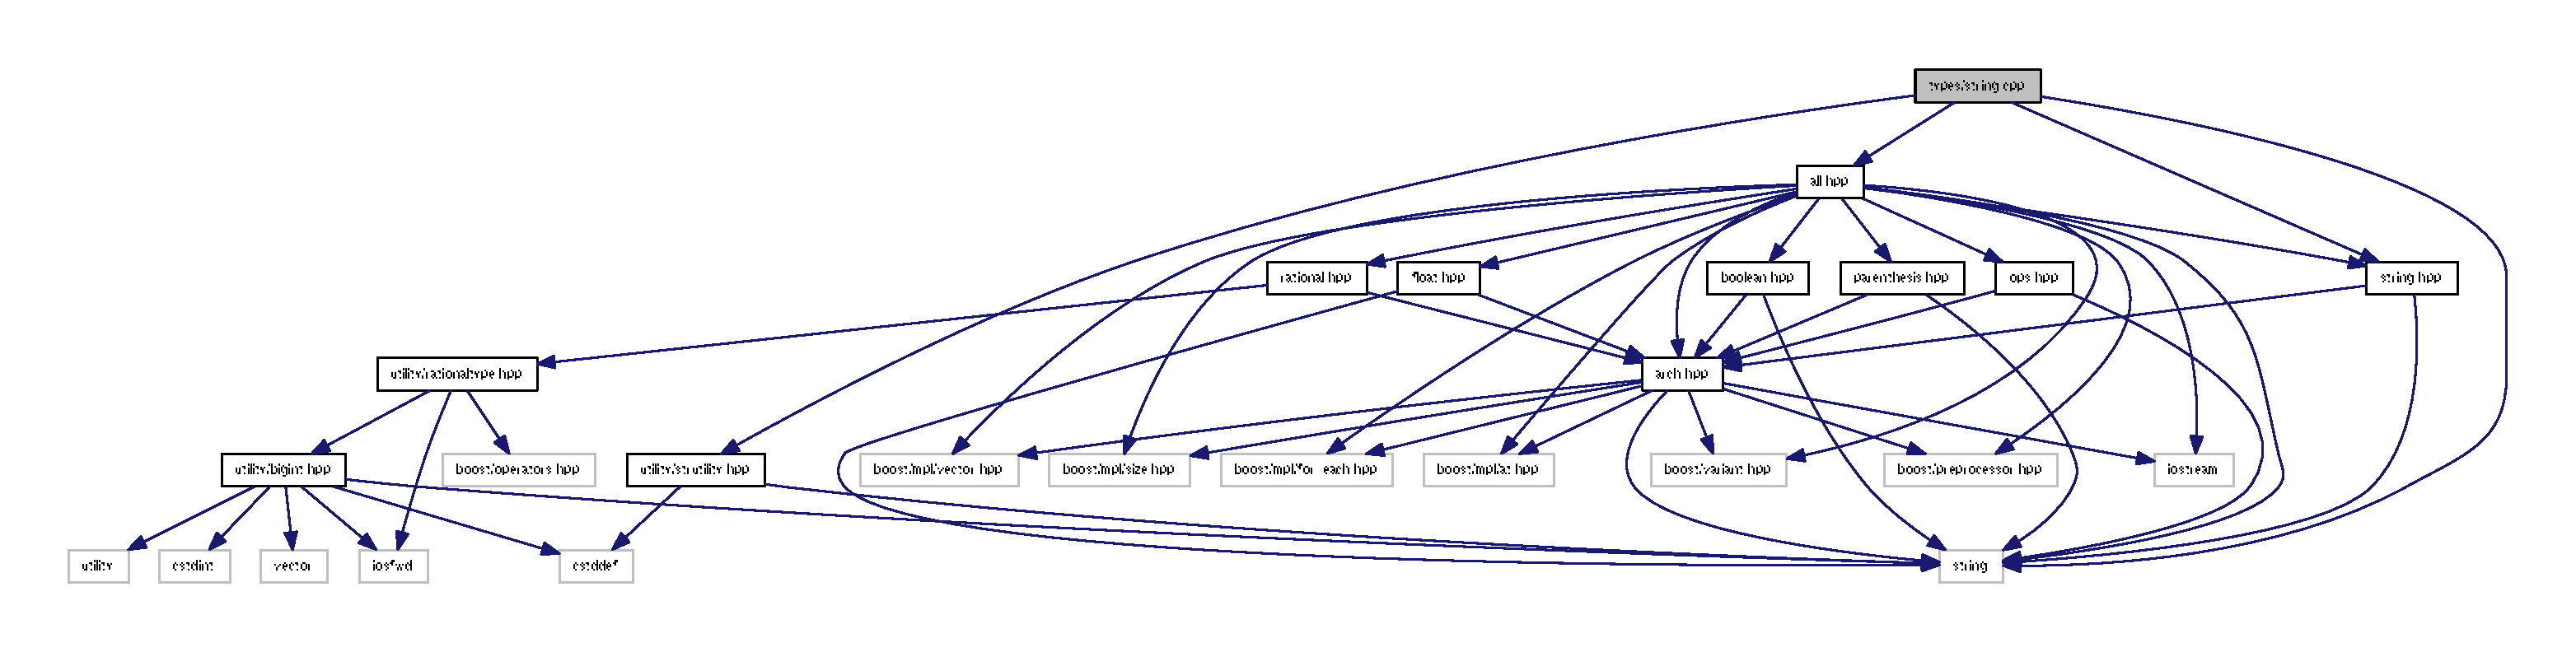
\includegraphics[width=350pt]{string_8cpp__incl}
\end{center}
\end{figure}

\hypertarget{string_8hpp}{}\section{types/string.hpp File Reference}
\label{string_8hpp}\index{types/string.\+hpp@{types/string.\+hpp}}
{\ttfamily \#include \char`\"{}arch.\+hpp\char`\"{}}\\*
{\ttfamily \#include $<$string$>$}\\*
Include dependency graph for string.\+hpp\+:\nopagebreak
\begin{figure}[H]
\begin{center}
\leavevmode
\includegraphics[width=350pt]{string_8hpp__incl}
\end{center}
\end{figure}
This graph shows which files directly or indirectly include this file\+:
\nopagebreak
\begin{figure}[H]
\begin{center}
\leavevmode
\includegraphics[width=350pt]{string_8hpp__dep__incl}
\end{center}
\end{figure}

\hypertarget{bigint_8cpp}{}\section{utility/bigint.cpp File Reference}
\label{bigint_8cpp}\index{utility/bigint.\+cpp@{utility/bigint.\+cpp}}
{\ttfamily \#include $<$iostream$>$}\\*
{\ttfamily \#include $<$cstdint$>$}\\*
{\ttfamily \#include $<$cstddef$>$}\\*
{\ttfamily \#include $<$vector$>$}\\*
{\ttfamily \#include $<$string$>$}\\*
{\ttfamily \#include $<$cmath$>$}\\*
{\ttfamily \#include $<$cctype$>$}\\*
{\ttfamily \#include $<$stdexcept$>$}\\*
{\ttfamily \#include $<$cassert$>$}\\*
{\ttfamily \#include $<$algorithm$>$}\\*
{\ttfamily \#include $<$utility$>$}\\*
{\ttfamily \#include $<$functional$>$}\\*
{\ttfamily \#include \char`\"{}bigint.\+hpp\char`\"{}}\\*
{\ttfamily \#include \char`\"{}utility/strutility.\+hpp\char`\"{}}\\*
Include dependency graph for bigint.\+cpp\+:\nopagebreak
\begin{figure}[H]
\begin{center}
\leavevmode
\includegraphics[width=350pt]{bigint_8cpp__incl}
\end{center}
\end{figure}
\subsection*{Functions}
\begin{DoxyCompactItemize}
\item 
{\footnotesize template$<$typename Compare\+Func $>$ }\\bool \hyperlink{bigint_8cpp_a95ccae99f465fac11bf28196f62dac03}{raw\+Compare} (const \hyperlink{class_big_int}{Big\+Int} \&a, const \hyperlink{class_big_int}{Big\+Int} \&b)
\item 
std\+::istream \& \hyperlink{bigint_8cpp_abfb3d978331870b4cba82ece17354f44}{operator$>$$>$} (std\+::istream \&i, \hyperlink{class_big_int}{Big\+Int} \&b)
\item 
std\+::ostream \& \hyperlink{bigint_8cpp_a0d8814d1177634c5e0ee08e2bbccf328}{operator$<$$<$} (std\+::ostream \&o, const \hyperlink{class_big_int}{Big\+Int} \&b)
\end{DoxyCompactItemize}


\subsection{Function Documentation}
\hypertarget{bigint_8cpp_a0d8814d1177634c5e0ee08e2bbccf328}{}\index{bigint.\+cpp@{bigint.\+cpp}!operator$<$$<$@{operator$<$$<$}}
\index{operator$<$$<$@{operator$<$$<$}!bigint.\+cpp@{bigint.\+cpp}}
\subsubsection[{operator$<$$<$}]{\setlength{\rightskip}{0pt plus 5cm}std\+::ostream\& operator$<$$<$ (
\begin{DoxyParamCaption}
\item[{std\+::ostream \&}]{o, }
\item[{const {\bf Big\+Int} \&}]{b}
\end{DoxyParamCaption}
)}\label{bigint_8cpp_a0d8814d1177634c5e0ee08e2bbccf328}


Definition at line 248 of file bigint.\+cpp.

\hypertarget{bigint_8cpp_abfb3d978331870b4cba82ece17354f44}{}\index{bigint.\+cpp@{bigint.\+cpp}!operator$>$$>$@{operator$>$$>$}}
\index{operator$>$$>$@{operator$>$$>$}!bigint.\+cpp@{bigint.\+cpp}}
\subsubsection[{operator$>$$>$}]{\setlength{\rightskip}{0pt plus 5cm}std\+::istream\& operator$>$$>$ (
\begin{DoxyParamCaption}
\item[{std\+::istream \&}]{i, }
\item[{{\bf Big\+Int} \&}]{b}
\end{DoxyParamCaption}
)}\label{bigint_8cpp_abfb3d978331870b4cba82ece17354f44}


Definition at line 240 of file bigint.\+cpp.

\hypertarget{bigint_8cpp_a95ccae99f465fac11bf28196f62dac03}{}\index{bigint.\+cpp@{bigint.\+cpp}!raw\+Compare@{raw\+Compare}}
\index{raw\+Compare@{raw\+Compare}!bigint.\+cpp@{bigint.\+cpp}}
\subsubsection[{raw\+Compare}]{\setlength{\rightskip}{0pt plus 5cm}template$<$typename Compare\+Func $>$ bool raw\+Compare (
\begin{DoxyParamCaption}
\item[{const {\bf Big\+Int} \&}]{a, }
\item[{const {\bf Big\+Int} \&}]{b}
\end{DoxyParamCaption}
)}\label{bigint_8cpp_a95ccae99f465fac11bf28196f62dac03}


Definition at line 104 of file bigint.\+cpp.


\hypertarget{bigint_8hpp}{}\section{utility/bigint.hpp File Reference}
\label{bigint_8hpp}\index{utility/bigint.\+hpp@{utility/bigint.\+hpp}}
{\ttfamily \#include $<$iosfwd$>$}\\*
{\ttfamily \#include $<$cstdint$>$}\\*
{\ttfamily \#include $<$vector$>$}\\*
{\ttfamily \#include $<$string$>$}\\*
{\ttfamily \#include $<$cstddef$>$}\\*
Include dependency graph for bigint.\+hpp\+:
% FIG 0
This graph shows which files directly or indirectly include this file\+:
% FIG 1
\subsection*{Classes}
\begin{DoxyCompactItemize}
\item 
class \hyperlink{class_big_int}{Big\+Int}
\end{DoxyCompactItemize}

\hypertarget{rationaltype_8cpp}{}\section{utility/rationaltype.cpp File Reference}
\label{rationaltype_8cpp}\index{utility/rationaltype.\+cpp@{utility/rationaltype.\+cpp}}
{\ttfamily \#include \char`\"{}rationaltype.\+hpp\char`\"{}}\\*
{\ttfamily \#include \char`\"{}utility/bigint.\+hpp\char`\"{}}\\*
{\ttfamily \#include $<$stdexcept$>$}\\*
{\ttfamily \#include $<$iostream$>$}\\*
{\ttfamily \#include $<$string$>$}\\*
Include dependency graph for rationaltype.\+cpp\+:
\nopagebreak
\begin{figure}[H]
\begin{center}
\leavevmode
\includegraphics[width=350pt]{rationaltype_8cpp__incl}
\end{center}
\end{figure}
\subsection*{Functions}
\begin{DoxyCompactItemize}
\item 
std\+::istream \& \hyperlink{rationaltype_8cpp_a03ba623b12ad5e6e6df81ba8fad47981}{operator$>$$>$} (std\+::istream \&i, \hyperlink{class_rational_type}{Rational\+Type} \&a)
\item 
std\+::ostream \& \hyperlink{rationaltype_8cpp_ad1e553a2da4313b37b5bf59bdeb16655}{operator$<$$<$} (std\+::ostream \&o, const \hyperlink{class_rational_type}{Rational\+Type} \&a)
\end{DoxyCompactItemize}


\subsection{Function Documentation}
\hypertarget{rationaltype_8cpp_ad1e553a2da4313b37b5bf59bdeb16655}{}\index{rationaltype.\+cpp@{rationaltype.\+cpp}!operator$<$$<$@{operator$<$$<$}}
\index{operator$<$$<$@{operator$<$$<$}!rationaltype.\+cpp@{rationaltype.\+cpp}}
\subsubsection[{operator$<$$<$}]{\setlength{\rightskip}{0pt plus 5cm}std\+::ostream\& operator$<$$<$ (
\begin{DoxyParamCaption}
\item[{std\+::ostream \&}]{o, }
\item[{const {\bf Rational\+Type} \&}]{a}
\end{DoxyParamCaption}
)}\label{rationaltype_8cpp_ad1e553a2da4313b37b5bf59bdeb16655}


Definition at line 91 of file rationaltype.\+cpp.

\hypertarget{rationaltype_8cpp_a03ba623b12ad5e6e6df81ba8fad47981}{}\index{rationaltype.\+cpp@{rationaltype.\+cpp}!operator$>$$>$@{operator$>$$>$}}
\index{operator$>$$>$@{operator$>$$>$}!rationaltype.\+cpp@{rationaltype.\+cpp}}
\subsubsection[{operator$>$$>$}]{\setlength{\rightskip}{0pt plus 5cm}std\+::istream\& operator$>$$>$ (
\begin{DoxyParamCaption}
\item[{std\+::istream \&}]{i, }
\item[{{\bf Rational\+Type} \&}]{a}
\end{DoxyParamCaption}
)}\label{rationaltype_8cpp_a03ba623b12ad5e6e6df81ba8fad47981}


Definition at line 80 of file rationaltype.\+cpp.


\hypertarget{rationaltype_8hpp}{}\section{utility/rationaltype.hpp File Reference}
\label{rationaltype_8hpp}\index{utility/rationaltype.\+hpp@{utility/rationaltype.\+hpp}}
{\ttfamily \#include \char`\"{}utility/bigint.\+hpp\char`\"{}}\\*
{\ttfamily \#include $<$boost/operators.\+hpp$>$}\\*
{\ttfamily \#include $<$iosfwd$>$}\\*
Include dependency graph for rationaltype.\+hpp\+:\nopagebreak
\begin{figure}[H]
\begin{center}
\leavevmode
\includegraphics[width=350pt]{rationaltype_8hpp__incl}
\end{center}
\end{figure}
This graph shows which files directly or indirectly include this file\+:
\nopagebreak
\begin{figure}[H]
\begin{center}
\leavevmode
\includegraphics[width=350pt]{rationaltype_8hpp__dep__incl}
\end{center}
\end{figure}
\subsection*{Classes}
\begin{DoxyCompactItemize}
\item 
class \hyperlink{class_rational_type}{Rational\+Type}
\end{DoxyCompactItemize}

\hypertarget{simplenum_8cpp}{}\section{utility/simplenum.cpp File Reference}
\label{simplenum_8cpp}\index{utility/simplenum.\+cpp@{utility/simplenum.\+cpp}}
{\ttfamily \#include \char`\"{}simplenum.\+hpp\char`\"{}}\\*
{\ttfamily \#include $<$string$>$}\\*
{\ttfamily \#include $<$algorithm$>$}\\*
Include dependency graph for simplenum.\+cpp\+:
\nopagebreak
\begin{figure}[H]
\begin{center}
\leavevmode
\includegraphics[width=254pt]{simplenum_8cpp__incl}
\end{center}
\end{figure}
\subsection*{Functions}
\begin{DoxyCompactItemize}
\item 
bool \hyperlink{simplenum_8cpp_add6b0df1f5d6bf72c159331a157e8760}{is\+Simple\+Float} (const std\+::string \&s)
\item 
bool \hyperlink{simplenum_8cpp_a3c42e7ba34ef531b4013bd178e7e0565}{is\+Simple\+Int} (const std\+::string \&token)
\end{DoxyCompactItemize}


\subsection{Function Documentation}
\hypertarget{simplenum_8cpp_add6b0df1f5d6bf72c159331a157e8760}{}\index{simplenum.\+cpp@{simplenum.\+cpp}!is\+Simple\+Float@{is\+Simple\+Float}}
\index{is\+Simple\+Float@{is\+Simple\+Float}!simplenum.\+cpp@{simplenum.\+cpp}}
\subsubsection[{is\+Simple\+Float}]{\setlength{\rightskip}{0pt plus 5cm}bool is\+Simple\+Float (
\begin{DoxyParamCaption}
\item[{const std\+::string \&}]{s}
\end{DoxyParamCaption}
)}\label{simplenum_8cpp_add6b0df1f5d6bf72c159331a157e8760}


Definition at line 4 of file simplenum.\+cpp.

\hypertarget{simplenum_8cpp_a3c42e7ba34ef531b4013bd178e7e0565}{}\index{simplenum.\+cpp@{simplenum.\+cpp}!is\+Simple\+Int@{is\+Simple\+Int}}
\index{is\+Simple\+Int@{is\+Simple\+Int}!simplenum.\+cpp@{simplenum.\+cpp}}
\subsubsection[{is\+Simple\+Int}]{\setlength{\rightskip}{0pt plus 5cm}bool is\+Simple\+Int (
\begin{DoxyParamCaption}
\item[{const std\+::string \&}]{token}
\end{DoxyParamCaption}
)}\label{simplenum_8cpp_a3c42e7ba34ef531b4013bd178e7e0565}


Definition at line 42 of file simplenum.\+cpp.


\hypertarget{simplenum_8hpp}{}\section{utility/simplenum.hpp File Reference}
\label{simplenum_8hpp}\index{utility/simplenum.\+hpp@{utility/simplenum.\+hpp}}
{\ttfamily \#include $<$string$>$}\\*
Include dependency graph for simplenum.\+hpp\+:\nopagebreak
\begin{figure}[H]
\begin{center}
\leavevmode
\includegraphics[width=168pt]{simplenum_8hpp__incl}
\end{center}
\end{figure}
This graph shows which files directly or indirectly include this file\+:\nopagebreak
\begin{figure}[H]
\begin{center}
\leavevmode
\includegraphics[width=350pt]{simplenum_8hpp__dep__incl}
\end{center}
\end{figure}
\subsection*{Functions}
\begin{DoxyCompactItemize}
\item 
bool \hyperlink{simplenum_8hpp_add6b0df1f5d6bf72c159331a157e8760}{is\+Simple\+Float} (const std\+::string \&s)
\item 
bool \hyperlink{simplenum_8hpp_a3c42e7ba34ef531b4013bd178e7e0565}{is\+Simple\+Int} (const std\+::string \&token)
\end{DoxyCompactItemize}


\subsection{Function Documentation}
\hypertarget{simplenum_8hpp_add6b0df1f5d6bf72c159331a157e8760}{}\index{simplenum.\+hpp@{simplenum.\+hpp}!is\+Simple\+Float@{is\+Simple\+Float}}
\index{is\+Simple\+Float@{is\+Simple\+Float}!simplenum.\+hpp@{simplenum.\+hpp}}
\subsubsection[{is\+Simple\+Float}]{\setlength{\rightskip}{0pt plus 5cm}bool is\+Simple\+Float (
\begin{DoxyParamCaption}
\item[{const std\+::string \&}]{s}
\end{DoxyParamCaption}
)}\label{simplenum_8hpp_add6b0df1f5d6bf72c159331a157e8760}


Definition at line 4 of file simplenum.\+cpp.

\hypertarget{simplenum_8hpp_a3c42e7ba34ef531b4013bd178e7e0565}{}\index{simplenum.\+hpp@{simplenum.\+hpp}!is\+Simple\+Int@{is\+Simple\+Int}}
\index{is\+Simple\+Int@{is\+Simple\+Int}!simplenum.\+hpp@{simplenum.\+hpp}}
\subsubsection[{is\+Simple\+Int}]{\setlength{\rightskip}{0pt plus 5cm}bool is\+Simple\+Int (
\begin{DoxyParamCaption}
\item[{const std\+::string \&}]{token}
\end{DoxyParamCaption}
)}\label{simplenum_8hpp_a3c42e7ba34ef531b4013bd178e7e0565}


Definition at line 42 of file simplenum.\+cpp.


\hypertarget{strutility_8hpp}{}\section{utility/strutility.hpp File Reference}
\label{strutility_8hpp}\index{utility/strutility.\+hpp@{utility/strutility.\+hpp}}
{\ttfamily \#include $<$string$>$}\\*
{\ttfamily \#include $<$cstddef$>$}\\*
Include dependency graph for strutility.\+hpp\+:\nopagebreak
\begin{figure}[H]
\begin{center}
\leavevmode
\includegraphics[width=178pt]{strutility_8hpp__incl}
\end{center}
\end{figure}
This graph shows which files directly or indirectly include this file\+:\nopagebreak
\begin{figure}[H]
\begin{center}
\leavevmode
\includegraphics[width=160pt]{strutility_8hpp__dep__incl}
\end{center}
\end{figure}
\subsection*{Functions}
\begin{DoxyCompactItemize}
\item 
bool \hyperlink{strutility_8hpp_a69acba17610caf72f77c862708f34368}{not\+Special\+Char} (const std\+::string \&s, size\+\_\+t pos)
\item 
bool \hyperlink{strutility_8hpp_ae25c1abd5f5eaf0f14c30e568634d19b}{is\+Char} (const std\+::string \&s, size\+\_\+t pos, char c)
\item 
std\+::string \hyperlink{strutility_8hpp_a379b6fa9ecf1c1f18322b4df23d03a09}{char2\+Str} (char c)
\item 
int \hyperlink{strutility_8hpp_aa89ab81c57b043fde24b7660a880efa7}{char2int} (char c)
\end{DoxyCompactItemize}


\subsection{Function Documentation}
\hypertarget{strutility_8hpp_aa89ab81c57b043fde24b7660a880efa7}{}\index{strutility.\+hpp@{strutility.\+hpp}!char2int@{char2int}}
\index{char2int@{char2int}!strutility.\+hpp@{strutility.\+hpp}}
\subsubsection[{char2int}]{\setlength{\rightskip}{0pt plus 5cm}int char2int (
\begin{DoxyParamCaption}
\item[{char}]{c}
\end{DoxyParamCaption}
)\hspace{0.3cm}{\ttfamily [inline]}}\label{strutility_8hpp_aa89ab81c57b043fde24b7660a880efa7}


Definition at line 8 of file strutility.\+hpp.

\hypertarget{strutility_8hpp_a379b6fa9ecf1c1f18322b4df23d03a09}{}\index{strutility.\+hpp@{strutility.\+hpp}!char2\+Str@{char2\+Str}}
\index{char2\+Str@{char2\+Str}!strutility.\+hpp@{strutility.\+hpp}}
\subsubsection[{char2\+Str}]{\setlength{\rightskip}{0pt plus 5cm}std\+::string char2\+Str (
\begin{DoxyParamCaption}
\item[{char}]{c}
\end{DoxyParamCaption}
)\hspace{0.3cm}{\ttfamily [inline]}}\label{strutility_8hpp_a379b6fa9ecf1c1f18322b4df23d03a09}


Definition at line 7 of file strutility.\+hpp.

\hypertarget{strutility_8hpp_ae25c1abd5f5eaf0f14c30e568634d19b}{}\index{strutility.\+hpp@{strutility.\+hpp}!is\+Char@{is\+Char}}
\index{is\+Char@{is\+Char}!strutility.\+hpp@{strutility.\+hpp}}
\subsubsection[{is\+Char}]{\setlength{\rightskip}{0pt plus 5cm}bool is\+Char (
\begin{DoxyParamCaption}
\item[{const std\+::string \&}]{s, }
\item[{size\+\_\+t}]{pos, }
\item[{char}]{c}
\end{DoxyParamCaption}
)\hspace{0.3cm}{\ttfamily [inline]}}\label{strutility_8hpp_ae25c1abd5f5eaf0f14c30e568634d19b}


Definition at line 6 of file strutility.\+hpp.

\hypertarget{strutility_8hpp_a69acba17610caf72f77c862708f34368}{}\index{strutility.\+hpp@{strutility.\+hpp}!not\+Special\+Char@{not\+Special\+Char}}
\index{not\+Special\+Char@{not\+Special\+Char}!strutility.\+hpp@{strutility.\+hpp}}
\subsubsection[{not\+Special\+Char}]{\setlength{\rightskip}{0pt plus 5cm}bool not\+Special\+Char (
\begin{DoxyParamCaption}
\item[{const std\+::string \&}]{s, }
\item[{size\+\_\+t}]{pos}
\end{DoxyParamCaption}
)\hspace{0.3cm}{\ttfamily [inline]}}\label{strutility_8hpp_a69acba17610caf72f77c862708f34368}


Definition at line 5 of file strutility.\+hpp.


%--- End generated contents ---

% Index
\backmatter
\newpage
\phantomsection
\clearemptydoublepage
\addcontentsline{toc}{chapter}{Index}
\printindex

\end{document}
